\documentclass{beamer}
%kdfj
\usetheme[secheader]{Boadilla}
\setbeamertemplate{footline} {
  %\leavevmode%
  \hbox{%
  \begin{beamercolorbox}[wd=.5\paperwidth,ht=2.25ex,dp=1ex,left]{author in head/foot}%
    \usebeamerfont{author in head/foot}\hspace*{2ex}\insertshortauthor~~(adraeger@cern.ch)
  \end{beamercolorbox}%
  \begin{beamercolorbox}[wd=.5\paperwidth,ht=2.25ex,dp=1ex,right]{date in head/foot}%
    \usebeamerfont{date in head/foot}\insertshorttitle,~
    \insertshortdate{}\hspace*{1em}
    \insertframenumber{} / \inserttotalframenumber\hspace*{2ex}
  \end{beamercolorbox}}%
  \vskip0pt%
}
\beamertemplatenavigationsymbolsempty

\usepackage[percent]{overpic}
\usepackage{tikz}
%\usetikzlibrary{positioning,fit,shapes.arrows,shapes.geometric,shapes.misc,shapes.multipart,calc,shadows}
\tikzstyle{every picture}+=[remember picture]
\usepackage{booktabs}
\usepackage{graphicx}
\usepackage{rotating}
\usepackage{wasysym}
\usepackage{marvosym}
\usepackage{amssymb}
\usepackage{xcolor}
\usepackage{tabularx}
\usepackage[normalem]{ulem}
\graphicspath{{../../logo/}{figures/}{../../graphic-common/}}

\usepackage{amsmath}
\usepackage{cancel}
\usepackage{xspace}
\usepackage{xcolor}

% editing
\newcommand{\todo}[1]{\textcolor{red}{{\textbf{TODO: }\textit{#1}}}\xspace}
\newcommand{\fixme}[1]{\textcolor{red}{{\textbf{FIXME: }\textit{#1}}}}

% helpers
\newcommand{\emptybox}[1]{\parbox[c][#1]{0pt}{}}

% boxes
\newcommand{\cfbox}[2]{{\color{#1}\fbox{\normalcolor#2}}}

% Sectioning
\newcommand{\qsec}[1]{Section~\ref{#1}}
\newcommand{\qfig}[1]{Fig.~\ref{#1}}
\newcommand{\qtab}[1]{Table~\ref{#1}}
\newcommand{\qeq}[1]{\eqref{#1}}

% Particles
\newcommand{\W}{\ensuremath{\text{W}}\xspace}
\newcommand{\Z}{\ensuremath{\text{Z}}\xspace}

% Processes
\newcommand{\ZInv}{\ensuremath{\text{Z}\rightarrow\nu\bar{\nu}}\xspace}
\newcommand{\ZInvJets}{\ensuremath{\text{Z}\rightarrow\nu\bar{\nu}\,+\,\text{jets}}\xspace}
\newcommand{\Zmumu}{\ensuremath{\text{Z}\rightarrow\mu\bar{\mu}}\xspace}
\newcommand{\Zll}{\ensuremath{\text{Z}\rightarrow\text{ll}}\xspace}
\newcommand{\Zee}{\ensuremath{\text{Z}\rightarrow\text{ee}}\xspace}
\newcommand{\ttbar}{\ensuremath{\text{t}\bar{\text{t}}}\xspace}
\newcommand{\bbbar}{\ensuremath{\text{b}\bar{\text{b}}}\xspace}
\newcommand{\ccbar}{\ensuremath{\text{c}\bar{\text{c}}}\xspace}
\newcommand{\wpj}{\ensuremath{\text{W}+\text{jets}}\xspace}
\newcommand{\photonJet}{\ensuremath{\gamma+\text{jet}}\xspace}
\newcommand{\photonJets}{\ensuremath{\gamma+\text{jets}}\xspace}
\newcommand{\ZJet}{\ensuremath{\text{Z}+\text{jet}}\xspace}
\newcommand{\ZJets}{\ensuremath{\text{Z}+\text{jets}}\xspace}
\newcommand{\photonZJet}{\ensuremath{\text{photon}/Z+\text{jet}}\xspace}
\newcommand{\muonJets}{\ensuremath{\mu+\text{jets}}\xspace}
\newcommand{\hadtau}{\ensuremath{\tau_{Had}}\xspace}
\newcommand{\wtotau}{\ensuremath{\text{W}\rightarrow\tau}\xspace}
\newcommand{\wtotautomu}{\ensuremath{\text{W}\rightarrow\tau\rightarrow\mu}\xspace}
\newcommand{\wtohadtau}{\ensuremath{\text{W}\rightarrow\tau_{Had}}\xspace}
\newcommand{\wtomu}{\ensuremath{\text{W}\rightarrow\mu}\xspace}
\newcommand{\wtolnu}{\ensuremath{\text{W}\rightarrow \text{l}\nu}\xspace}
\newcommand{\wtoe}{\ensuremath{\text{W}\rightarrow\text{e}}\xspace}
% Units
\newcommand{\tev}{\ensuremath{\;\text{Te}\kern-0.06667em\text{V}}\xspace}
\newcommand{\gev}{\ensuremath{\;\text{Ge}\kern-0.06667em\text{V}}\xspace}
\newcommand{\gevbrackets}{\ensuremath{\;[\text{Ge}\kern-0.06667em\text{V}]}\xspace}
\newcommand{\mev}{\ensuremath{\;\text{Me}\kern-0.06667em\text{V}}\xspace}
\newcommand{\kev}{\ensuremath{\;\text{ke}\kern-0.06667em\text{V}}\xspace}
\newcommand{\ev}{\ensuremath{\;\text{e}\kern-0.06667em\text{V}}\xspace}
\newcommand{\km}{\ensuremath{\;\text{km}}\xspace}
\newcommand{\m}{\ensuremath{\;\text{m}}\xspace}
\newcommand{\cm}{\ensuremath{\;\text{cm}}\xspace}
\newcommand{\mm}{\ensuremath{\;\text{mm}}\xspace}
\newcommand{\mum}{\ensuremath{\;\mu\text{m}}\xspace}
\newcommand{\hour}{\ensuremath{\;\text{h}}\xspace}
\newcommand{\second}{\ensuremath{\;\text{s}}\xspace}
\newcommand{\ns}{\ensuremath{\;\text{ns}}\xspace}
\newcommand{\kg}{\ensuremath{\;\text{kg}}\xspace}
\newcommand{\tons}{\ensuremath{\;\text{t}}\xspace}
\newcommand{\tesla}{\ensuremath{\;\text{T}}\xspace}
\newcommand{\kelvin}{\ensuremath{\;\text{K}}\xspace}
\newcommand{\nbinv}{\ensuremath{\;\text{nb}^{-1}}\xspace}
\newcommand{\pbinv}{\ensuremath{\;\text{pb}^{-1}}\xspace}
\newcommand{\fbinv}{\ensuremath{\;\text{fb}^{-1}}\xspace}
\newcommand{\pb}{\ensuremath{\;\text{pb}}\xspace}
\newcommand{\fb}{\ensuremath{\;\text{fb}}\xspace}
\newcommand{\mb}{\ensuremath{\;\text{mb}}\xspace}
\newcommand{\Hz}{\ensuremath{\;\text{Hz}}\xspace}

\newcommand{\gevnospace}{\ensuremath{\text{Ge}\kern-0.06667em\text{V}}\xspace}
\newcommand{\tevnospace}{\ensuremath{\text{Te}\kern-0.06667em\text{V}}\xspace}

% Quantities
\newcommand{\et}{\ensuremath{E_{\text{T}}}\xspace}
\newcommand{\met}{\ensuremath{\slash\mkern-12mu{E}_{\text{T}}}\xspace}
\newcommand{\metvec}{\ensuremath{\slash\mkern-12mu{\vec{E}}_{\text{T}}}\xspace}
\newcommand{\jetht}{\ensuremath{H_{\text{T}}}\xspace}
\newcommand{\mht}{\ensuremath{\slash\mkern-12mu{H}_{\text{T}}}\xspace}
\newcommand{\HT}{\ensuremath{H_{\text{T}}}\xspace}
\newcommand{\MHT}{\ensuremath{\slash\mkern-12mu{H}_{\text{T}}}\xspace}
\newcommand{\pt}{\ensuremath{p_{\text{T}}}\xspace}
\newcommand{\ptsup}[1]{\ensuremath{p^{#1}_{\text{T}}}\xspace}
\newcommand{\ptvec}{\ensuremath{\vec{p}_{\text{T}}}\xspace}
\newcommand{\ptvecsup}[1]{\ensuremath{\vec{p}^{#1}_{\text{T}}}\xspace}
\newcommand{\pti}[1]{\ensuremath{p_{\text{T},#1}}\xspace}
\newcommand{\ptivec}[1]{\ensuremath{\vec{p}_{\text{T},#1}}\xspace}
\newcommand{\ptjeti}[1]{\ensuremath{p^{\text{jet#1}}_{\text{T}}}\xspace}
\newcommand{\ptsub}[1]{\ensuremath{p_{\text{T},#1}}\xspace}
\newcommand{\ptvecsub}[1]{\ensuremath{\vec{p}_{\text{T},#1}}\xspace}
\newcommand{\ptdijet}{\ensuremath{p^{\text{dijet}}_{\text{T}}}\xspace}
\newcommand{\ptave}{\ensuremath{p^{\text{ave}}_{\text{T}}}\xspace}
\newcommand{\ptavemin}{\ensuremath{p^{\text{ave,min}}_{\text{T}}}\xspace}
\newcommand{\ptavemax}{\ensuremath{p^{\text{ave,max}}_{\text{T}}}\xspace}
\newcommand{\ptgen}{\ensuremath{p^{\text{gen}}_{\text{T}}}\xspace}
\newcommand{\ptgenave}{\ensuremath{p^{\text{gen,ave}}_{\text{T}}}\xspace}
\newcommand{\ptgenrel}{\ensuremath{p^{\text{gen,rel}}_{\text{T,3}}}\xspace}
\newcommand{\ptgeni}[1]{\ensuremath{p^{\text{gen}}_{\text{T},#1}}\xspace}
\newcommand{\pthat}{\ensuremath{\hat{p}_{\text{T}}}\xspace}
\newcommand{\pthatmin}{\ensuremath{\hat{p}^{\text{min}}_{\text{T}}}\xspace}
\newcommand{\pthatmax}{\ensuremath{\hat{p}^{\text{max}}_{\text{T}}}\xspace}
\newcommand{\pttrue}{\ensuremath{p^{\text{true}_{}}_{\text{T}}}\xspace}
\newcommand{\pttruei}[1]{\ensuremath{p^{\text{true}_{}}_{\text{T,}#1}}\xspace}
\newcommand{\ptmeas}{\ensuremath{p^{\text{meas}_{}}_{\text{T}}}\xspace}
\newcommand{\ptmeasi}[1]{\ensuremath{p^{\text{meas}_{}}_{\text{T,}#1}}\xspace}
\newcommand{\ptreco}{\ensuremath{p^{\text{reco}_{}}_{\text{T}}}\xspace}
\newcommand{\ptrel}{\ensuremath{\alpha}\xspace}
\newcommand{\ptrelmax}{\ensuremath{\alpha_{\text{max}}}\xspace}
\newcommand{\ptmin}{\ensuremath{p^{\text{min}_{}}_{\text{T}}}\xspace}
\newcommand{\ptmax}{\ensuremath{p^{\text{max}_{}}_{\text{T}}}\xspace}
\newcommand{\ptcalo}{\ensuremath{p^{\text{calo}_{}}_{\text{T}}}\xspace}
\newcommand{\ptcaloi}[1]{\ensuremath{p^{\text{calo}_{}}_{\text{T},#1}}\xspace}
\newcommand{\ptparticle}{\ensuremath{p^{\text{particle}_{}}_{\text{T}}}\xspace}
\newcommand{\ptparton}{\ensuremath{p^{\text{parton}_{}}_{\text{T}}}\xspace}
\newcommand{\ptref}{\ensuremath{p^{\text{ref}_{}}_{\text{T}}}\xspace}
\newcommand{\ppgen}{\ensuremath{p^{\text{gen}}_{||}}\xspace}
\newcommand{\ppgeni}[1]{\ensuremath{p^{\text{gen}}_{||,#1}}\xspace}
\newcommand{\pp}{\ensuremath{p_{||}}\xspace}
\newcommand{\ppi}[1]{\ensuremath{p_{||,#1}}\xspace}
\newcommand{\ppirel}[1]{\ensuremath{p^{\text{rel}}_{||,#1}}\xspace}
\newcommand{\etajeti}[1]{\ensuremath{\eta^{\text{jet#1}}}\xspace}
\newcommand{\etamin}{\ensuremath{\eta^{\text{min}}}\xspace}
\newcommand{\etamax}{\ensuremath{\eta^{\text{max}}}\xspace}
\newcommand{\fasym}{\ensuremath{f_{\text{Asym}}}\xspace}
\newcommand{\fasymdata}{\ensuremath{f^{\text{Data}}_{\text{Asym}}}\xspace}
\newcommand{\fasymmc}{\ensuremath{f^{\text{MC}}_{\text{Asym}}}\xspace}
\newcommand{\fresp}{\ensuremath{f_{\text{Resp}}}\xspace}
\newcommand{\alphat}{\ensuremath{\alpha_{\text{T}}}\xspace}
\newcommand{\resp}{\ensuremath{\mathcal{R}}\xspace}
\newcommand{\respmctruth}{\ensuremath{\mathcal{R}_{\text{MC}}}\xspace}
\newcommand{\sigmatruth}{\ensuremath{\sigma_{\text{MC}}}\xspace}
\newcommand{\asym}{\ensuremath{\mathcal{A}}\xspace}
\newcommand{\datasimratio}{\ensuremath{\rho}\xspace}
\newcommand{\NJets}{\ensuremath{N_{\text{jets}}}\xspace}
\newcommand{\BTags}{\ensuremath{B_{\text{tags}}}\xspace}
\newcommand{\Mass}[1]{\ensuremath{\text{M}_{\text{#1}}\xspace}}
\newcommand{\mass}[1]{\ensuremath{\text{m}_{\text{#1}}\xspace}}
\newcommand{\mtw}{\ensuremath{m_{T}(\text{W})\xspace}}
\newcommand{\mt}{\ensuremath{m_{T}\xspace}}

\newcommand{\deltaphi}{\ensuremath{\Delta\phi}\xspace}
\newcommand{\mindeltaphi}{\ensuremath{\Delta\phi_{N}^{min}}\xspace}
\newcommand{\dphin}{\ensuremath{\Delta \hat\phi_{\mathrm{min}}}\xspace}
\newcommand{\deltaR}{\ensuremath{\Delta R}\xspace}

% Symbols
\newcommand{\dif}[1]{\ensuremath{\text{d}#1}\xspace}
\newcommand{\e}{\,\text{e}}
\newcommand{\nup}[1]{$^{\text{\scriptsize #1}}$}
\newcommand{\dgr}{\ensuremath{\,^{\circ}}}
\newcommand{\mean}[1]{\ensuremath{\langle#1\rangle}}
\newcommand{\gqq}[1]{\ensuremath{\glqq#1\grqq}}
\newcommand{\rarr}{\ensuremath{\rightarrow}\xspace}

% Words and characters
\newcommand{\sm}{SM\xspace}
\newcommand{\diagonalsout}[1]{\ensuremath{\cancel{\text{#1}}}}
\newcommand{\genjet}{GenJet\xspace}
\newcommand{\genjets}{GenJets\xspace}
\newcommand{\calojet}{CaloJet\xspace}
\newcommand{\calojets}{CaloJets\xspace}
\newcommand{\window}[2]{\ensuremath{#1-#2\,\sigma}}
\newcommand{\windowinf}[1]{\ensuremath{#1\,\sigma - \infty}}
\newcommand{\pythia}{\textsc{Pythia}\xspace}
\newcommand{\pythiasix}{\textsc{Pythia6}\xspace}
\newcommand{\herwigpp}{\textsc{Herwig++}\xspace}
\newcommand{\herwig}{\textsc{Herwig}\xspace}
\newcommand{\madgraph}{\textsc{Madgraph}\xspace}
\newcommand{\CL}{C.\,L.\xspace}

% Jet related
\newcommand{\antikt}{anti-$k_{\text{T}}$\xspace}

% SUSY related
\newcommand{\susy}{SUSY\xspace}
\newcommand{\mssm}{MSSM\xspace}
\newcommand{\cmssm}{cMSSM\xspace}
\newcommand{\pmssm}{pMSSM\xspace}
\newcommand{\lsp}{LSP\xspace}
\newcommand{\mzero}{\ensuremath{m_{0}}\xspace}
\newcommand{\monehalf}{\ensuremath{m_{1/2}}\xspace}
\newcommand{\squark}{\ensuremath{\tilde{q}}\xspace}
\newcommand{\gluino}{\ensuremath{\tilde{g}}\xspace}
\newcommand{\msquark}{\ensuremath{m_{\tilde{q}}}\xspace}
\newcommand{\mgluino}{\ensuremath{m_{\tilde{g}}}\xspace}
\newcommand{\mneutralino}{\ensuremath{m_{\tilde{\chi}^{0}}}\xspace}
\newcommand{\tanbeta}{\ensuremath{\tan\beta}\xspace}
\newcommand{\stau}{\ensuremath{\tilde{\tau}}\xspace}
\newcommand{\neutralino}{\ensuremath{\tilde{\chi}^{0}}\xspace}

% Higgs related
\newcommand{\phitobb}{\ensuremath{\Phi\rightarrow\text{b}\bar{\text{b}}}\xspace}
\newcommand{\mhiggs}{\ensuremath{m_{\text{H}}}\xspace}
\newcommand{\mA}{\ensuremath{m_{\text{A}}}\xspace}
\newcommand{\mh}{\ensuremath{m_{\text{h}}}\xspace}
\newcommand{\mH}{\ensuremath{m_{\text{H}}}\xspace}
\newcommand{\mPhi}{\ensuremath{M_{\Phi}}\xspace}
\newcommand{\btageff}{\ensuremath{\epsilon(\text{b-tag})}\xspace}
\newcommand{\mjj}{\ensuremath{M_{12}}\xspace}
\newcommand{\xjjj}{\ensuremath{X_{123}}\xspace}
\newcommand{\mhmax}{\ensuremath{m^{\text{max}}_{h}}\xspace}


% Abbrevations
\newcommand{\etc}{etc.\ }
\newcommand{\wrt}{w.\,r.\,t.\ }
\newcommand{\cf}{cf.\ }
\newcommand{\ie}{i.\,e.\ }
\newcommand{\siehe}{s.\ }
\newcommand{\zb}{z.\,B.\ }
\newcommand{\ca}{ca.\ }
\newcommand{\eg}{e.\,g.\ }
\newcommand{\vs}{vs.\ }
\newcommand{\NB}{N.\,B.\xspace}

% Misc
\newcommand{\solidline}[1]{\textcolor{#1}{---}}
\newcommand{\dashedline}[1]{\textcolor{#1}{- -}}
\newcommand{\opencircle}[1]{\textcolor{#1}{$\circ$}}
\newcommand{\solidcircle}[1]{\textcolor{#1}{$\bullet$}}
\newcommand{\solidsquare}[1]{\textcolor{#1}{\small $\blacksquare$}}
\newcommand{\solidtriangle}[1]{\textcolor{#1}{\small $\blacktriangle$}}
\newcommand{\opensquare}[1]{\textcolor{#1}{\small $\square$}}
\newcommand{\opentriangle}[1]{\textcolor{#1}{\small $\triangle$}}
\newcommand{\opendiamond}[1]{\textcolor{#1}{\small $\diamond$}}
\newcommand{\greencheck}{\textcolor{beamerGreen}{\ensuremath{\checkmark}}\xspace}
\newcommand{\bibbullet}{\includegraphics[width=1em]{../../graphic-common/eyeCandy/freehand-book.png}}

% Colours
\definecolor{beamerGreen}{rgb}{0,0.6,0}
\definecolor{darkGreen}{rgb}{0,0.6,0}
\definecolor{beamerYellow}{rgb}{1.,0.745,0}
\definecolor{gray}{rgb}{0.4,0.4,0.4}
\definecolor{darkgreen}{RGB}{000,100,000}
\definecolor{kGreen2}{RGB}{000,153,000}
\definecolor{theme_blue}{RGB}{051,051,178}
\definecolor{theme_blue_light}{HTML}{ADADE0}

\newcommand{\blue}[1]{\textcolor{blue}{#1}}
\newcommand{\themeblue}[1]{\textcolor{theme_blue}{#1}}
\newcommand{\red}[1]{\textcolor{red}{#1}}
\newcommand{\orange}[1]{\textcolor{orange}{#1}}
\newcommand{\green}[1]{\textcolor{green}{#1}}
\newcommand{\yellow}[1]{\textcolor{yellow}{#1}}
\newcommand{\white}[1]{\textcolor{white}{#1}}
\newcommand{\grey}[1]{\textcolor{gray}{#1}}
\newcommand{\link}[2]{\href{#1}{\textcolor{theme_blue}{\underline{#2}}}}

% Libre-Office colours
\definecolor{oochart2}{HTML}{FF420E}  % orange
\definecolor{oochart7}{HTML}{314004}  % dark green
\definecolor{oochart11}{RGB}{197,001,012} % dark red
\definecolor{oochart12}{RGB}{001,132,209} % light blue


% ROOT colors
\definecolor{kBlack}{HTML}{000000}
\definecolor{kRed}{HTML}{FF0000}
\definecolor{kRedUp2}{HTML}{6B0C0C}
\definecolor{kYellow}{HTML}{FEFE12}
\definecolor{kBlue}{HTML}{0000FF}
\definecolor{kOrange}{HTML}{FFCC00}
\definecolor{kGreen}{HTML}{59D454}
\definecolor{kGreenUp2}{HTML}{009900}
\definecolor{kMagenta}{HTML}{FF00FF}
\definecolor{kCyan}{HTML}{00FFFF}

% Colored symbols
\newcommand{\mysquare}[1][black]{\scriptsize\textcolor{#1}{\ensuremath\blacksquare}}
\newcommand{\mycirc}[1][black]{\scriptsize\textcolor{#1}{\ensuremath\bullet}}
\newcommand{\mylozenge}[1][black]{\small\textcolor{#1}{\ensuremath\blacklozenge}}
\newcommand{\mytriangle}[1][black]{\small\textcolor{#1}{\ensuremath\blacktriangle}}
\newcommand{\mydtriangle}[1][black]{\small\textcolor{#1}{\ensuremath\blacktriangledown}}
\newcommand{\mystar}[1][black]{\Large\textcolor{#1}{\ensuremath\star}} %% or \bigstar

\newcommand{\lib}[1]{\tiny #1}

% Title etc
\vskip2cm
\title[RA2/b Meeting]{Update On Validation of Lepton Efficiencies Using a Tag\&Probe Method}
\subtitle{Lepton Isolation\\ Lepton ID/Reconstruction\\ Isolated Tracks}
\author[Arne-Rasmus~Dr\"ager]{
  Arne-Rasmus~Dr\"ager(Uni Hamburg)
}
\date[July 06, 2015]{July 06, 2015
  \vskip1cm
  \begin{center}
    
\includegraphics[height=1.5cm]{Universitaet-Hamburg-Logo.jpg}
    \hskip8cm
    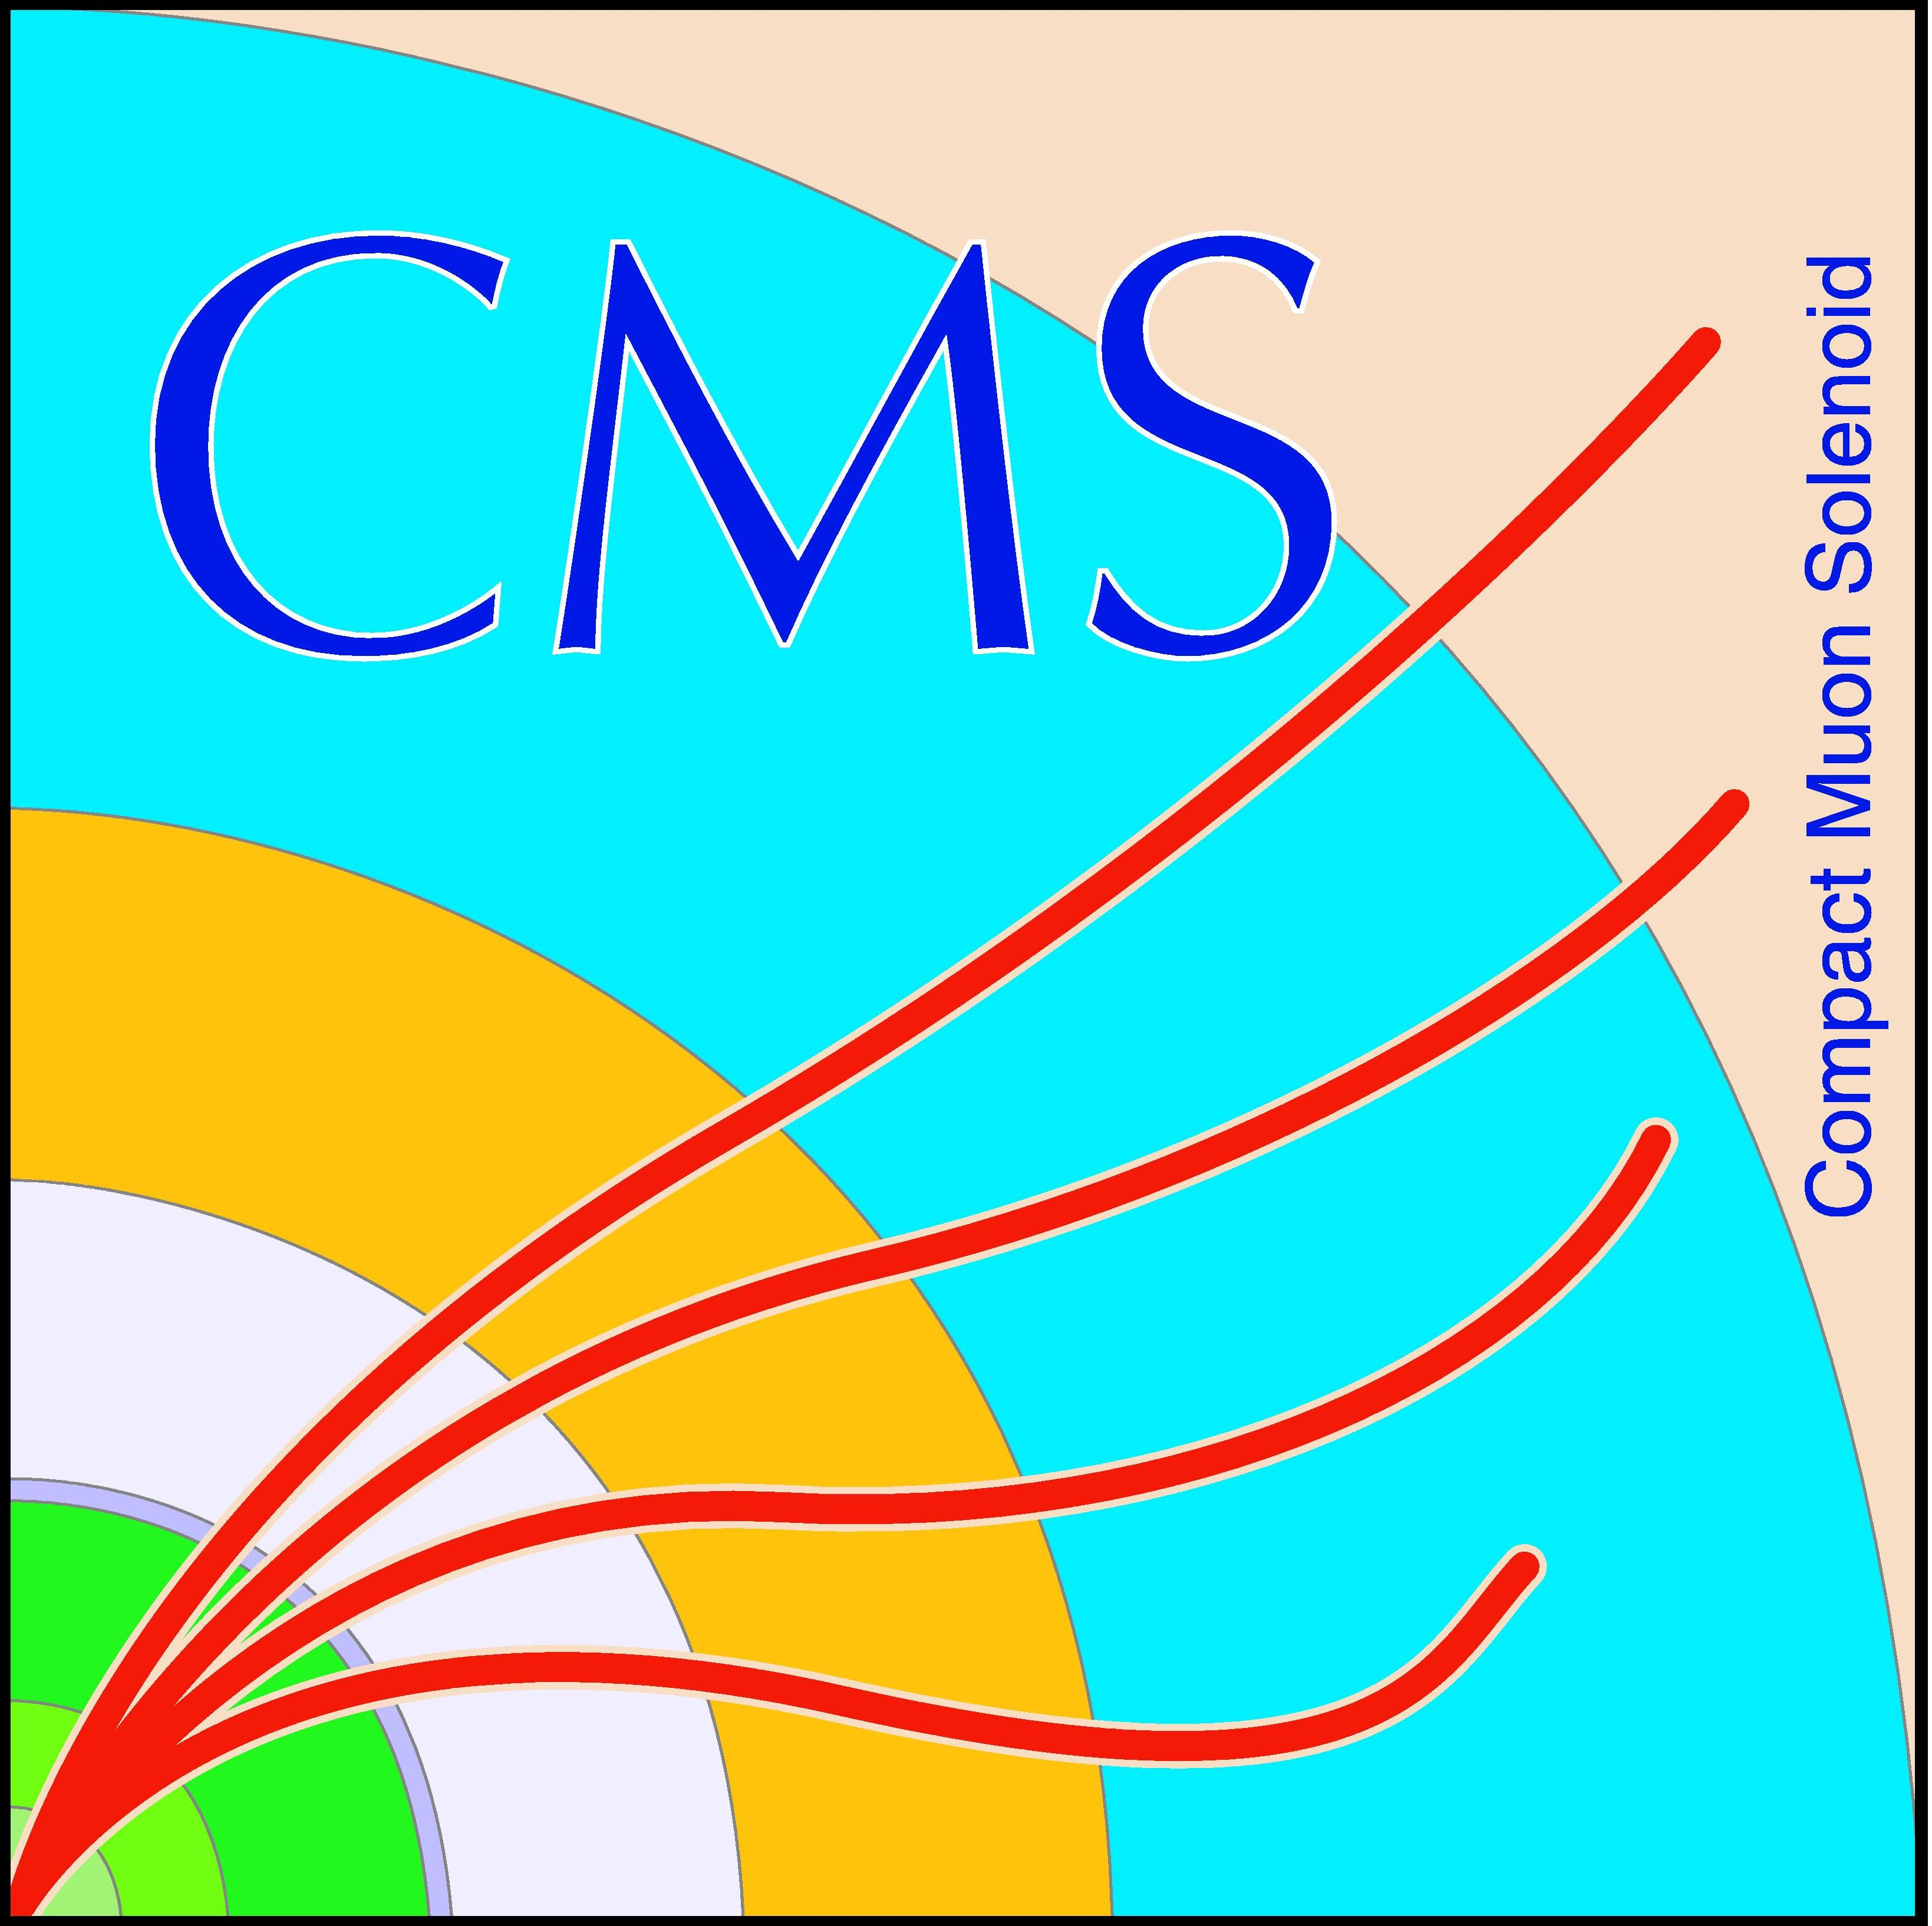
\includegraphics[height=1.5cm]{CMSlogo.jpeg}
  \end{center}
}

% pdflatex packages
\hypersetup{bookmarks=true}
\hypersetup{unicode=false}
\hypersetup{pdftitle={Lost-Lepton}}
\hypersetup{pdfauthor={Arne-Rasmus~Dr\"ager}}


\begin{document}
% ==================================================
% --------------------------------------------------
\begin{frame}
  \titlepage
\end{frame}

\section{Classical Lost-Lepton Method}
\begin{frame}
 \frametitle{Outline}
 \begin{itemize}
  \item Classical Lost-Lepton Method: 
  \begin{itemize}
   \item Isolated track prediction upgrade
  \end{itemize}
  \item Validation of Lepton Efficiencies:
  \begin{itemize}
   \item Electron and muon Tag\&Probe: Iso/Reco validation
   \item Isoalted tracks:
   \begin{itemize}
    \item Isolated e
    \item Isolated $\mu$
    \item Isoalted $\pi$ from $\tau_{had}$
   \end{itemize}
  \end{itemize}
 \end{itemize}
\end{frame}

\begin{frame}
 \begin{block}{}
 \centering
 \Large Classical Lost-Lepton Method: Isolated track bkg reduction closure
 \end{block}
\end{frame}

\subsection{Concept}
\begin{frame}
\frametitle{Rejection of \wpj \& \ttbar events ($W\rightarrow e,\mu$)}
 \begin{center}
\begin{tikzpicture}
    \node[anchor=south west,inner sep=0] (image) at (0,0) {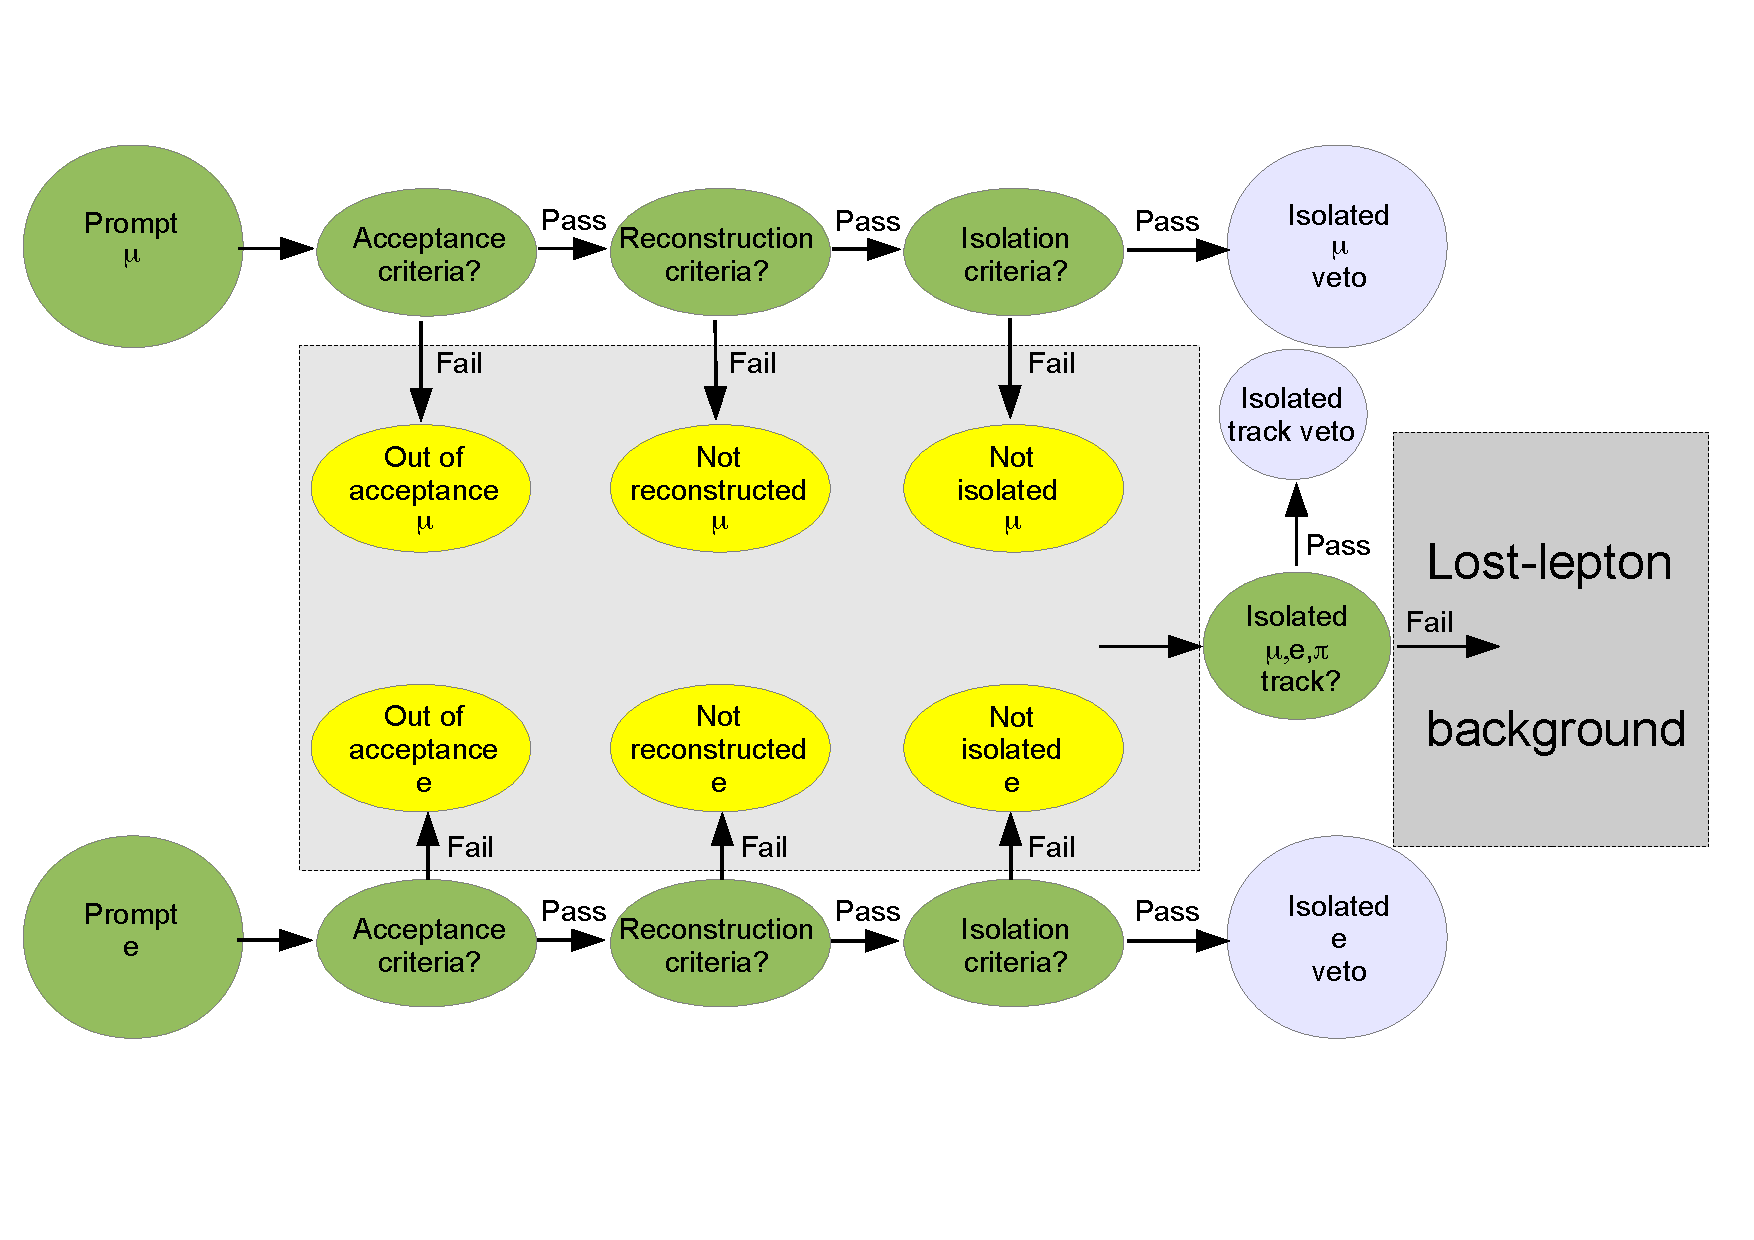
\includegraphics[width=0.75\textwidth]{figures/Sketches/LostLeptonSketch_ll_isotrack.pdf}};
    \begin{scope}[x={(image.south east)},y={(image.north west)}]
%         \draw[red,ultra thick,rounded corners] (0.62,0.65) rectangle (0.78,0.75);
%         \draw[red,ultra thick,rounded corners] (0.60,0.01) rectangle (0.75,0.99); % coordinates unten links(x,y) oben rechts(x,y)
%             \draw[blue,ultra thick,rounded corners] (0.40,0.01) rectangle (0.55,0.99); % coordinates unten links(x,y) oben rechts(x,y)
    \end{scope}
\end{tikzpicture}
 \end{center}
\end{frame}

\begin{frame}
\frametitle{Classical Lost-Lepton Prediciton of Lost Isolated $e,\mu$ events}
 \begin{center}
\begin{tikzpicture}
    \node[anchor=south west,inner sep=0] (image) at (0,0) {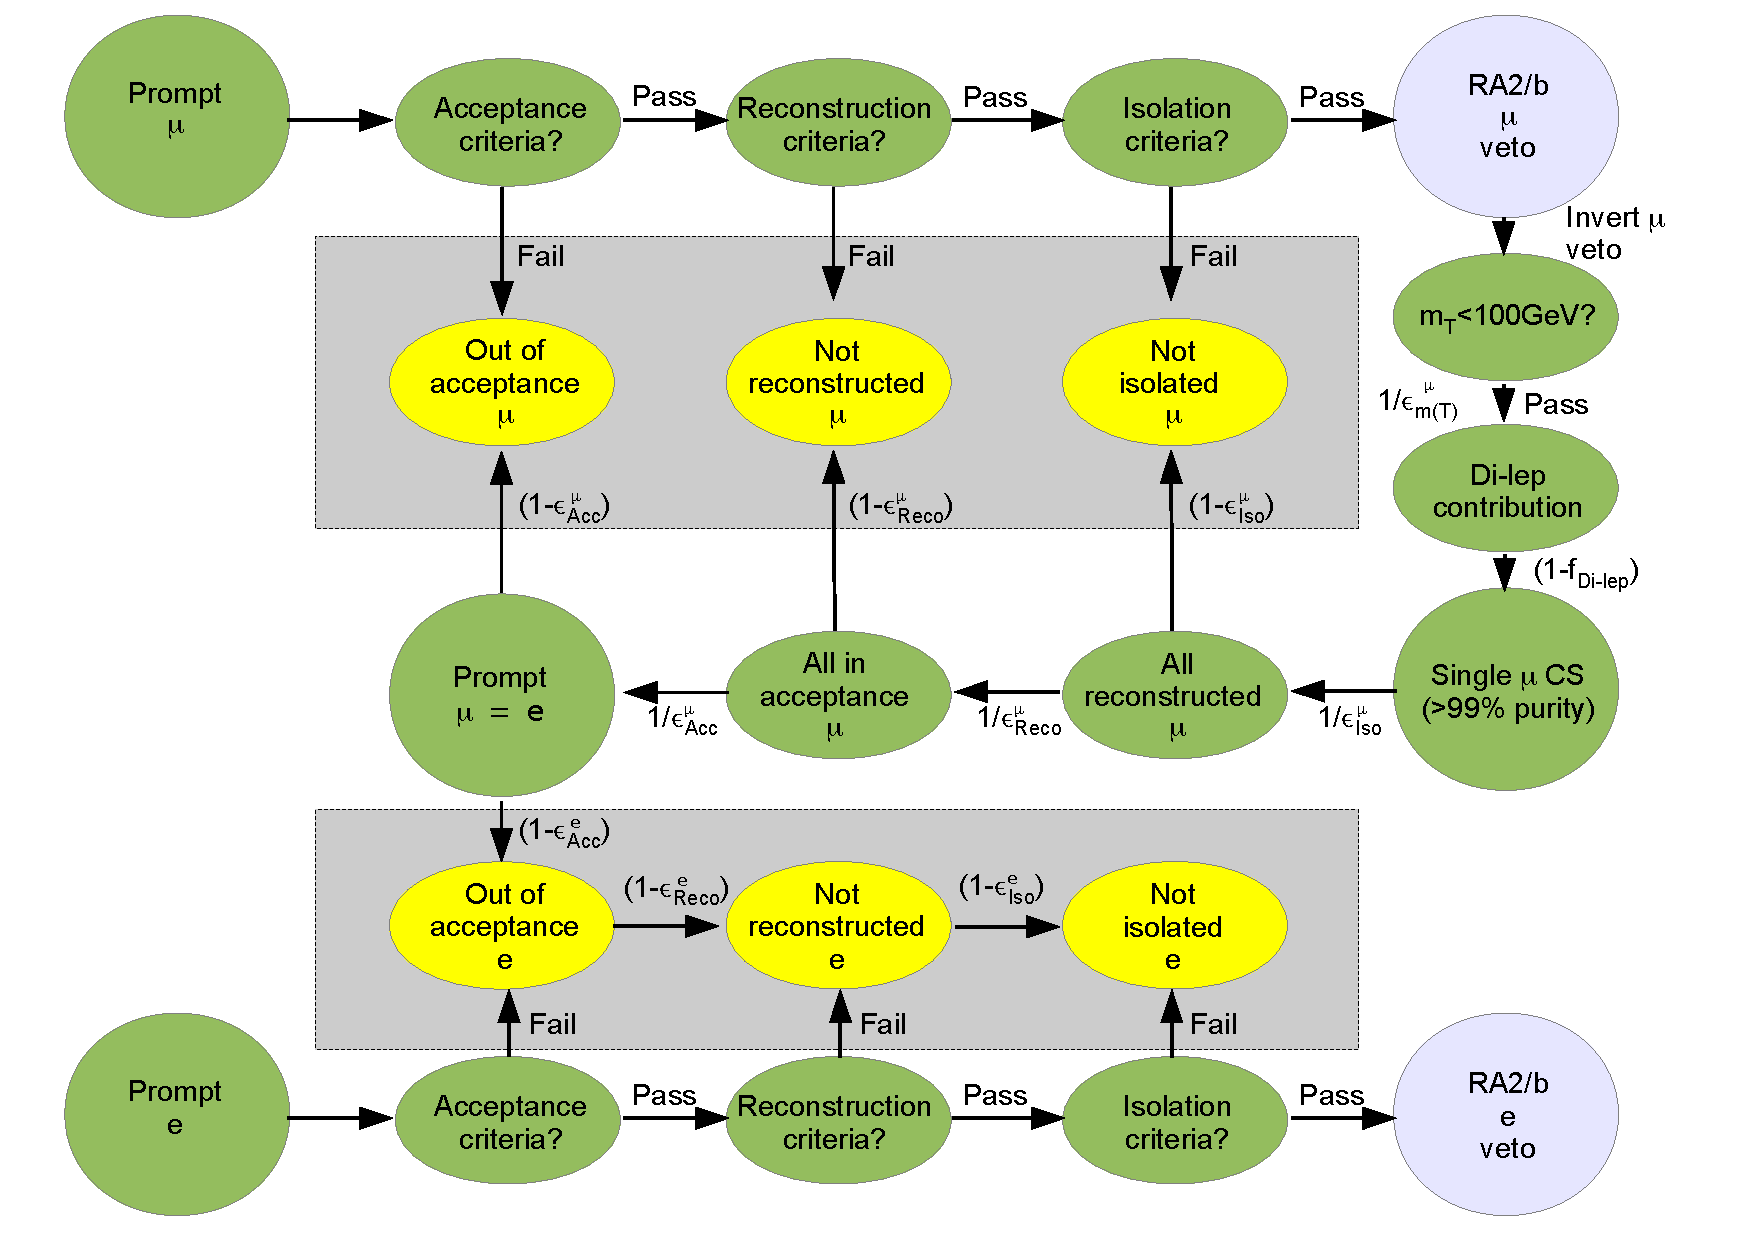
\includegraphics[width=0.75\textwidth]{figures/Sketches/LostLeptonSketch_mu_pred_full.pdf}};
    \begin{scope}[x={(image.south east)},y={(image.north west)}]
%         \draw[red,ultra thick,rounded corners] (0.62,0.65) rectangle (0.78,0.75);
%         \draw[red,ultra thick,rounded corners] (0.60,0.01) rectangle (0.75,0.99); % coordinates unten links(x,y) oben rechts(x,y)
%             \draw[blue,ultra thick,rounded corners] (0.40,0.01) rectangle (0.55,0.99); % coordinates unten links(x,y) oben rechts(x,y)
    \end{scope}
\end{tikzpicture}
 \end{center}
\end{frame}


\begin{frame}
\frametitle{Classical Lost-Lepton Procedure}
 \begin{columns}  
 \begin{column}{0.50\textwidth}
\begin{itemize}
 \item The isoalted track veto is an ADDITIONAL reduction of the \ttbar \& \wpj bkg on top of the isolated e,$\mu$ veto!
 \item Combination:
 \begin{itemize}
  \item Apply first iso e,$\mu$ veto. Do full lost-lepton prediction (disregard iso track)
  \item Correct this prediction for further reduction of bkg from isolated tracks
 \end{itemize}

\end{itemize}

   
 \end{column}
 \begin{column}{0.50\textwidth}
\begin{center}
\begin{tikzpicture}
    \node[anchor=south west,inner sep=0] (image) at (0,0) {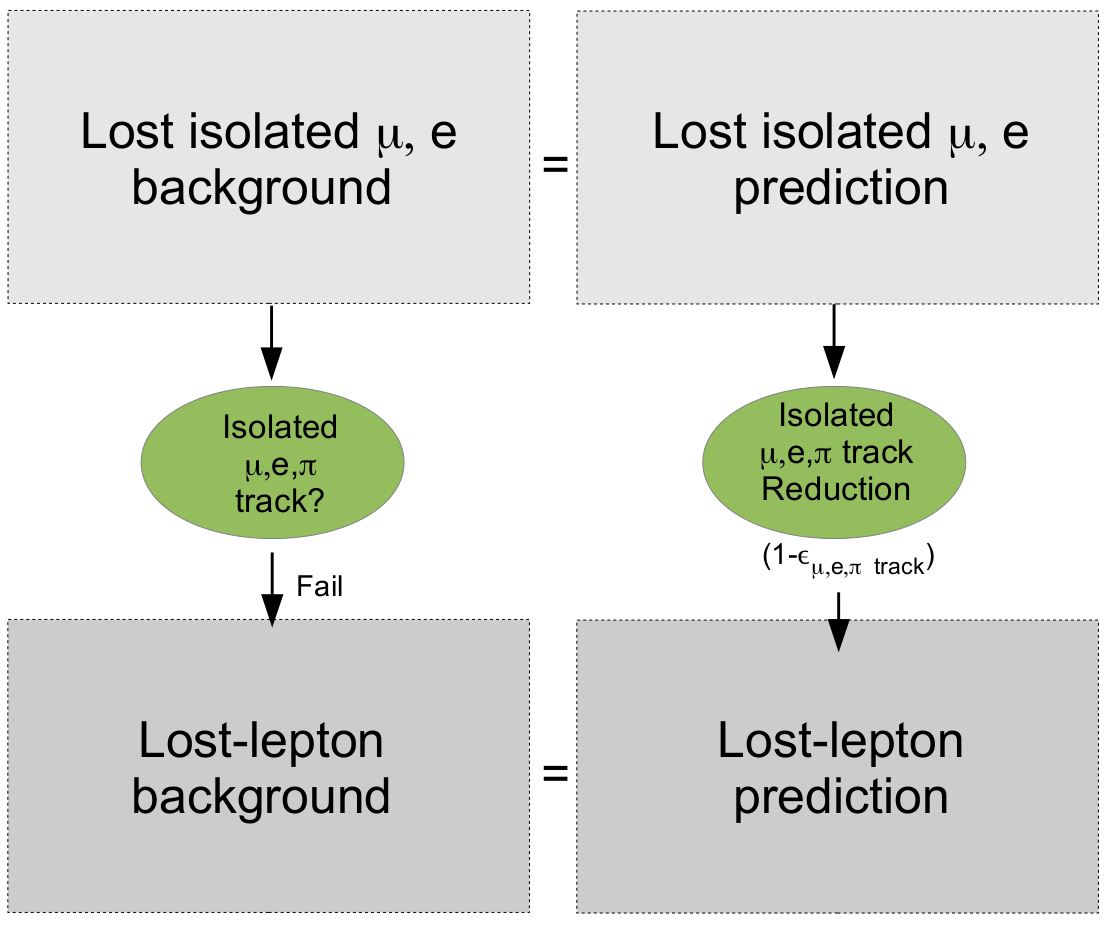
\includegraphics[width=1.\textwidth]{figures/Sketches/LostLeptonSketch_Prediction_IsoTrackReduction_small.png}};
    \begin{scope}[x={(image.south east)},y={(image.north west)}]
%         \draw[red,ultra thick,rounded corners] (0.62,0.65) rectangle (0.78,0.75);
%         \draw[red,ultra thick,rounded corners] (0.60,0.01) rectangle (0.75,0.99); % coordinates unten links(x,y) oben rechts(x,y)
%             \draw[blue,ultra thick,rounded corners] (0.40,0.01) rectangle (0.55,0.99); % coordinates unten links(x,y) oben rechts(x,y)
    \end{scope}
\end{tikzpicture}
 \end{center}
 \end{column} 
 \end{columns}
 \begin{itemize}
  \item Correction of isolated track reduction is split up in: e, $\mu$ \& $\pi$ tracks
  \item Prediction lost iso. lepton - iso track eff. = Full lost-lepton prediction
 \end{itemize}

\end{frame}
\begin{frame}
 \frametitle{Closure Tests}
\begin{columns}
 \begin{column}{0.50\textwidth}
  \begin{itemize}
   \item Closure before isotrack veto
  \end{itemize}
\begin{tikzpicture}
    \node[anchor=south west,inner sep=0] (image) at (0,0) {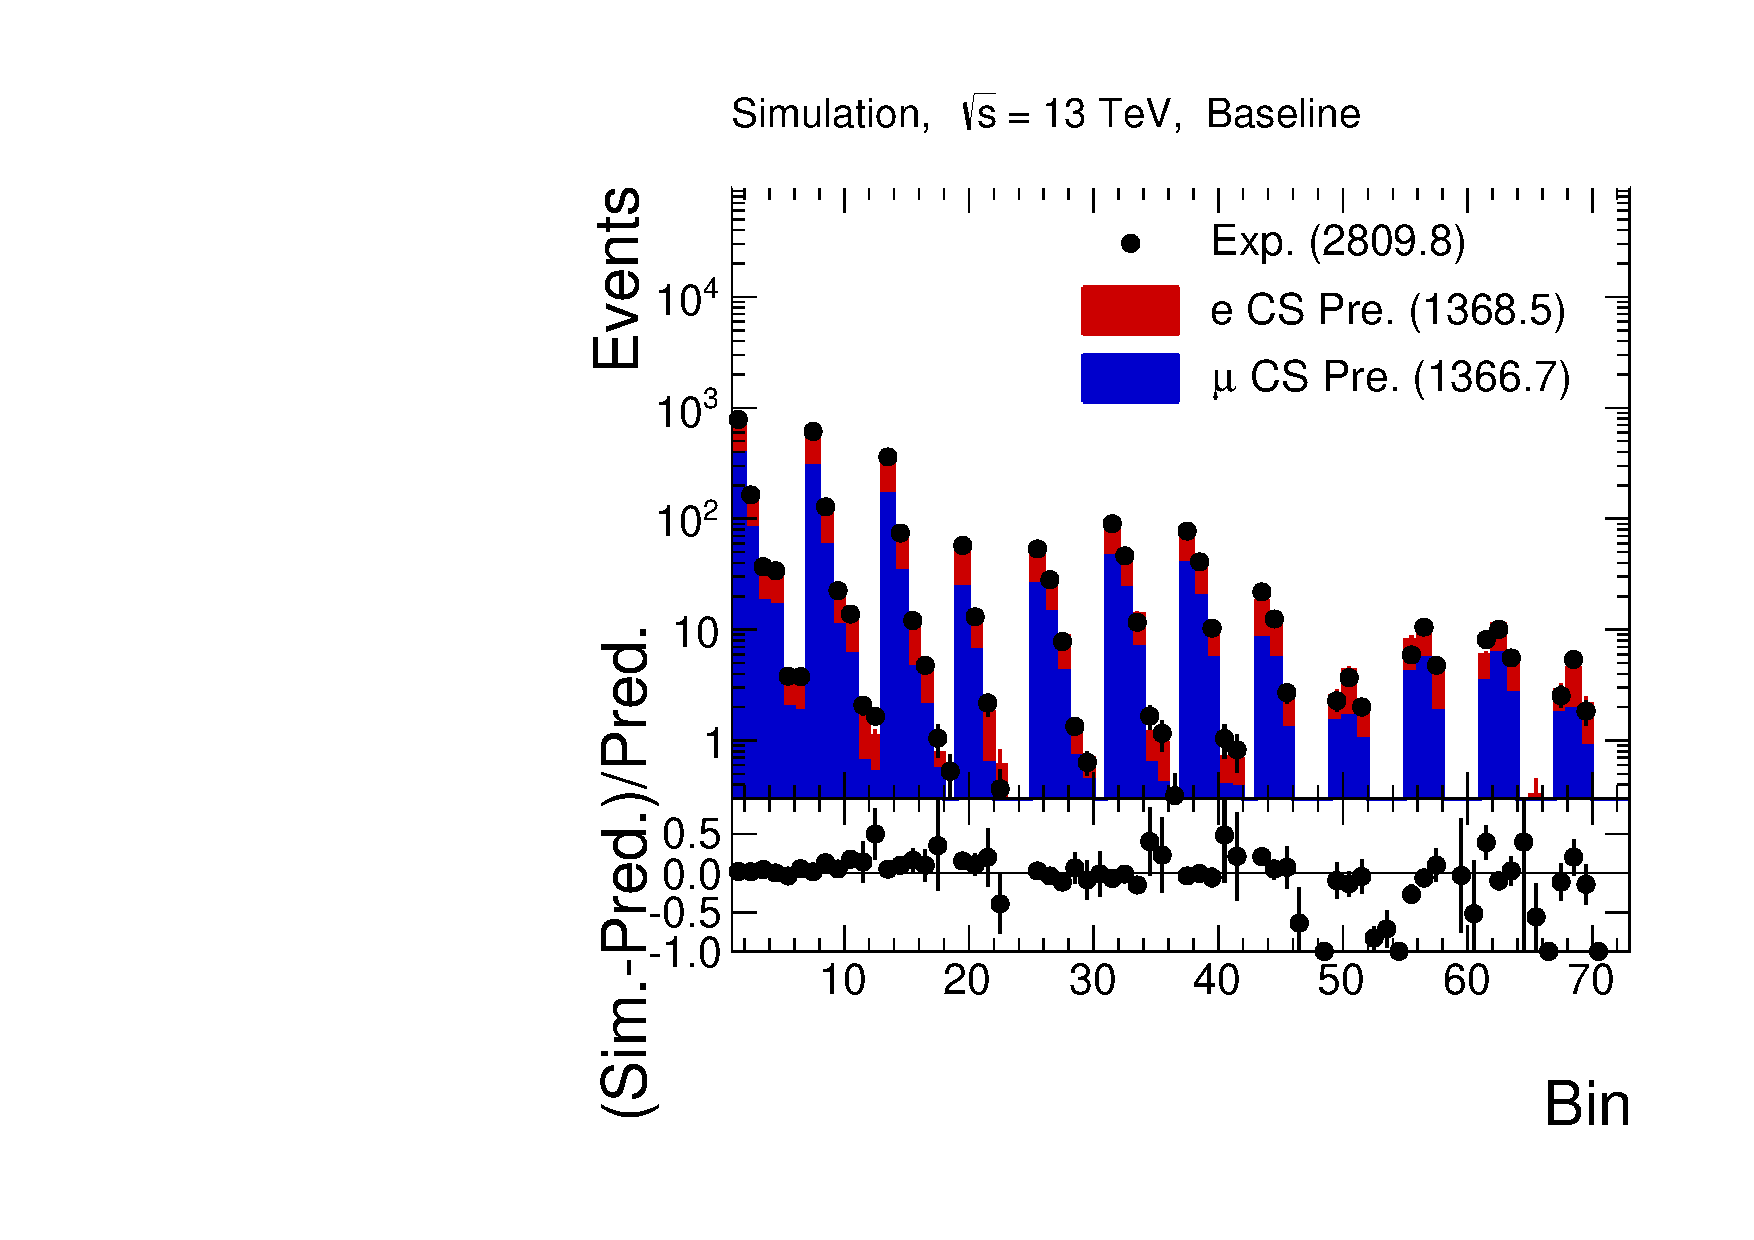
\includegraphics[width=1.\textwidth]{figures/lost-lepton_classic/Closure/Baseline/Closure__Bin__MCEx_vs_MuPrMTWDiLep+ElecPrMTWDiLep__Baseline.pdf}};
    \begin{scope}[x={(image.south east)},y={(image.north west)}]
    \end{scope}
\end{tikzpicture}


 \end{column}
 \begin{column}{0.50\textwidth}
  \begin{itemize}
   \item Correcting for iso track veto
  \end{itemize}
\begin{tikzpicture}
    \node[anchor=south west,inner sep=0] (image) at (0,0) {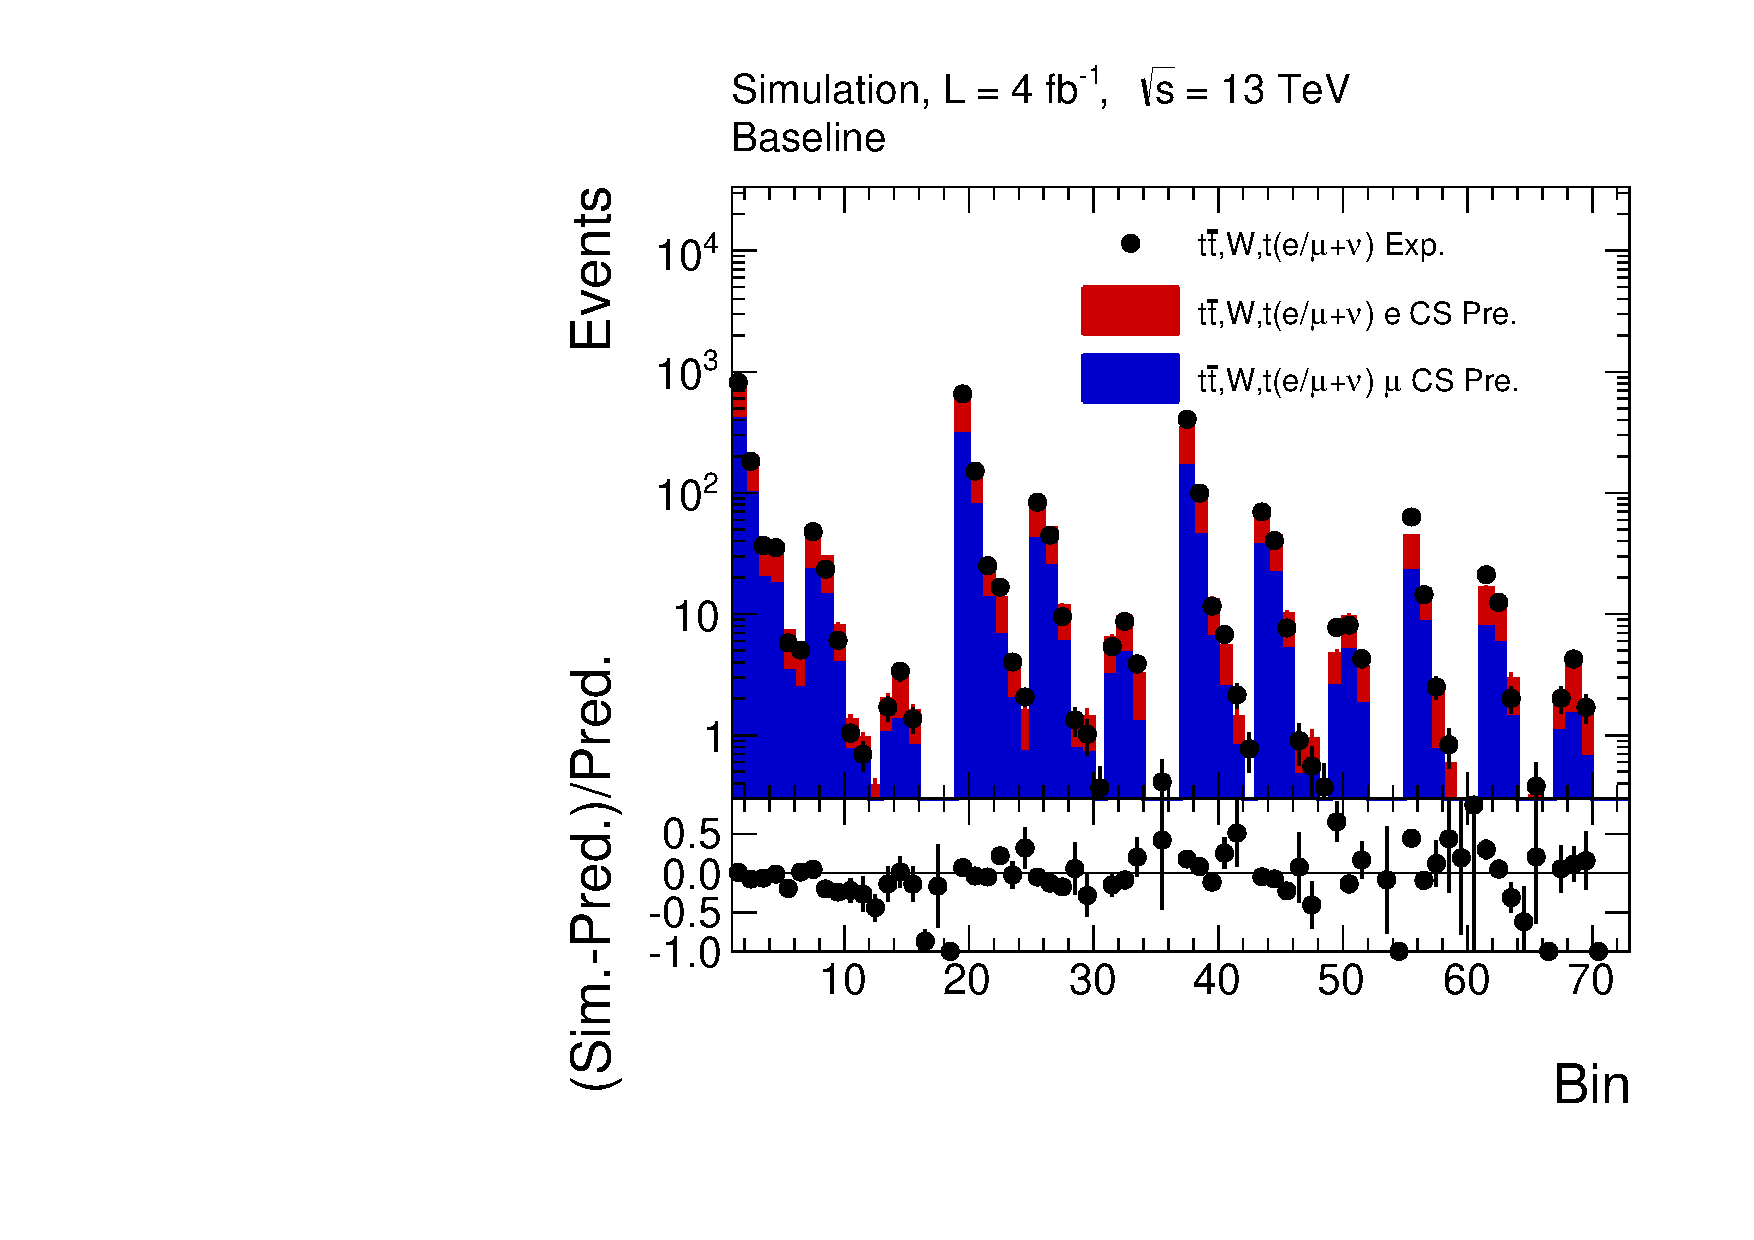
\includegraphics[width=1.\textwidth]{figures/lost-lepton_classic/Closure/Baseline/Closure__Bin__MCEx_vs_MuPrMTWDiLepIsoTrackReduced+ElecPrMTWDiLepIsoTrackReduced__Baseline.pdf}};
    \begin{scope}[x={(image.south east)},y={(image.north west)}]
    \end{scope}
\end{tikzpicture} 
 \end{column}
\end{columns}
\begin{itemize}
 \item The isolated track veto rejects about 40\% of the lost-lepton background! (w/o iso track veto: $2809.8\pm15.7$ with: $1674.1\pm12.0$)
\end{itemize}
\end{frame}

\begin{frame}
 \frametitle{Closer look at rejected events}
\begin{columns}
 \begin{column}{0.50\textwidth}
 \begin{itemize}
  \item w/o iso track veto
 \end{itemize}

\begin{tikzpicture}
    \node[anchor=south west,inner sep=0] (image) at (0,0) {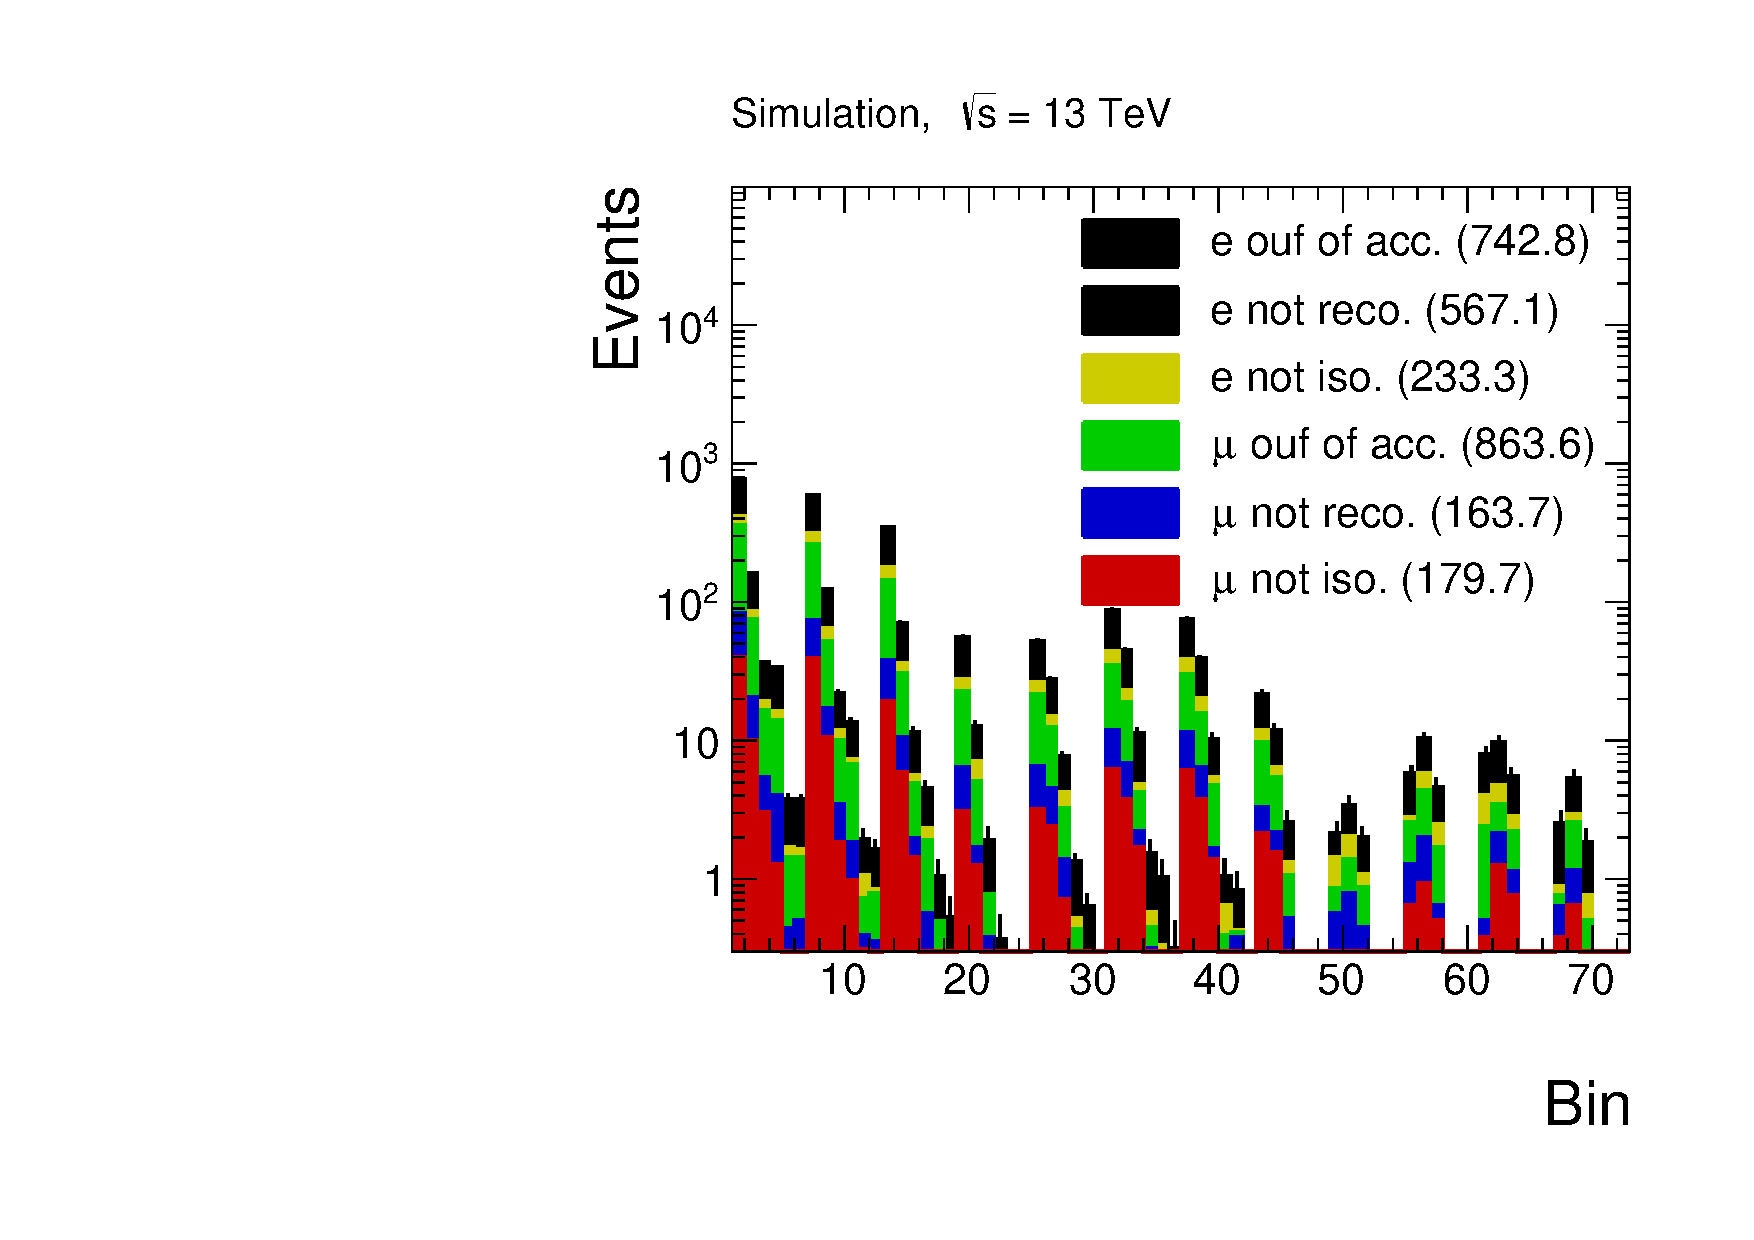
\includegraphics[width=1.\textwidth]{figures/lost-lepton_classic/Composition/Baseline_NoIsoTrack/Composition__Bin__MuIso+MuReco+MuAcc+ElecIso+ElecReco+ElecAcc__Baseline_NoIsoTrack.pdf}};
    \begin{scope}[x={(image.south east)},y={(image.north west)}]
    \end{scope}
\end{tikzpicture}
 \end{column}
 \begin{column}{0.50\textwidth}
  \begin{itemize}
  \item With iso track veto
 \end{itemize}
\begin{tikzpicture}
    \node[anchor=south west,inner sep=0] (image) at (0,0) {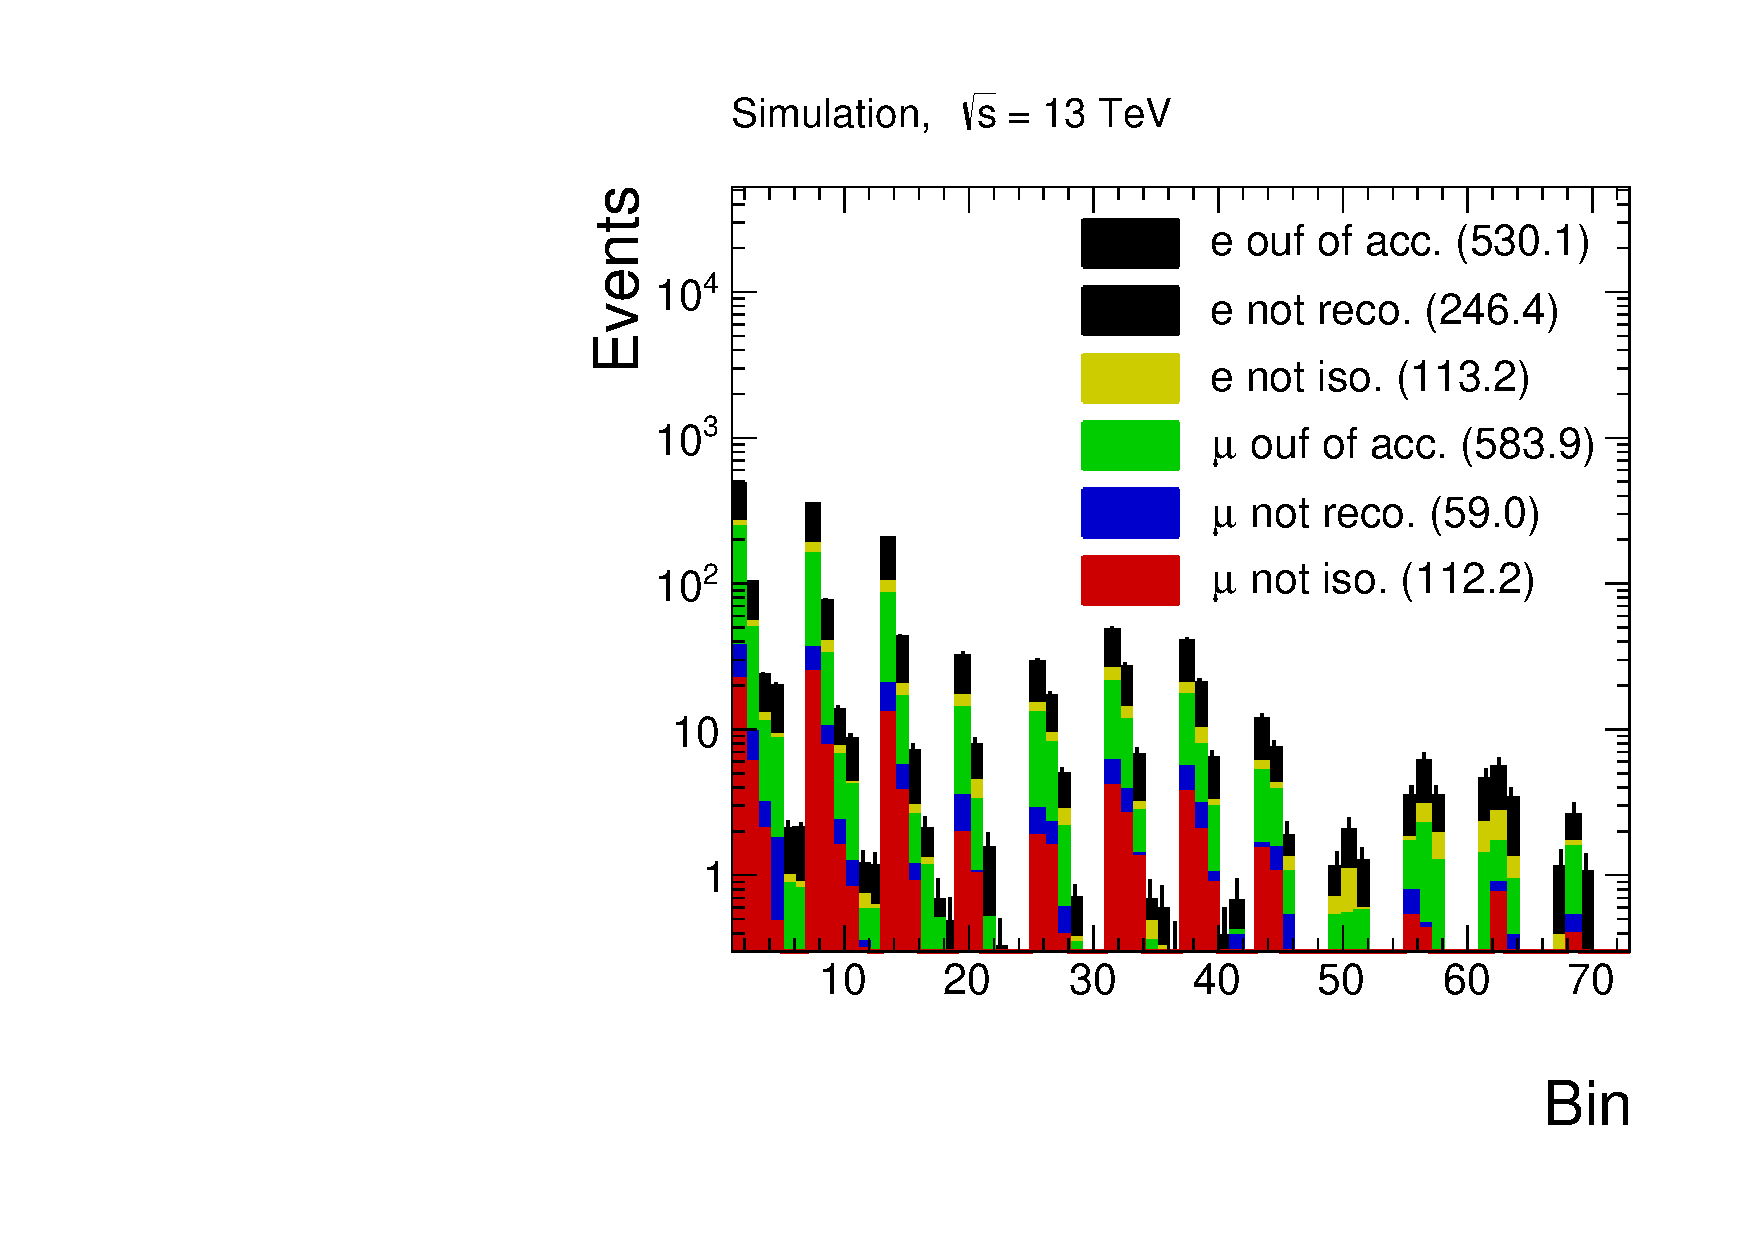
\includegraphics[width=1.\textwidth]{figures/lost-lepton_classic/Composition/Baseline/Composition__Bin__MuIso+MuReco+MuAcc+ElecIso+ElecReco+ElecAcc__Baseline.pdf}};
    \begin{scope}[x={(image.south east)},y={(image.north west)}]
    \end{scope}
\end{tikzpicture} 
 \end{column}
\end{columns}
\end{frame}


\begin{frame}
 \frametitle{Closure of Correction Fractions}
\begin{columns}
 \begin{column}{0.50\textwidth}
 \begin{center}
  \begin{tikzpicture}
    \node[anchor=south west,inner sep=0] (image) at (0,0) {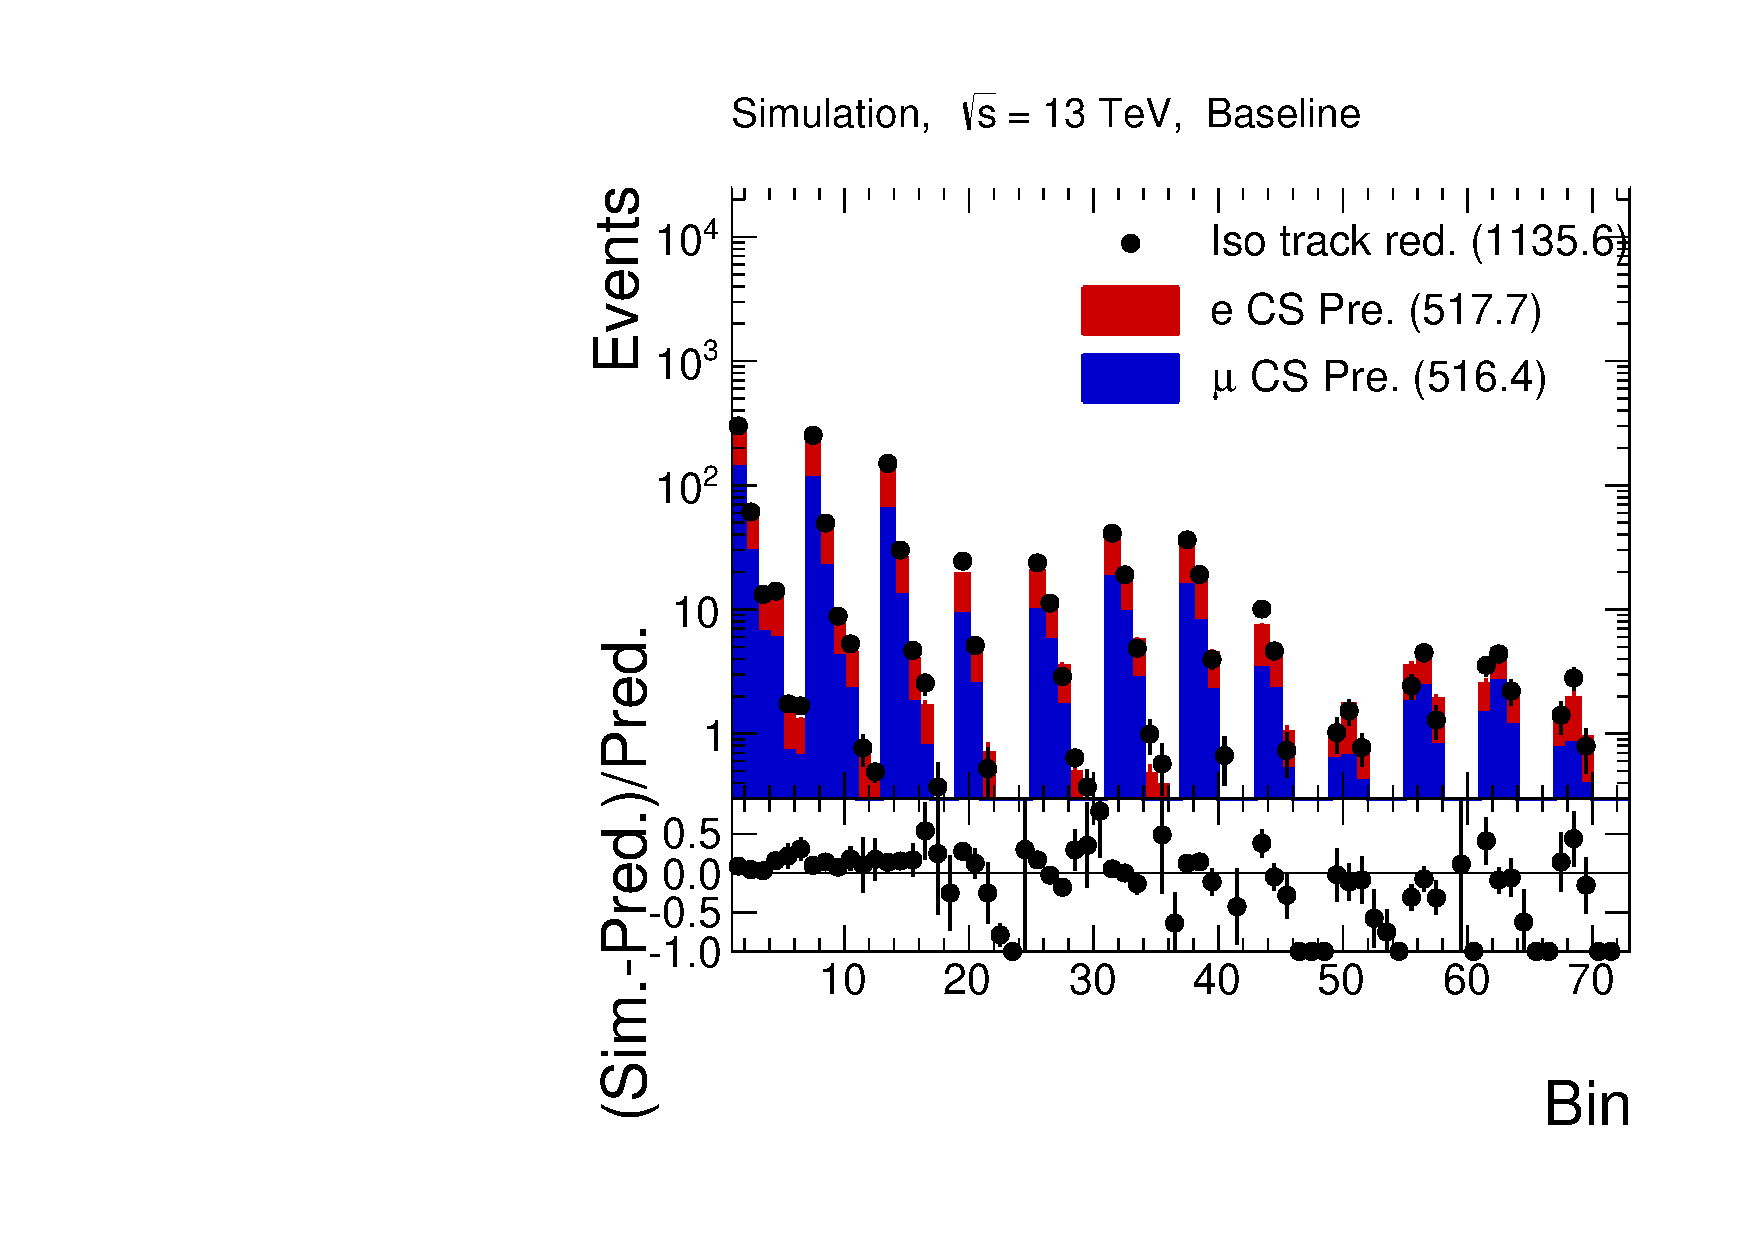
\includegraphics[width=.65\textwidth]{figures/lost-lepton_classic/Closure/Baseline/Closure__Bin__MCExIsoTrack_vs_MuPrMTWDiLepIsoTrackReduction+ElecPrMTWDiLepIsoTrackReduction__Baseline.pdf}};
    \begin{scope}[x={(image.south east)},y={(image.north west)}]
    \end{scope}
\end{tikzpicture}
\begin{tikzpicture}
    \node[anchor=south west,inner sep=0] (image) at (0,0) {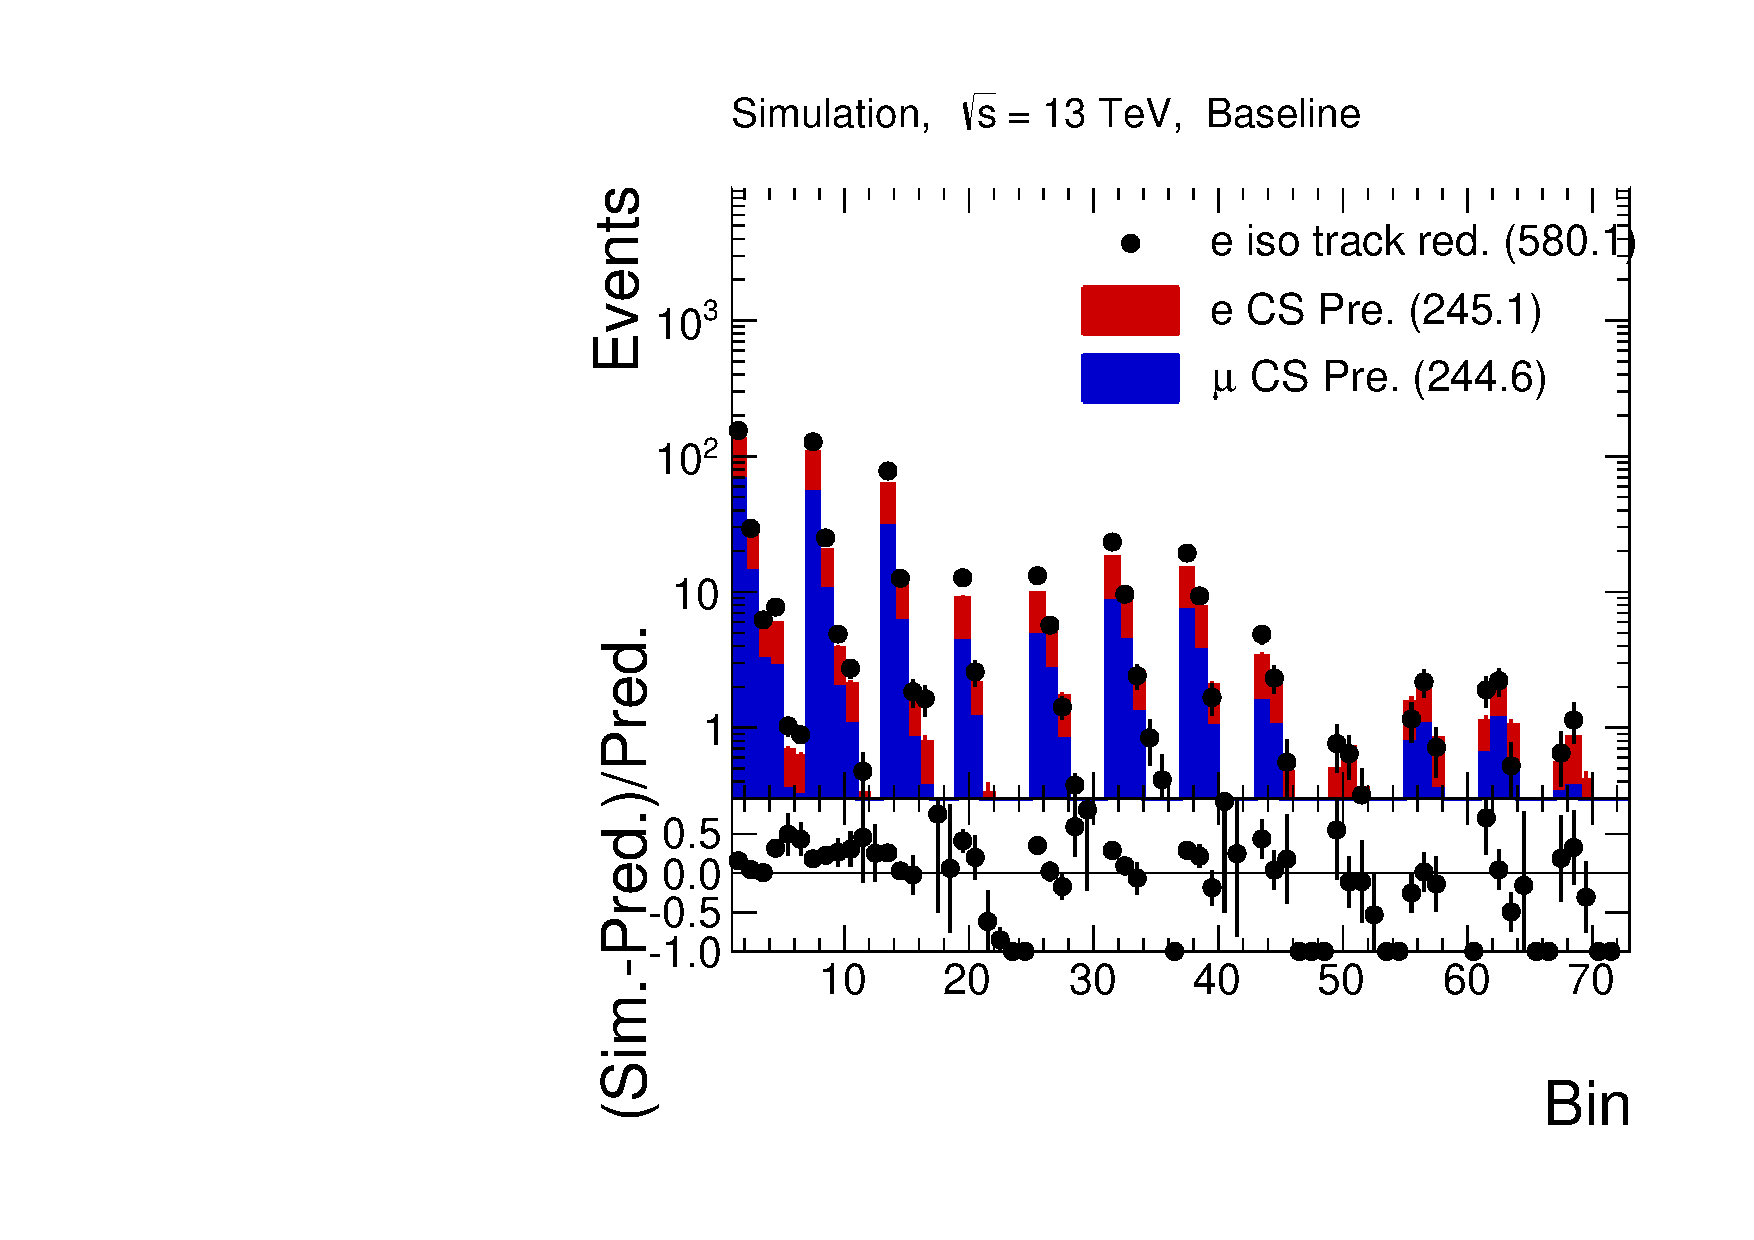
\includegraphics[width=.65\textwidth]{figures/lost-lepton_classic/Closure/Baseline/Closure__Bin__MCExElecIsoTrack_vs_MuPrMTWDiLepIsoElecTrackReduction+ElecPrMTWDiLepIsoElecTrackReduction__Baseline.pdf}};
    \begin{scope}[x={(image.south east)},y={(image.north west)}]
    \end{scope}
\end{tikzpicture} 
 \end{center}
 \end{column}
 \begin{column}{0.50\textwidth}
 \begin{center}
\begin{tikzpicture}
    \node[anchor=south west,inner sep=0] (image) at (0,0) {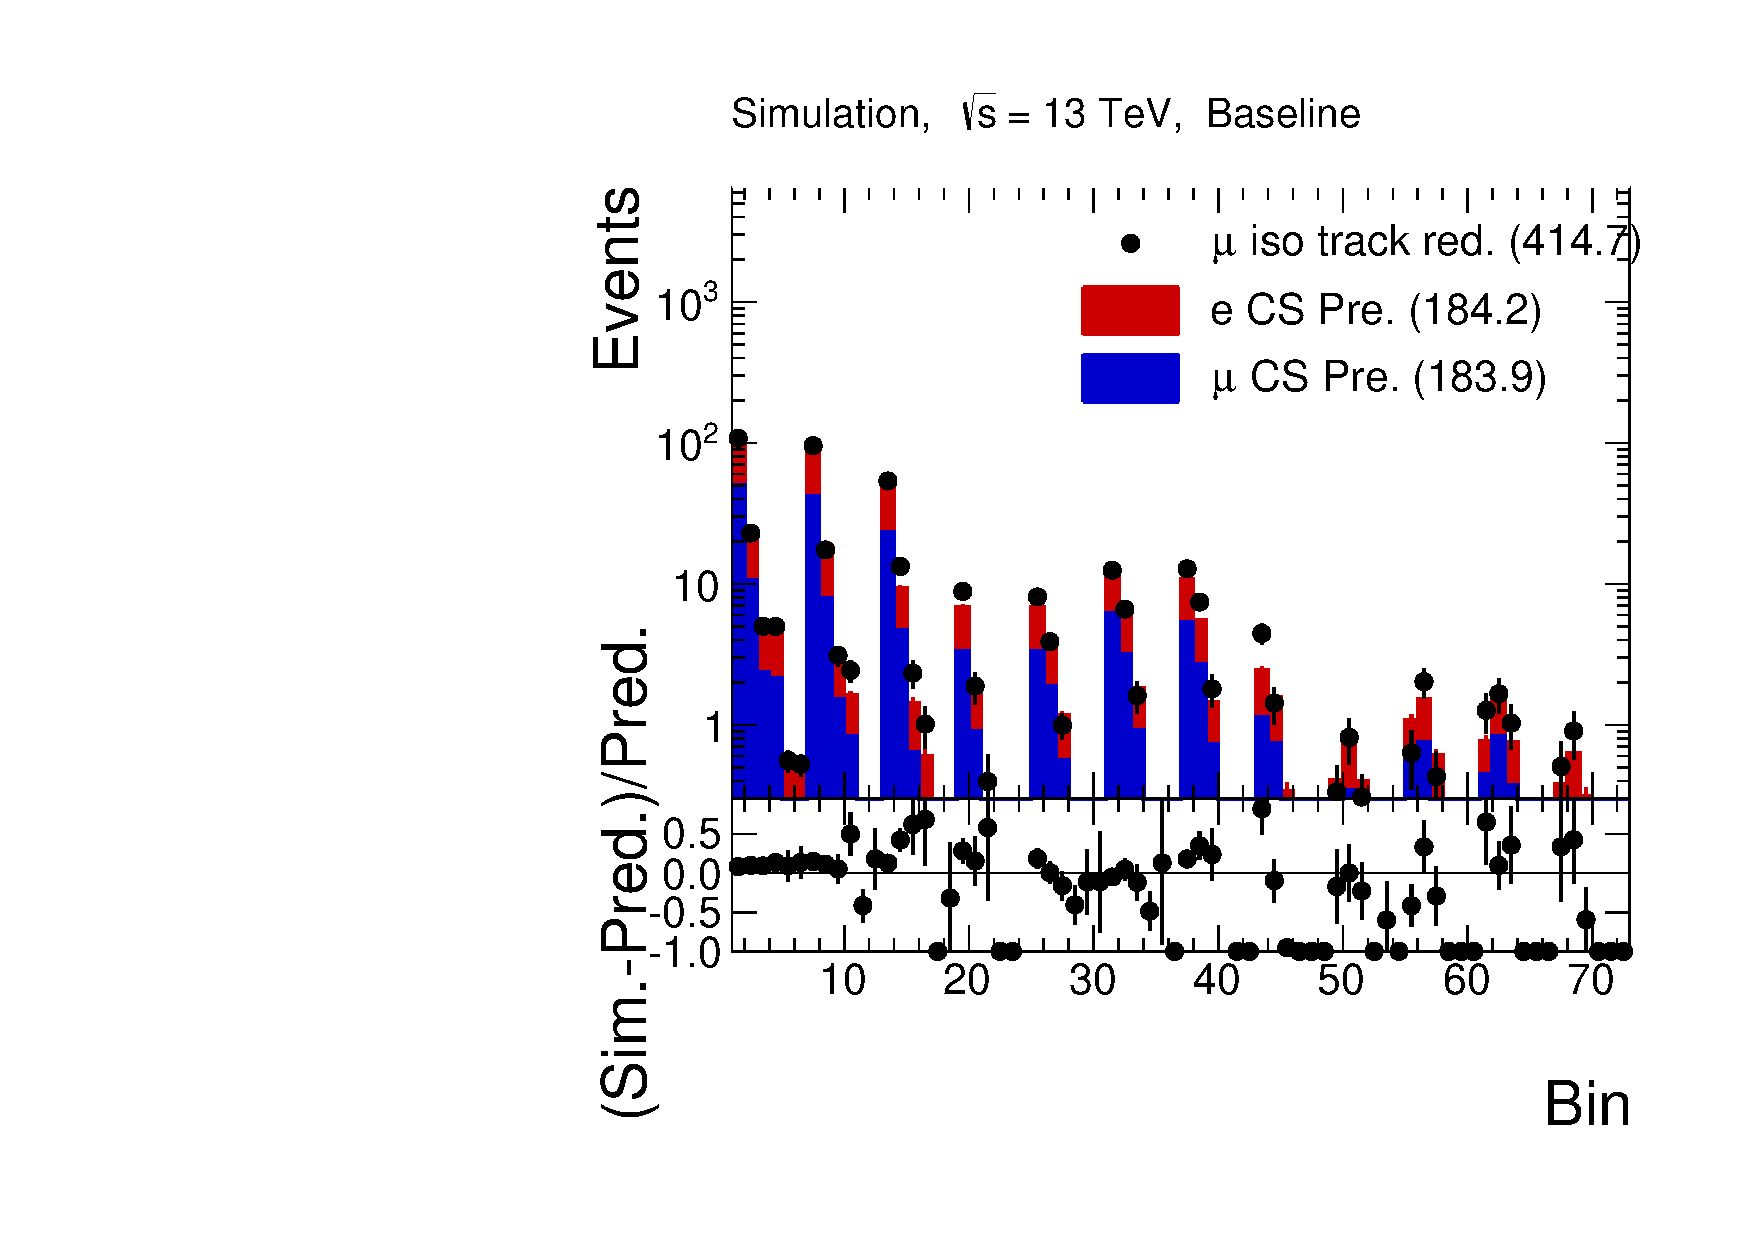
\includegraphics[width=.65\textwidth]{figures/lost-lepton_classic/Closure/Baseline/Closure__Bin__MCExMuIsoTrack_vs_MuPrMTWDiLepIsoMuTrackReduction+ElecPrMTWDiLepIsoMuTrackReduction__Baseline.pdf}};
    \begin{scope}[x={(image.south east)},y={(image.north west)}]
    \end{scope}
\end{tikzpicture} 

\begin{tikzpicture}
    \node[anchor=south west,inner sep=0] (image) at (0,0) {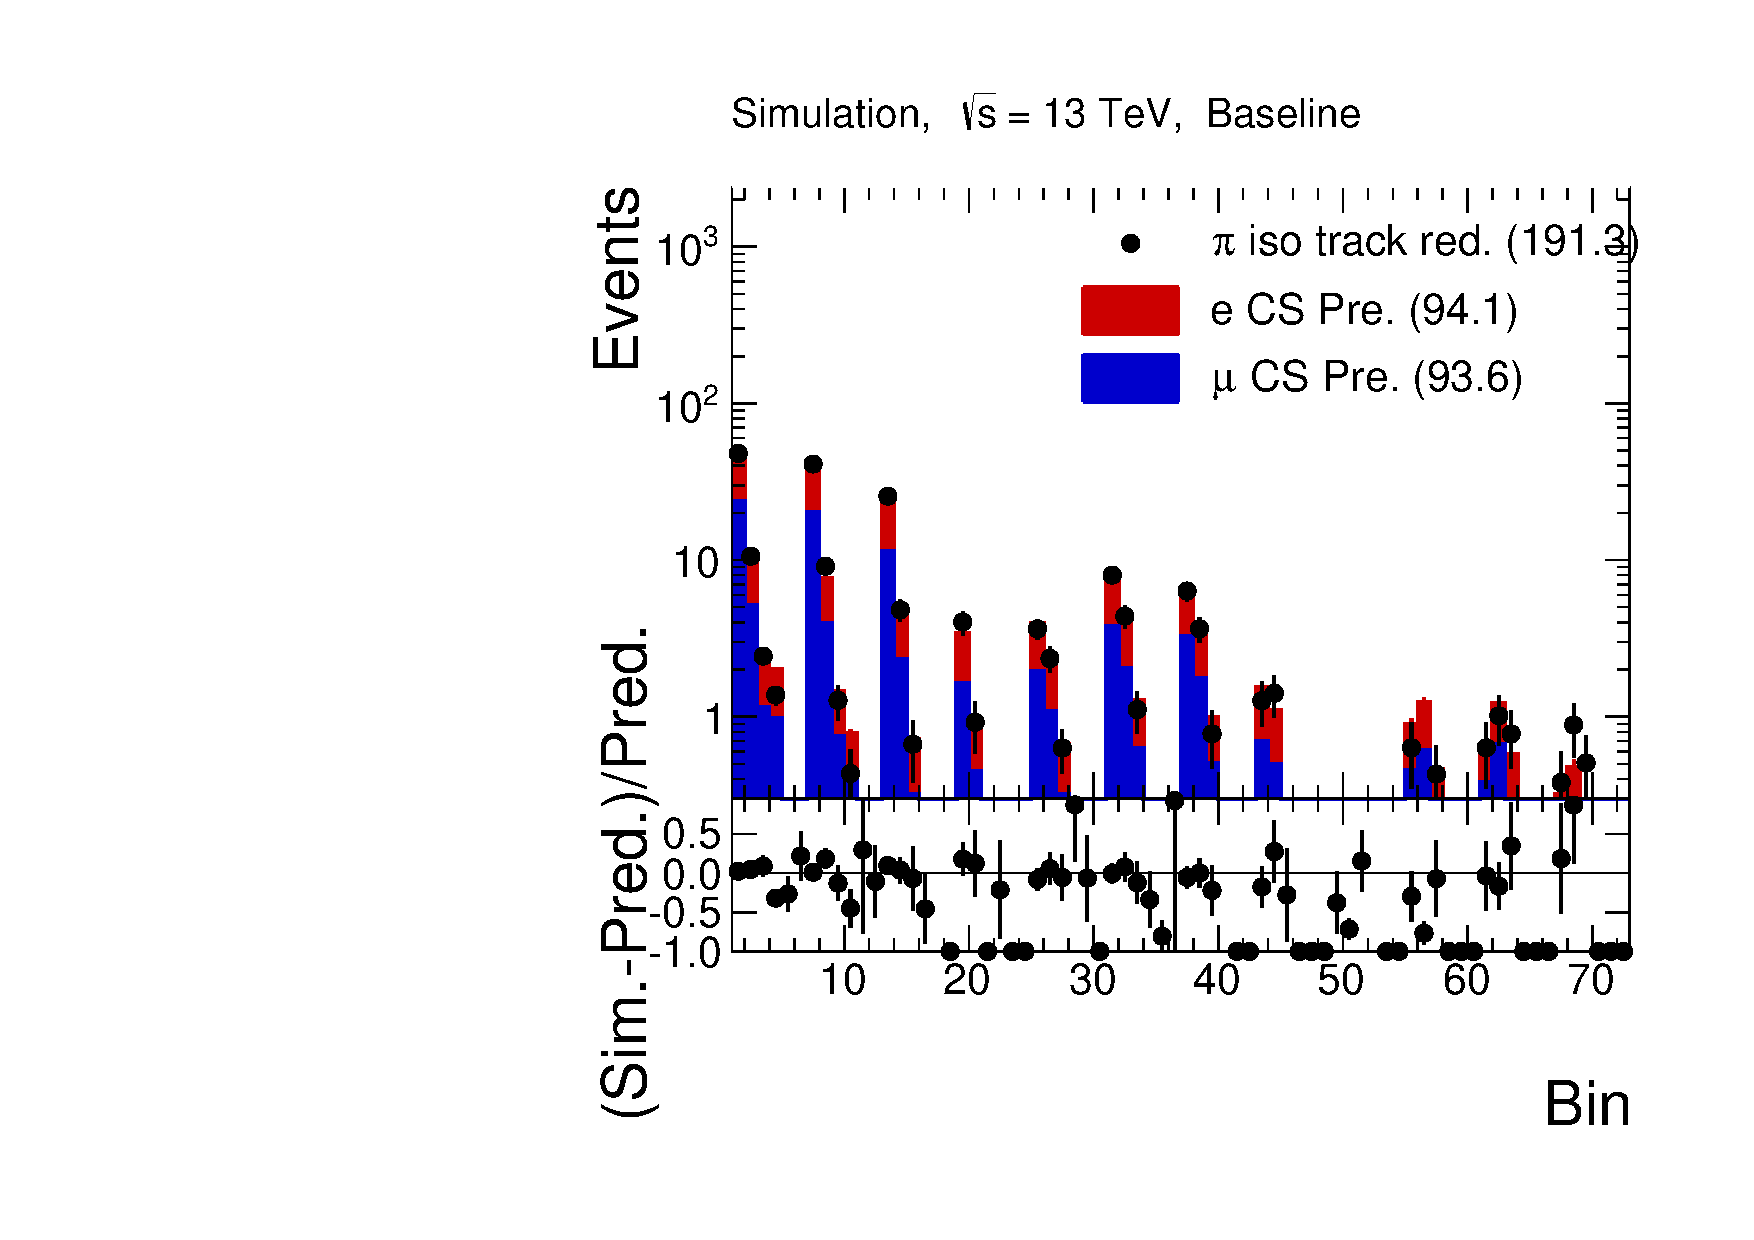
\includegraphics[width=.65\textwidth]{figures/lost-lepton_classic/Closure/Baseline/Closure__Bin__MCExPionIsoTrack_vs_MuPrMTWDiLepIsoPionTrackReduction+ElecPrMTWDiLepIsoPionTrackReduction__Baseline.pdf}};
    \begin{scope}[x={(image.south east)},y={(image.north west)}]
    \end{scope}
\end{tikzpicture} 
 \end{center}
 \end{column}
\end{columns}
\end{frame}
  


\begin{frame}
 \frametitle{Efficiencies Parametrization}

 \underline{Muon \& Electron Eff.:}
 \begin{itemize}
  \item Acc.: \HT, \MHT ,\& \NJets
  \item Reco.: \pt, Activity
  \item Iso.: \pt, Activity
  \item \mt: \NJets
  \item Di. lep. CS contribution: \NJets
  \item Di. lep. eff.: \NJets
  \item Iso. $e$ track red.: \MHT, \NJets
  \item Iso. $\mu$ track red.: \MHT, \NJets
  \item Iso. $\pi$ track red.: \MHT, \NJets
 \end{itemize} 
\end{frame}


\begin{frame}
 \begin{block}{}
 \centering
 \Large Tack\&Probe:\\Iso, Reco/ID $e,\mu$ Studies
 \end{block}
\end{frame}

\begin{frame}
\frametitle{Isolateion \& Reconstruction/ID Efficiency Studies}
 \begin{center}
\begin{tikzpicture}
    \node[anchor=south west,inner sep=0] (image) at (0,0) {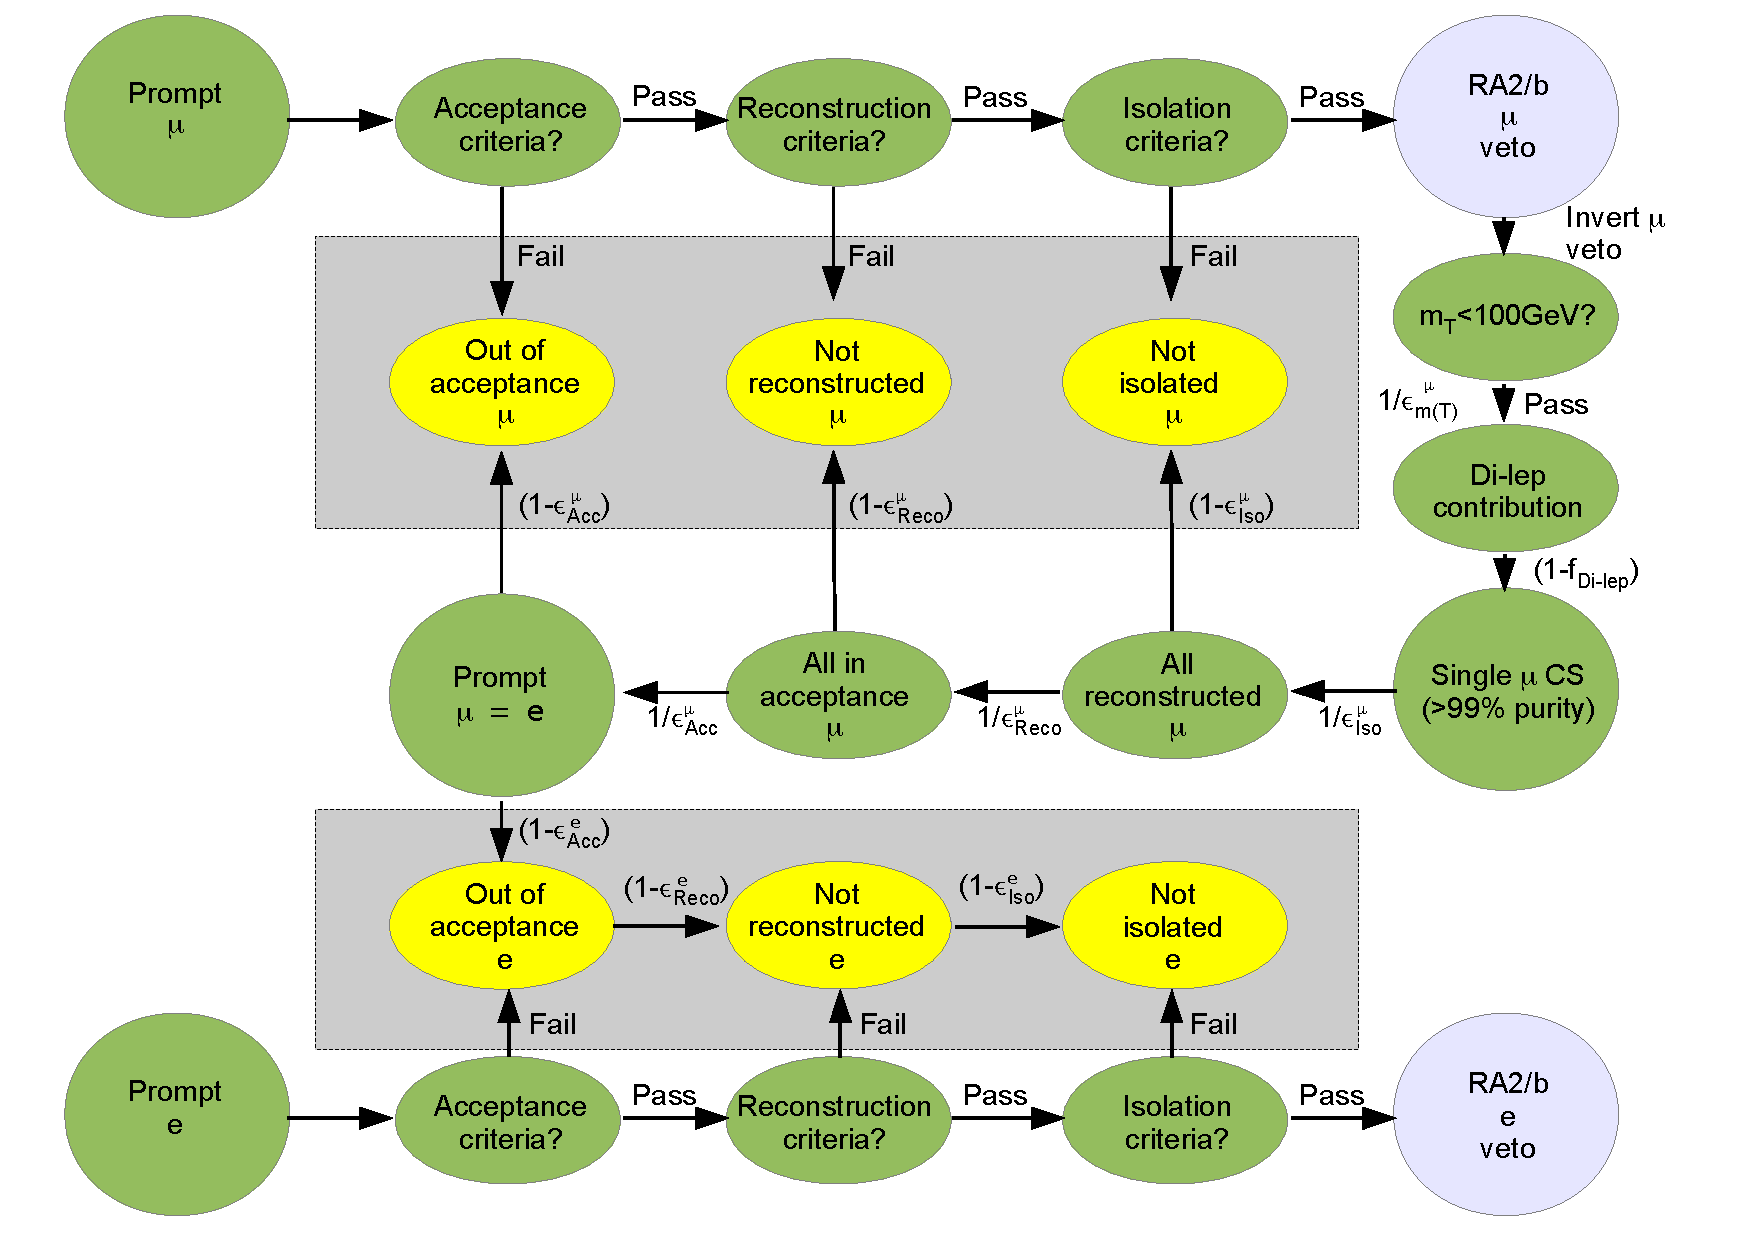
\includegraphics[width=0.75\textwidth]{figures/Sketches/LostLeptonSketch_mu_pred_full.pdf}};
    \begin{scope}[x={(image.south east)},y={(image.north west)}]
%         \draw[red,ultra thick,rounded corners] (0.62,0.65) rectangle (0.78,0.75);
        \draw[red,ultra thick,rounded corners] (0.60,0.01) rectangle (0.75,0.99); % cordinates unten links(x,y) oben rechts(x,y)
            \draw[blue,ultra thick,rounded corners] (0.40,0.01) rectangle (0.55,0.99); % cordinates unten links(x,y) oben rechts(x,y)
    \end{scope}
\end{tikzpicture}
 \end{center}
\end{frame}

\begin{frame}
 \frametitle{Tag\&Probe Reminder}
 \begin{itemize}
  \item Very established method to study (lepton) efficiencies in Data
  \item Need it to obtain/validate our MC efficiencies in Data
  \end{itemize}
  
  \begin{columns}
 \begin{column}{0.50\textwidth}
 
   \begin{itemize}

  \item Tag\&Probe Concept:
  \begin{itemize}
   \item Select a well understood topology e.g. \Zll evnts
   \item Achieve good ratio of \Zll to other events!
   \item Select Tag object: E.g. well isolated $\mu,e$
   \item Select to be tested object (Probe): Lose defined $\mu,e$. Apply to be tested criteria e.g. isolation to probe object
   \item Compute for passing(p)/failing(f) events invariant mass of di-lepton system (Z mass). 
  \end{itemize}

 \end{itemize}
 \end{column}
  \begin{column}{0.50\textwidth}
\begin{tikzpicture}
    \node[anchor=south west,inner sep=0] (image) at (0,0) {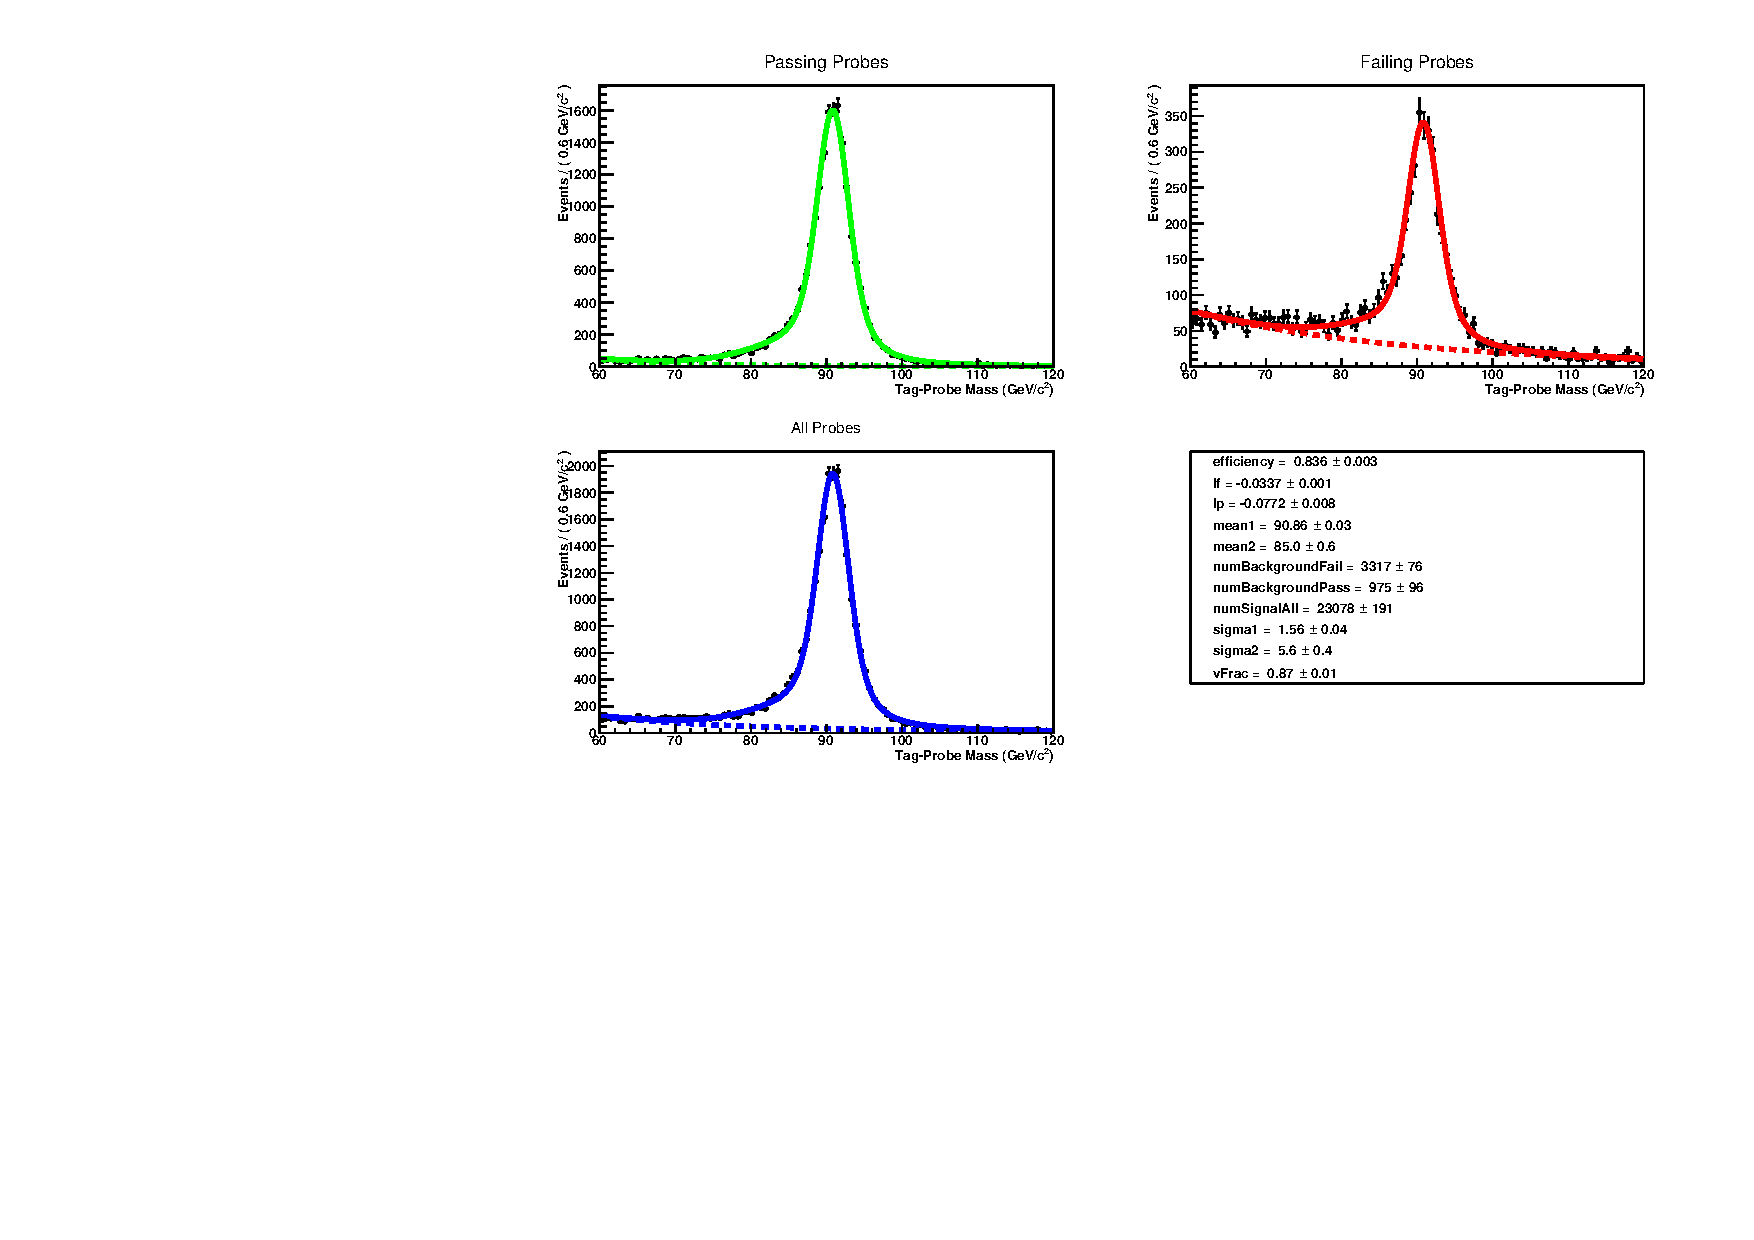
\includegraphics[width=1.\textwidth]{figures/efficiencies/tagandprobe/MuIso_Example_TagAndProbe_Fit.pdf}};
    \begin{scope}[x={(image.south east)},y={(image.north west)}]
%         \draw[red,ultra thick,rounded corners] (0.62,0.65) rectangle (0.78,0.75);
    \end{scope}
\end{tikzpicture}  
\begin{itemize}
 \item Fit passing/failing Z mass distribution: Function: Z resonance \& background shape
 \item $Eff. = p / (p + f)$  
\end{itemize}
  \end{column}
 \end{columns}
\end{frame}

\begin{frame}
 \frametitle{$\mu$ Isolation Efficiencies}
  \begin{columns}

   \begin{column}{0.33\textwidth}
     \begin{itemize}
   \item $\mu$ Iso \ttbar \& \wpj eff.
  \end{itemize}
    \begin{tikzpicture}
    \node[anchor=south west,inner sep=0] (image) at (0,0) {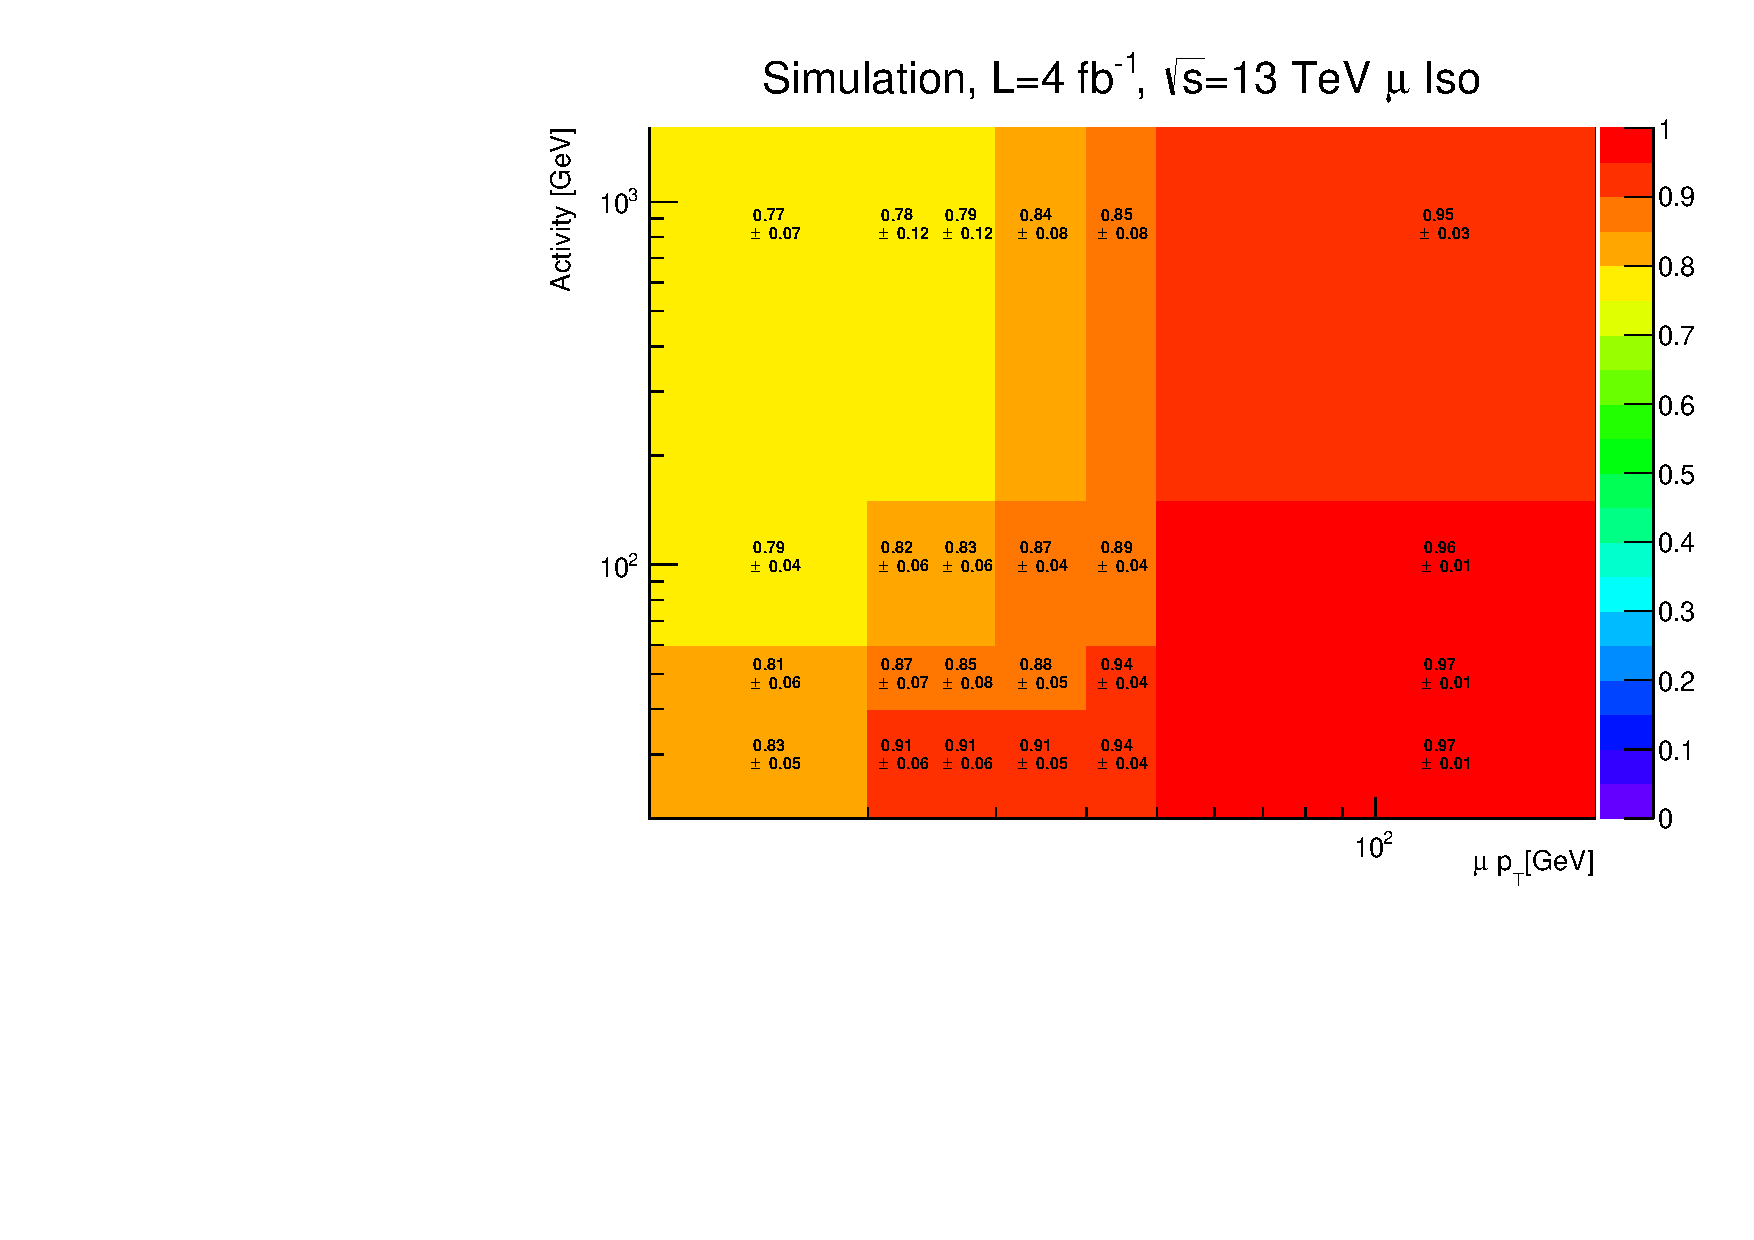
\includegraphics[width=1.\textwidth]{figures/efficiencies/ttbar-wpj/MuIsoPTActivity.pdf}};
    \begin{scope}[x={(image.south east)},y={(image.north west)}]
%         \draw[red,ultra thick,rounded corners] (0.62,0.65) rectangle (0.78,0.75);
%         \draw[red,ultra thick,rounded corners] (0.60,0.01) rectangle (0.75,0.99); % cordinates unten links(x,y) oben rechts(x,y)
    \end{scope}
   \end{tikzpicture}
   \end{column}
   \begin{column}{0.33\textwidth}
   \begin{itemize}
    \item $\mu$ Iso Tag \& Probe eff.
   \end{itemize}

    \begin{tikzpicture}
    \node[anchor=south west,inner sep=0] (image) at (0,0) {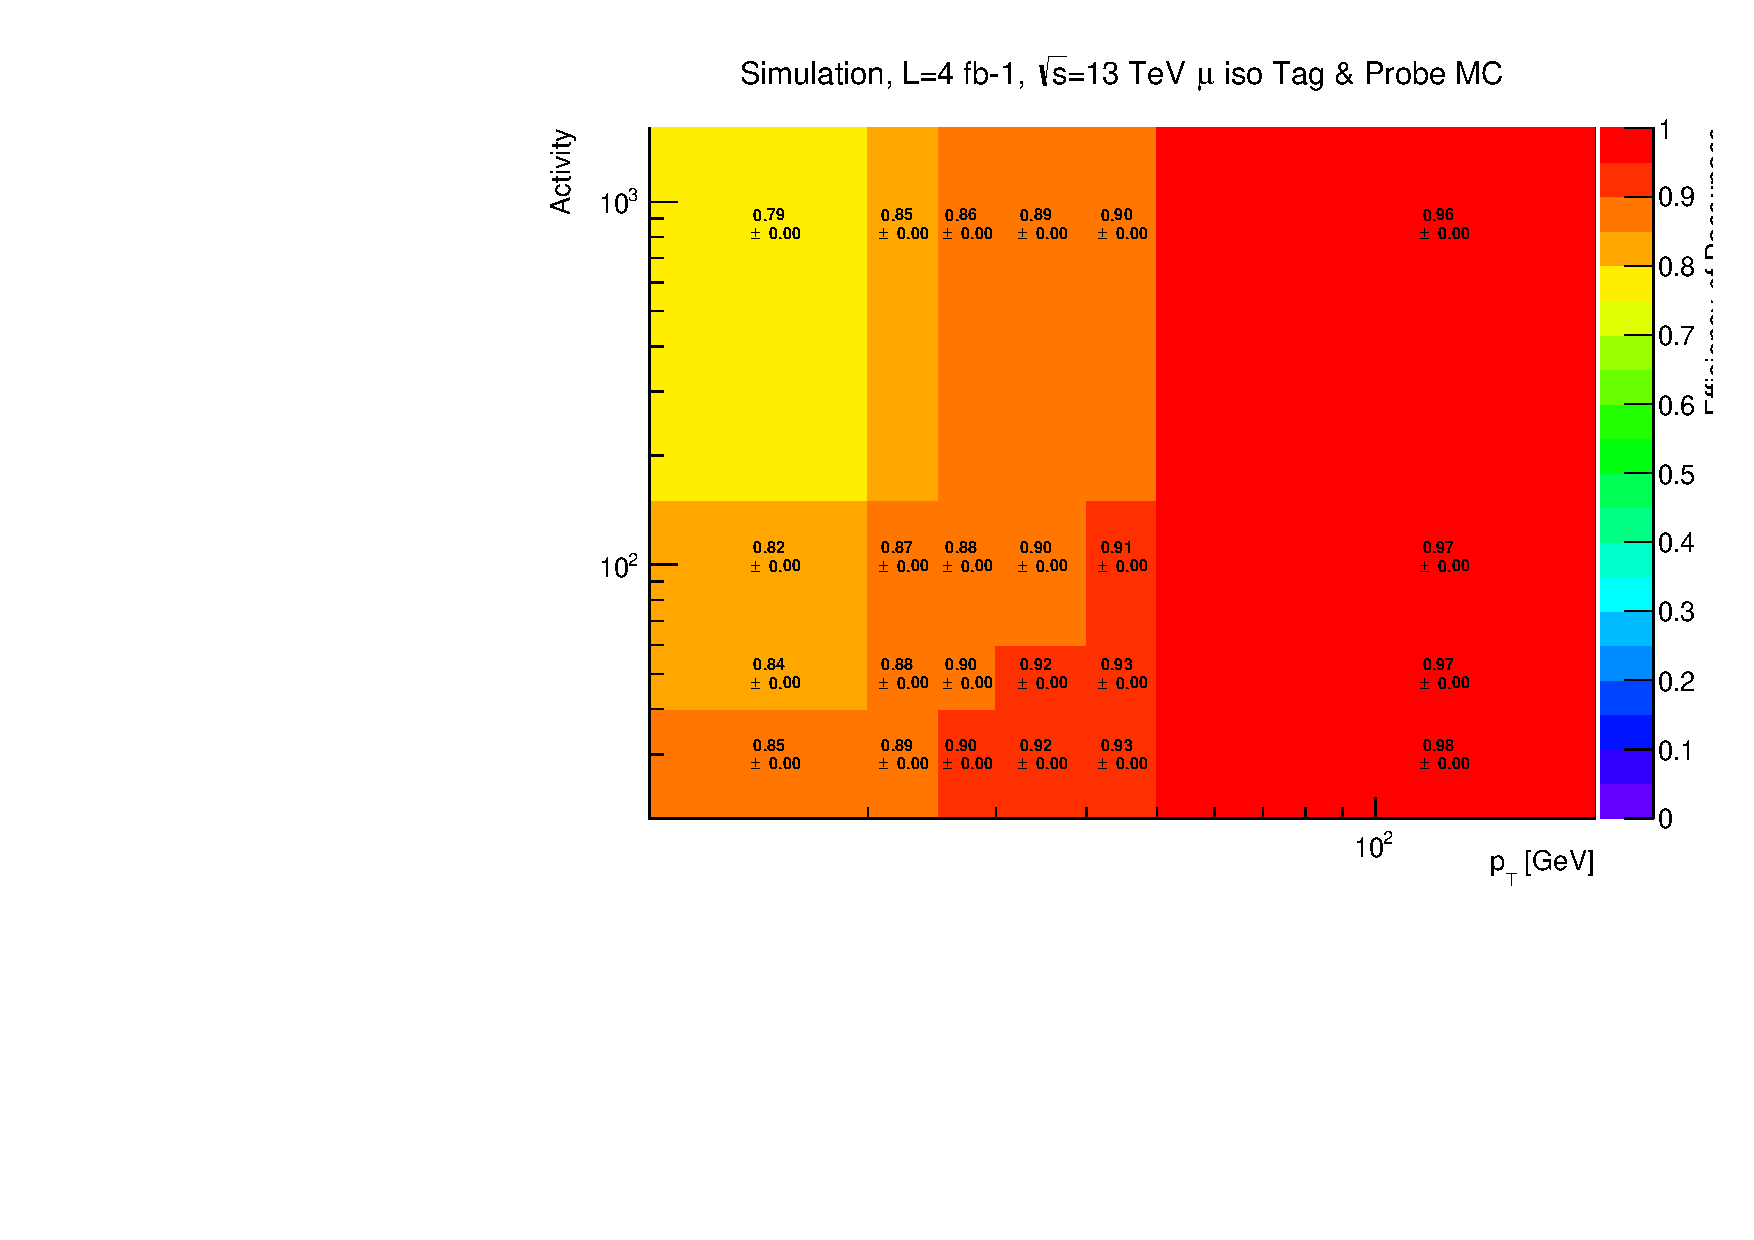
\includegraphics[width=1.\textwidth]{figures/efficiencies/tagandprobe/MuIsoTagAndProbeMC.pdf}};
    \begin{scope}[x={(image.south east)},y={(image.north west)}]
%         \draw[red,ultra thick,rounded corners] (0.62,0.65) rectangle (0.78,0.75);
%         \draw[red,ultra thick,rounded corners] (0.60,0.01) rectangle (0.75,0.99); % cordinates unten links(x,y) oben rechts(x,y)
    \end{scope}
   \end{tikzpicture}
   \end{column}
   \begin{column}{0.33\textwidth}
   \begin{itemize}
    \item Ratio: \ttbar \& \wpj / Tag \& Probe eff.
   \end{itemize}

    \begin{tikzpicture}
    \node[anchor=south west,inner sep=0] (image) at (0,0) {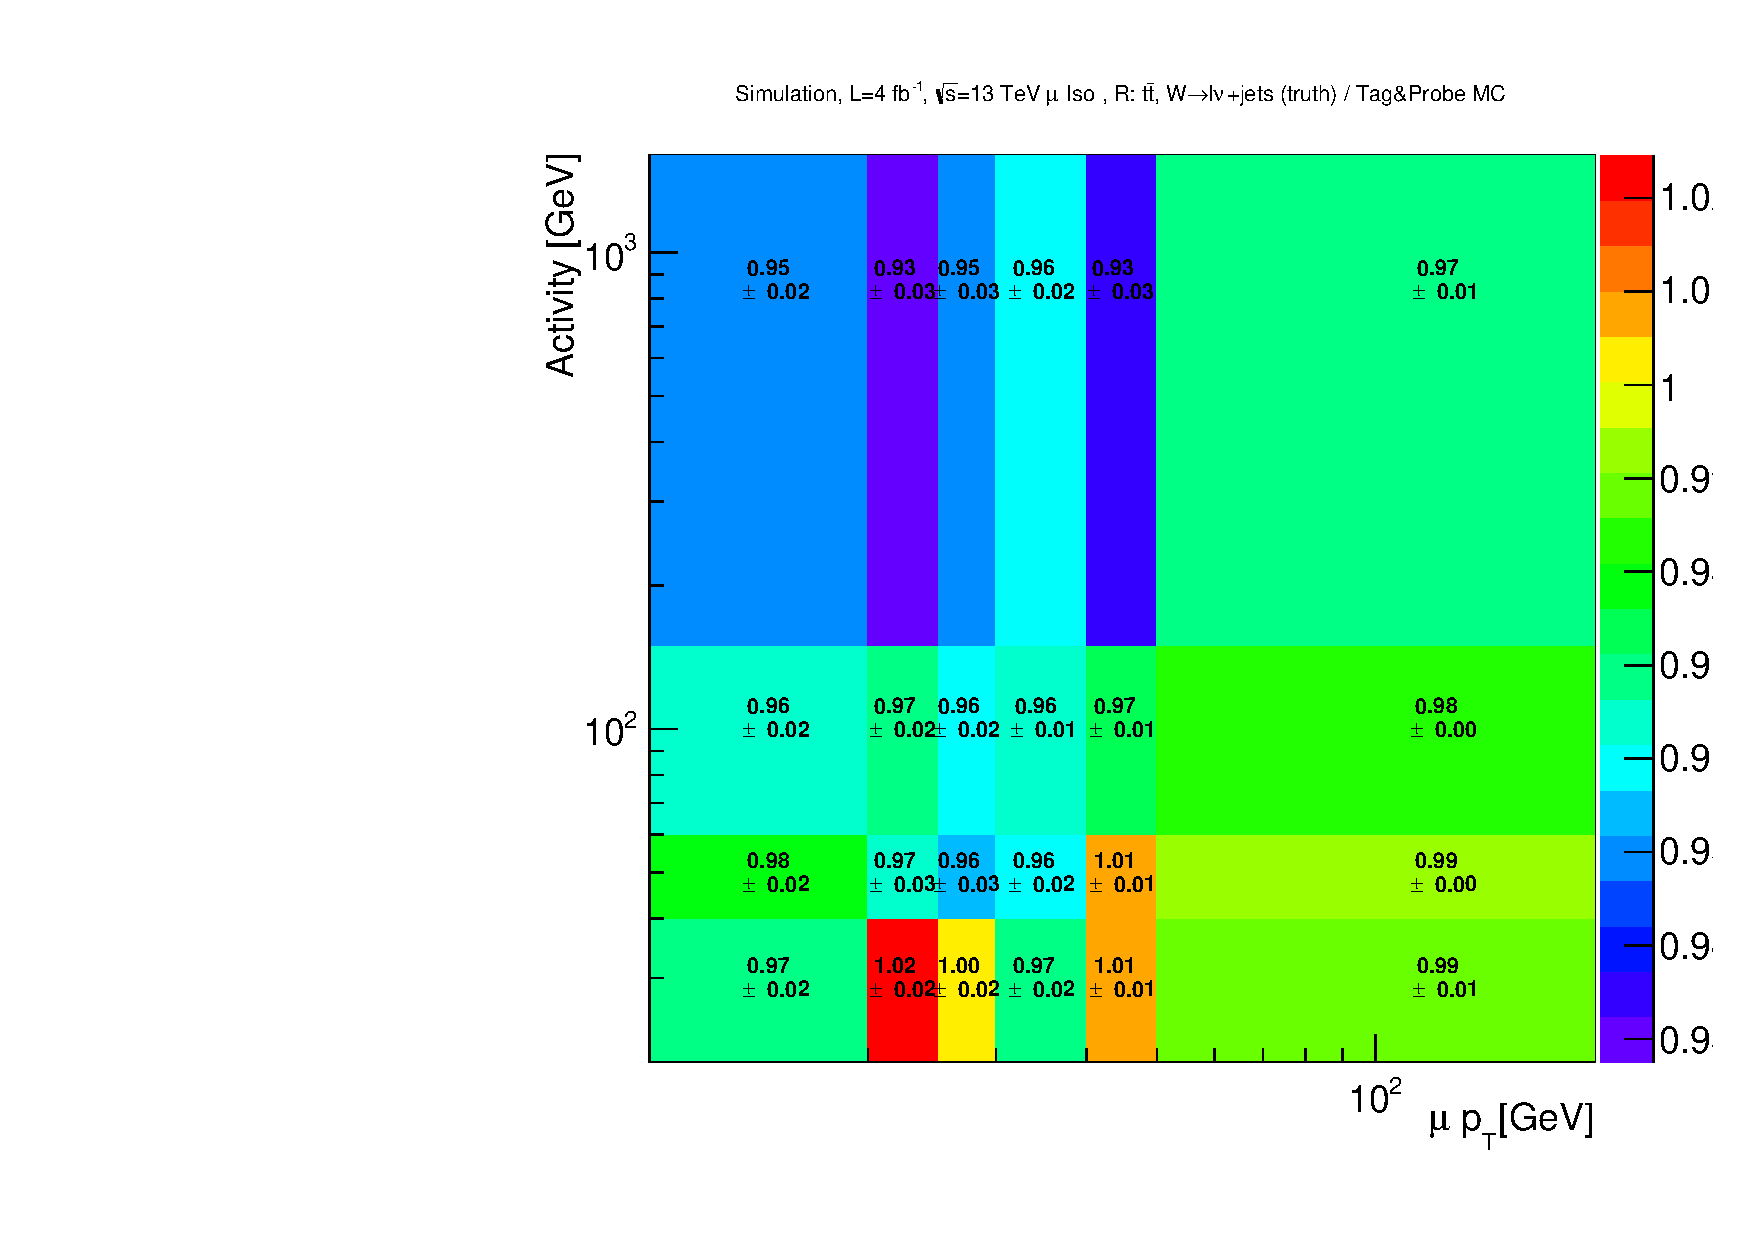
\includegraphics[width=1.\textwidth]{figures/efficiencies/tagandprobe/MuIsoPTActivity_ratio.pdf}};
    \begin{scope}[x={(image.south east)},y={(image.north west)}]
%         \draw[red,ultra thick,rounded corners] (0.62,0.65) rectangle (0.78,0.75);
%         \draw[red,ultra thick,rounded corners] (0.60,0.01) rectangle (0.75,0.99); % cordinates unten links(x,y) oben rechts(x,y)
    \end{scope}
   \end{tikzpicture}
   \end{column}
  \end{columns}
\begin{itemize}
 \item Good agreement between \ttbar \& \wpj \& Tag\&Probe $\mu$ isolation efficiencies! 
 \item Tag\&Probe are always slightly above \ttbar \& \wpj eff.
\end{itemize}

\end{frame}


\begin{frame}
 \frametitle{e Isolation Efficiencies}
  \begin{columns}

   \begin{column}{0.33\textwidth}
     \begin{itemize}
   \item e Iso \ttbar \& \wpj eff.
  \end{itemize}
    \begin{tikzpicture}
    \node[anchor=south west,inner sep=0] (image) at (0,0) {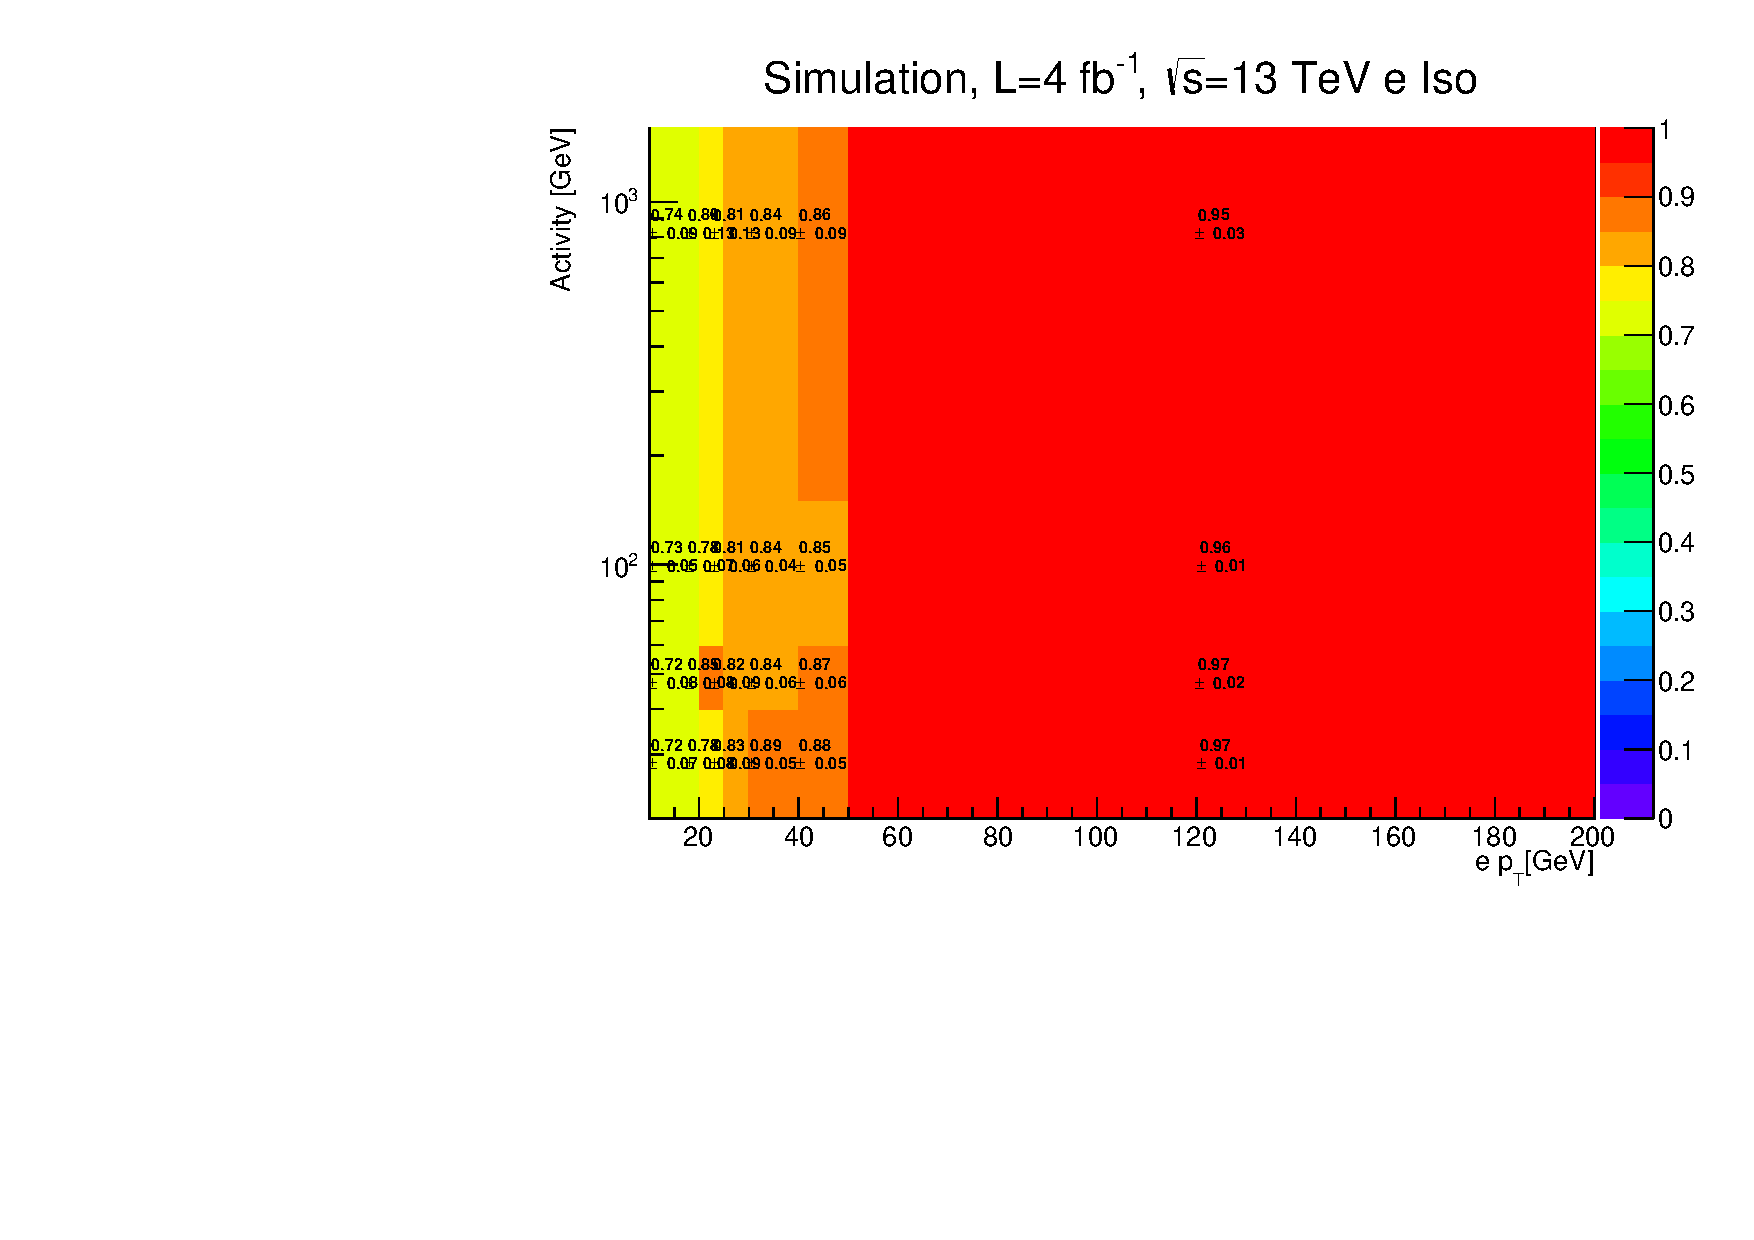
\includegraphics[width=1.\textwidth]{figures/efficiencies/ttbar-wpj/ElecIsoPTActivity.pdf}};
    \begin{scope}[x={(image.south east)},y={(image.north west)}]
%         \draw[red,ultra thick,rounded corners] (0.62,0.65) rectangle (0.78,0.75);
%         \draw[red,ultra thick,rounded corners] (0.60,0.01) rectangle (0.75,0.99); % cordinates unten links(x,y) oben rechts(x,y)
    \end{scope}
   \end{tikzpicture}
   \end{column}
   \begin{column}{0.33\textwidth}
   \begin{itemize}
    \item e Iso Tag \& Probe eff.
   \end{itemize}

    \begin{tikzpicture}
    \node[anchor=south west,inner sep=0] (image) at (0,0) {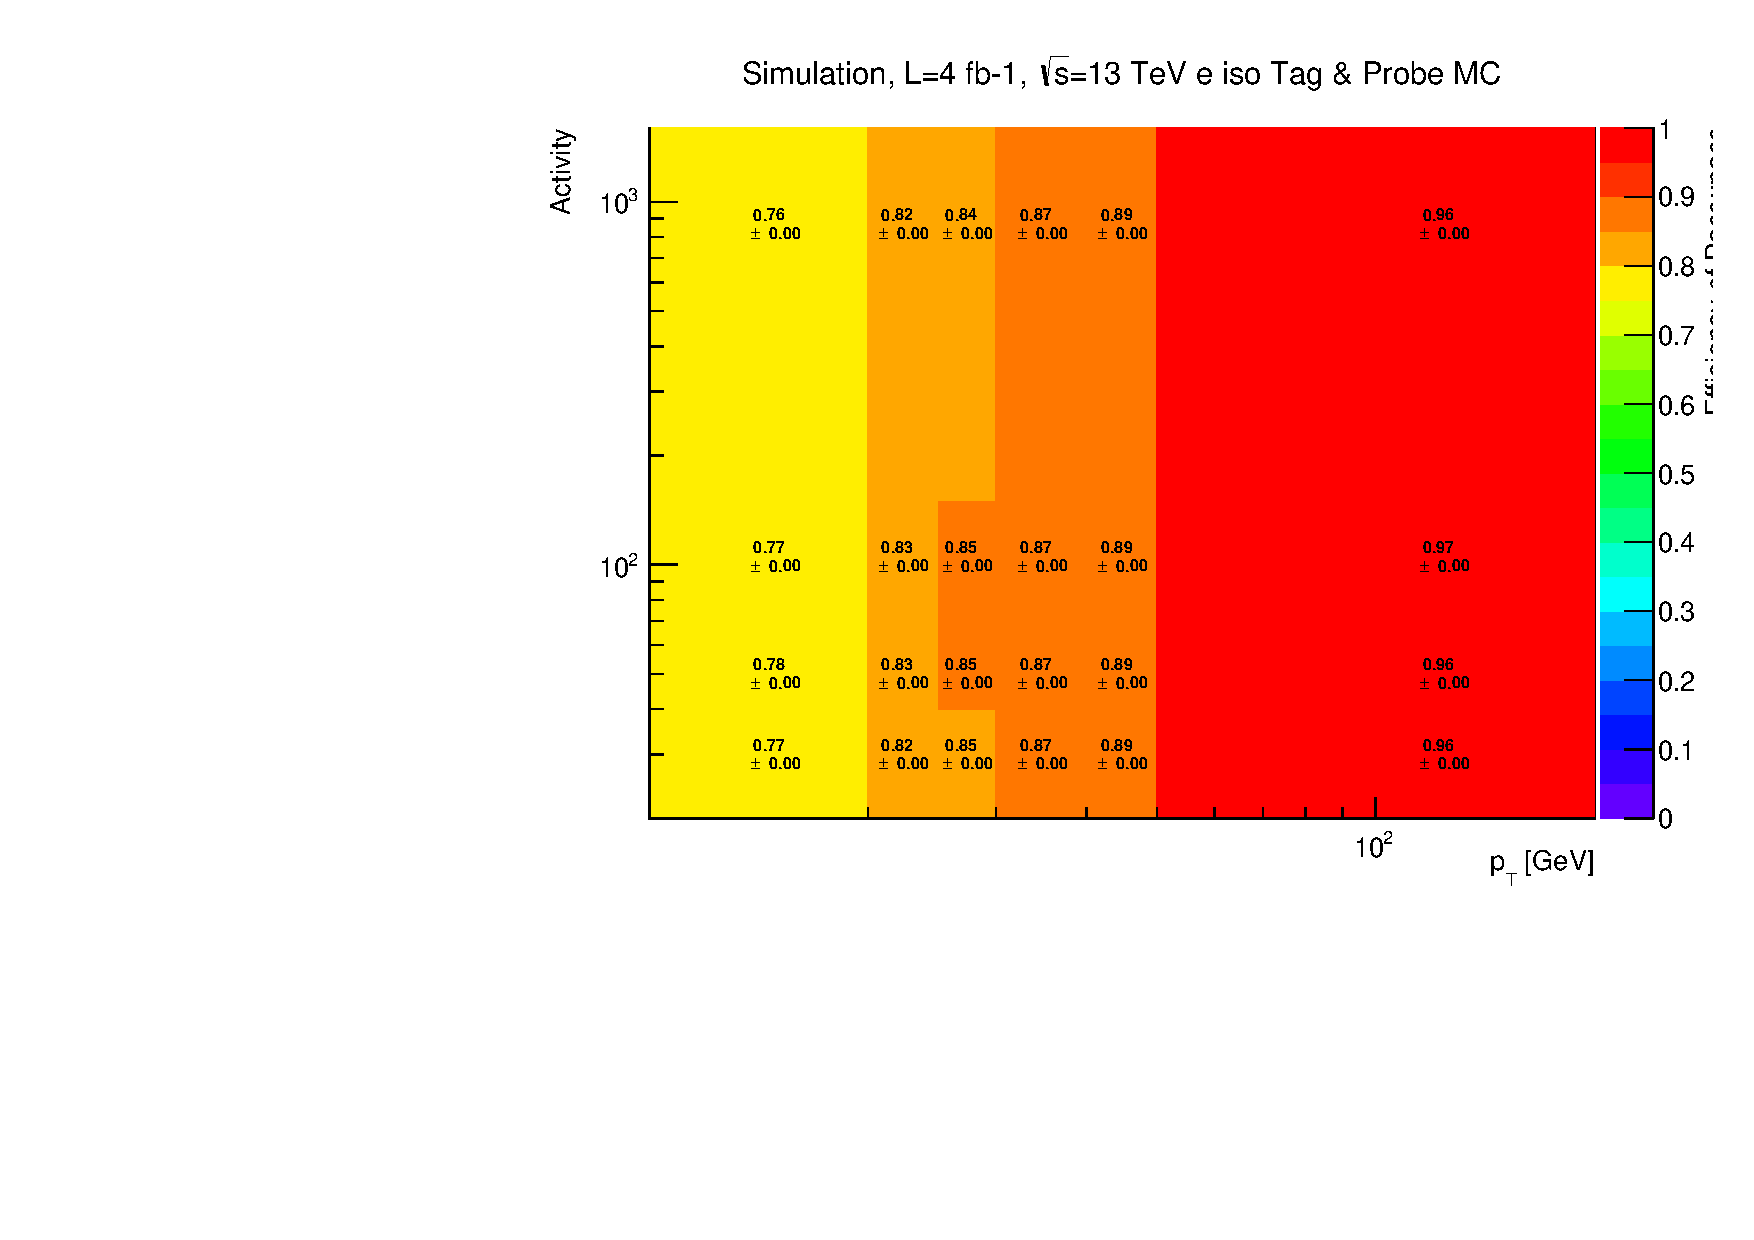
\includegraphics[width=1.\textwidth]{figures/efficiencies/tagandprobe/ElecIsoTagAndProbeMC.pdf}};
    \begin{scope}[x={(image.south east)},y={(image.north west)}]
%         \draw[red,ultra thick,rounded corners] (0.62,0.65) rectangle (0.78,0.75);
%         \draw[red,ultra thick,rounded corners] (0.60,0.01) rectangle (0.75,0.99); % cordinates unten links(x,y) oben rechts(x,y)
    \end{scope}
   \end{tikzpicture}
   \end{column}
   \begin{column}{0.33\textwidth}
   \begin{itemize}
    \item Ratio: \ttbar \& \wpj / Tag \& Probe eff.
   \end{itemize}

    \begin{tikzpicture}
    \node[anchor=south west,inner sep=0] (image) at (0,0) {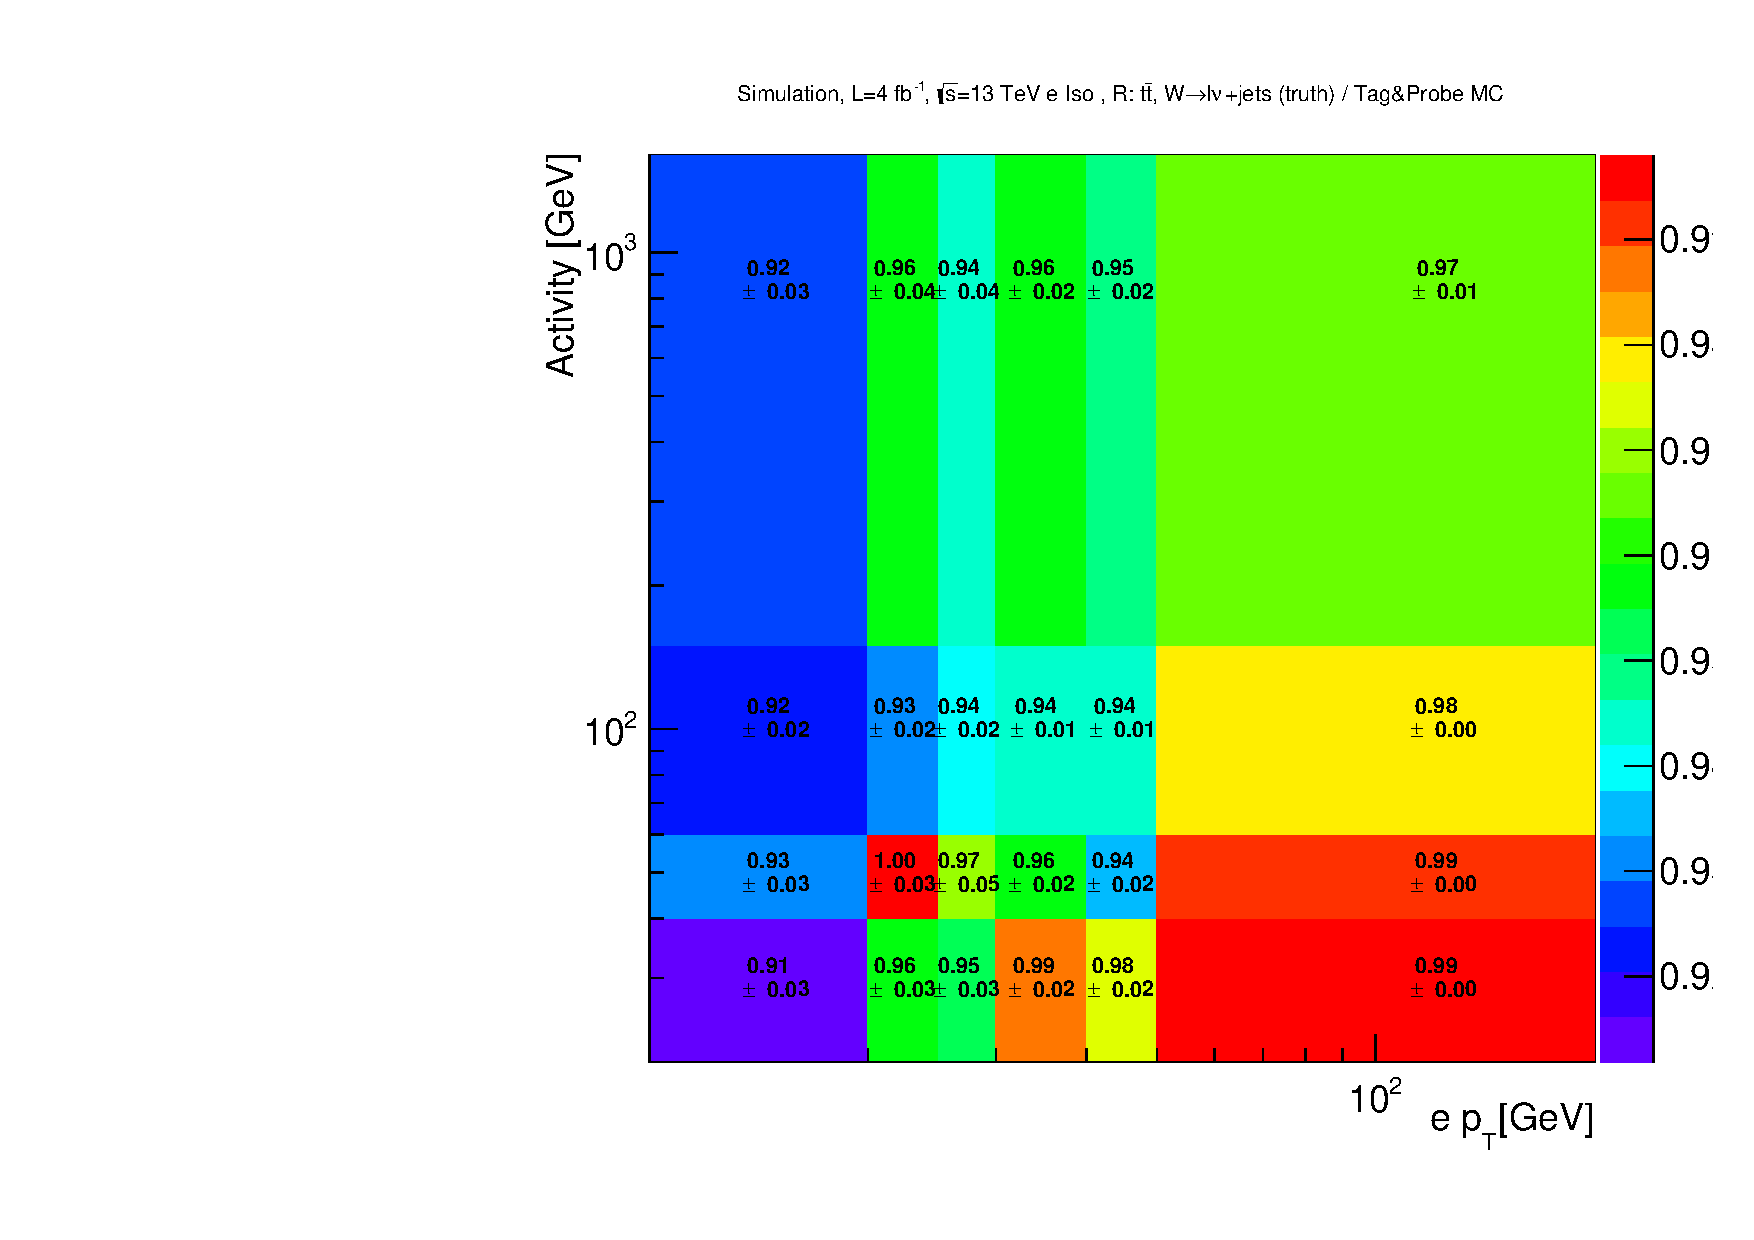
\includegraphics[width=1.\textwidth]{figures/efficiencies/tagandprobe/ElecIsoPTActivity_ratio.pdf}};
    \begin{scope}[x={(image.south east)},y={(image.north west)}]
%         \draw[red,ultra thick,rounded corners] (0.62,0.65) rectangle (0.78,0.75);
%         \draw[red,ultra thick,rounded corners] (0.60,0.01) rectangle (0.75,0.99); % cordinates unten links(x,y) oben rechts(x,y)
    \end{scope}
   \end{tikzpicture}
   \end{column}
  \end{columns}
\begin{itemize}
 \item Good agreement between \ttbar \& \wpj \& Tag\&Probe e isolation efficiencies! 
 \item Tag\&Probe are always slightly above \ttbar \& \wpj eff.
\end{itemize}

\end{frame}

\begin{frame}
 \frametitle{Reconstruction \& ID validation}
 
   \begin{columns}
 \begin{column}{0.50\textwidth}
 
   \begin{itemize}
  \item We compute our combined reco/ID eff using gen information:
  \begin{itemize}
   \item Reco/ID Eff.: Select events with prompt lepton $\rightarrow$ Ask for $\pt>10\gev$ \& $|\eta|<2.5(2.4)$ (on gen) $\rightarrow$ try to match well reconstructed and ID lepton (on reco level) $eff.=p/(p+f)$
  \end{itemize}
  \item Tag\&Probe Difficultiy: 
  \item No gen info available. Test object selected on reco level. Most basic object desirable (avoid gab see above).
  \end{itemize}
 \end{column}
  \begin{column}{0.50\textwidth}
\begin{tikzpicture}
    \node[anchor=south west,inner sep=0] (image) at (0,0) {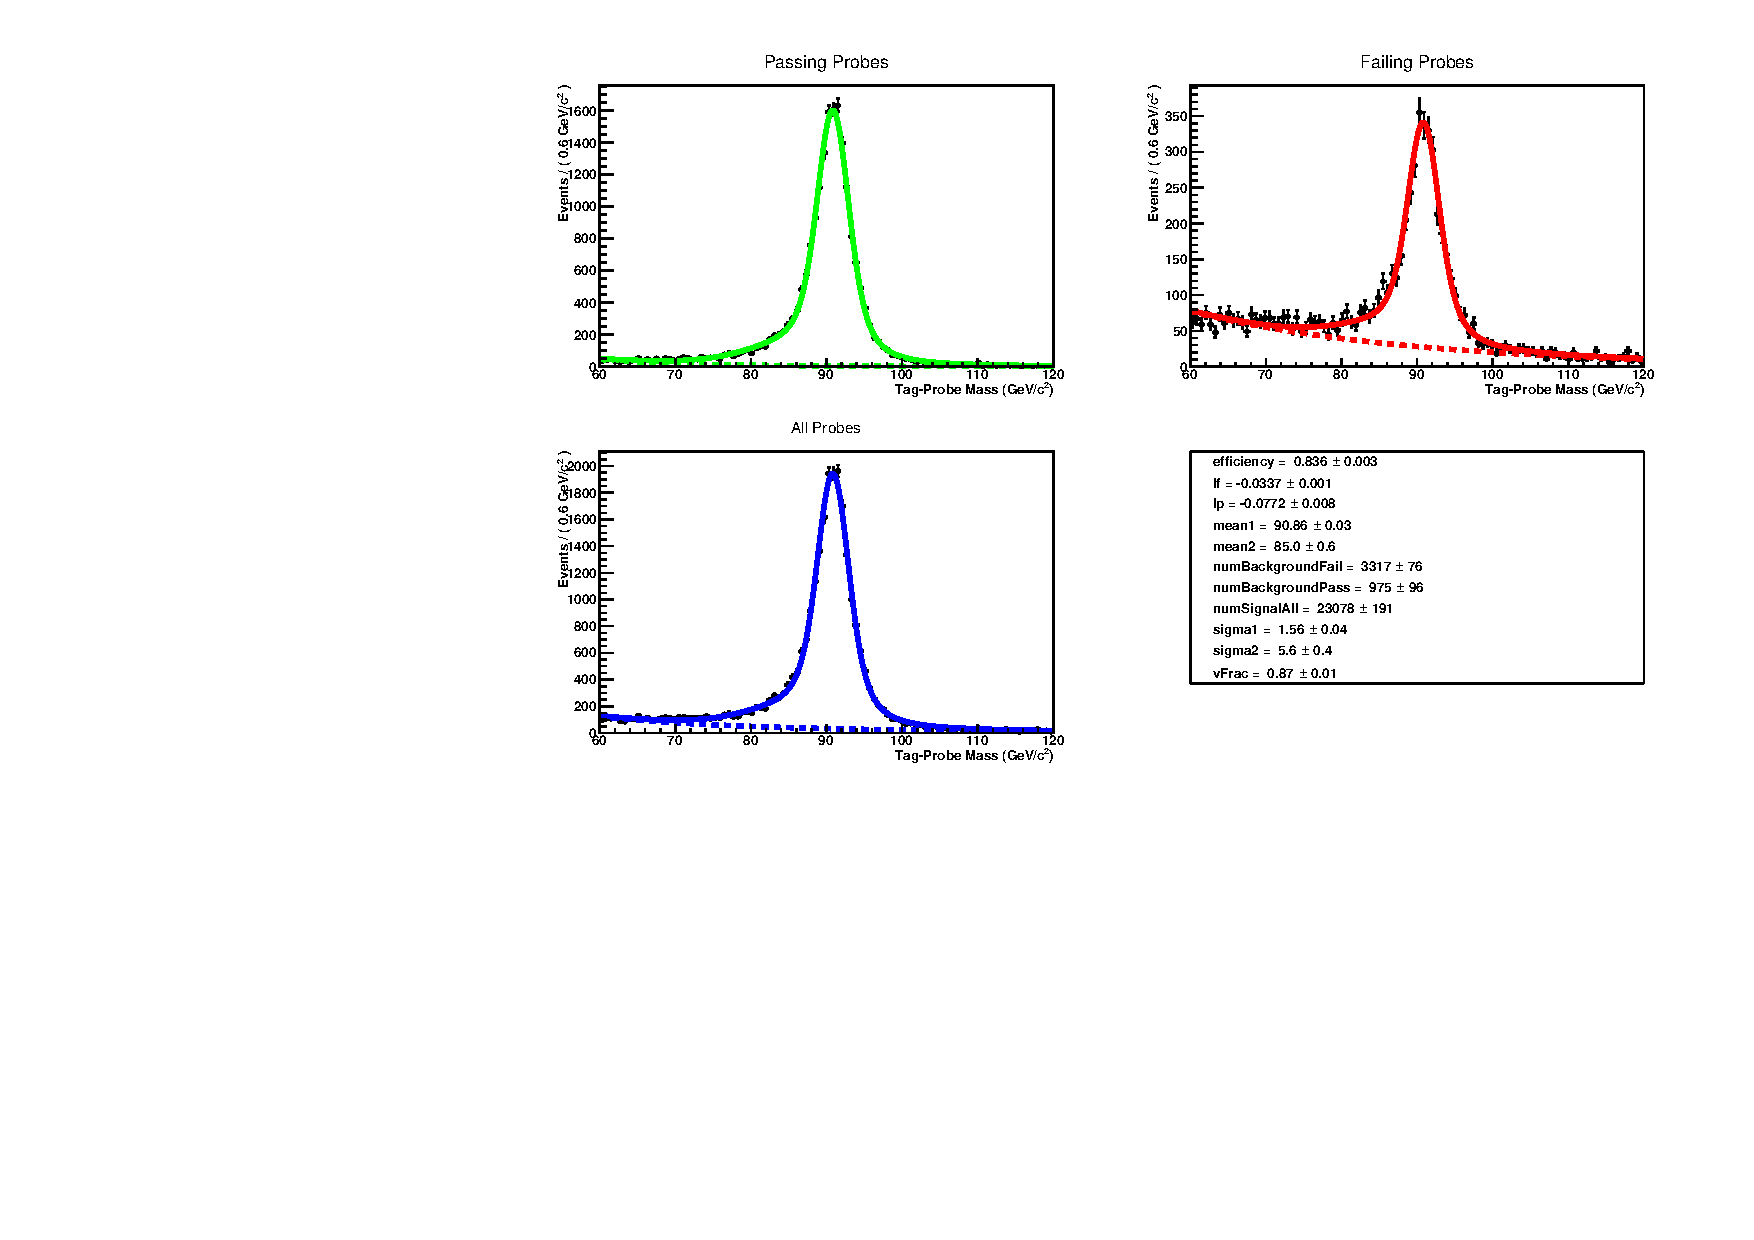
\includegraphics[width=1.\textwidth]{figures/efficiencies/tagandprobe/MuIso_Example_TagAndProbe_Fit.pdf}};
    \begin{scope}[x={(image.south east)},y={(image.north west)}]
%         \draw[red,ultra thick,rounded corners] (0.62,0.65) rectangle (0.78,0.75);
    \end{scope}
\end{tikzpicture}  
\begin{itemize}
 \item BUT need to keep ratio Z mass signal over bkg reasonable for fit! Especially in failing collection!
 \item $Eff. = p / (p + f)$  
\end{itemize}
  \end{column}
 \end{columns}
\end{frame}
\begin{frame}
 \frametitle{Reconstruction \& ID Tag\&Probe Setup}
 
 Setup:
 \begin{itemize}
  \item Tag: Isolated $\mu/e$
  \item Probe:
  \begin{itemize}
   \item $\mu$: miniAOD slimmedMuon; Gap: Missing muons within acceptance ($\pt>10\gev$ \& $|\eta|<2.4$)  that are NOT slimmedMuons\\ (most basic: tracker muons)
   \item $e$: miniAOD slimmedPhoton; Gap: Missing electrons within acceptance ($\pt>10\gev$ \& $|\eta|<2.5$) that are NOT Photons (especially in high Activity region) (most basic: superclusters)
  \end{itemize}
 \end{itemize}
\end{frame}
\begin{frame}
 \frametitle{$\mu$ Reconstruction/ID Efficiencies}
  \begin{columns}

   \begin{column}{0.33\textwidth}
     \begin{itemize}
   \item $\mu$ Reco/ID \ttbar \& \wpj eff.
  \end{itemize}
    \begin{tikzpicture}
    \node[anchor=south west,inner sep=0] (image) at (0,0) {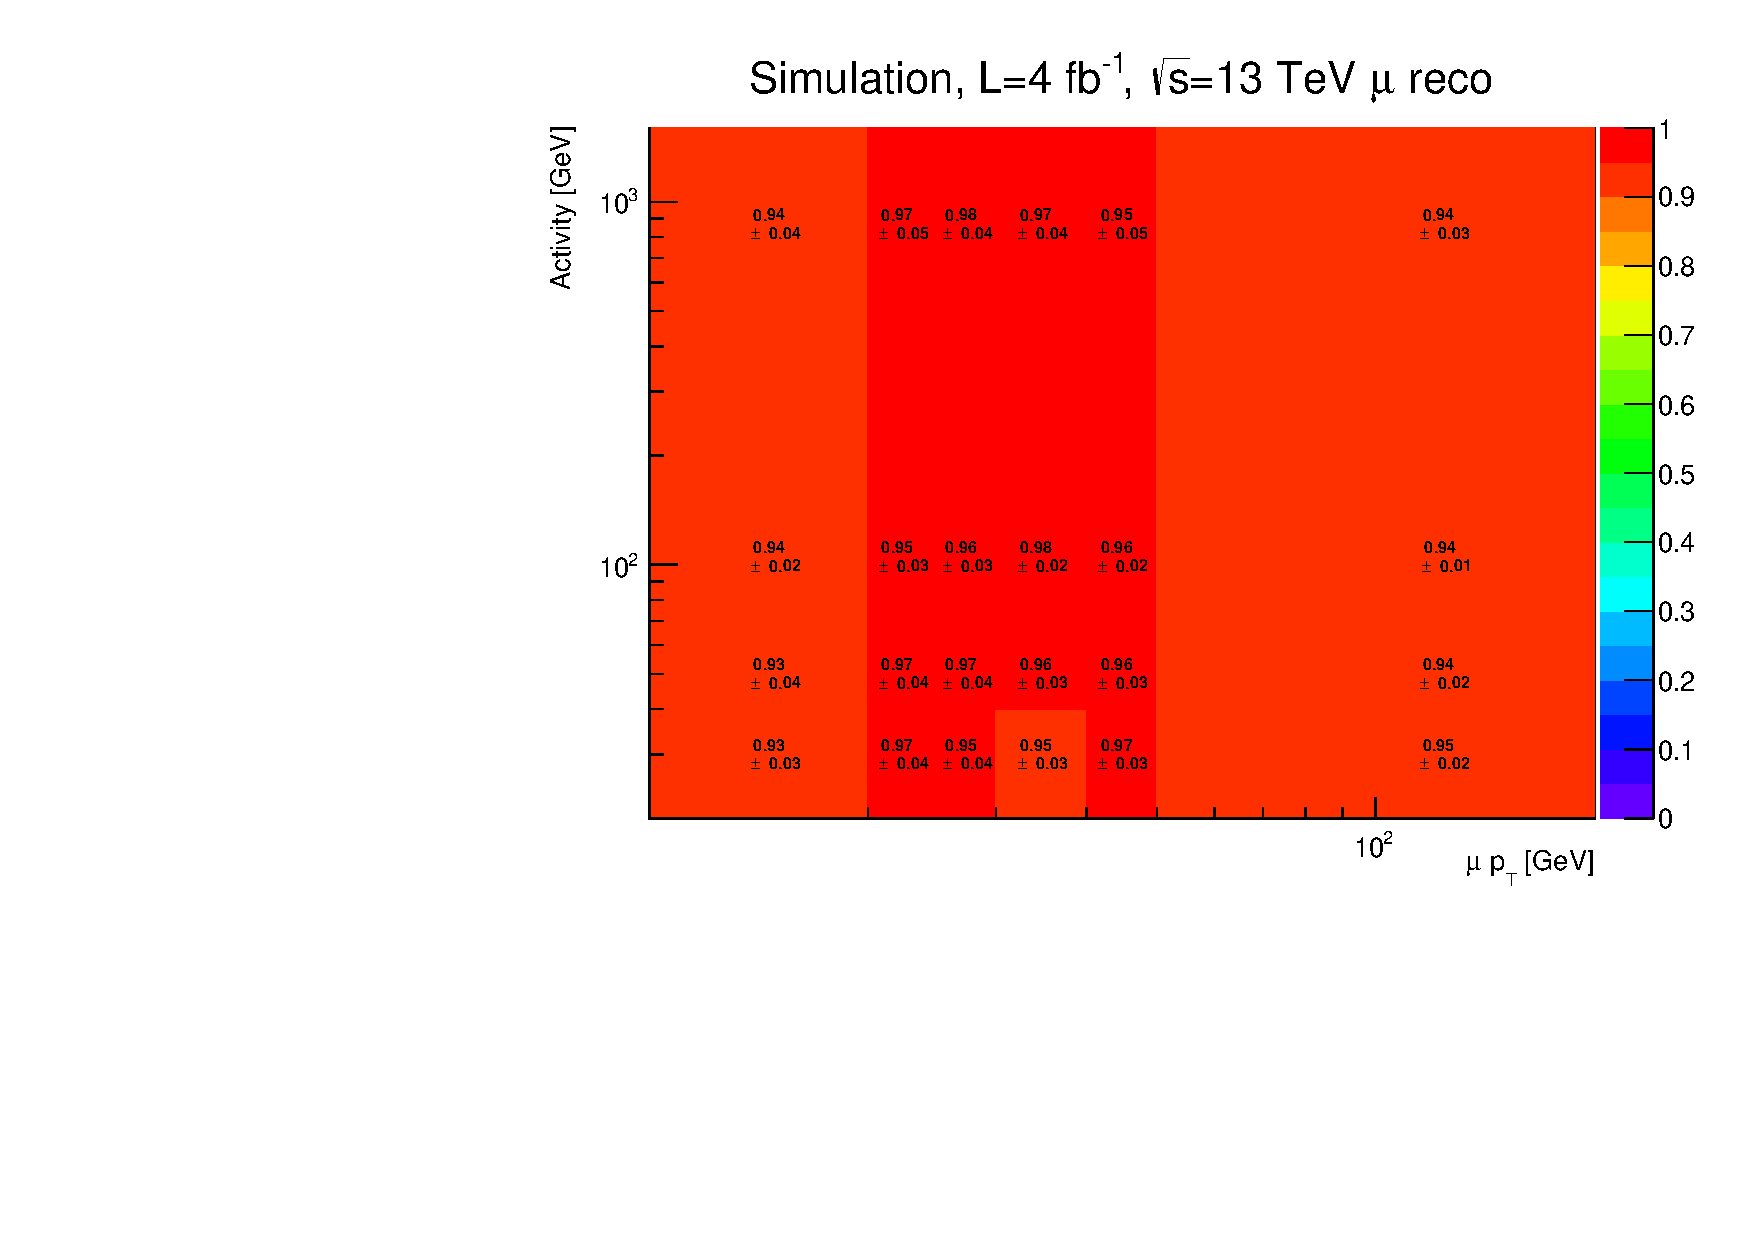
\includegraphics[width=1.\textwidth]{figures/efficiencies/ttbar-wpj/MuRecoPTActivity.pdf}};
    \begin{scope}[x={(image.south east)},y={(image.north west)}]
%         \draw[red,ultra thick,rounded corners] (0.62,0.65) rectangle (0.78,0.75);
%         \draw[red,ultra thick,rounded corners] (0.60,0.01) rectangle (0.75,0.99); % cordinates unten links(x,y) oben rechts(x,y)
    \end{scope}
   \end{tikzpicture}
   \end{column}
   \begin{column}{0.33\textwidth}
   \begin{itemize}
    \item $\mu$ Reco/ID Tag \& Probe eff.
   \end{itemize}

    \begin{tikzpicture}
    \node[anchor=south west,inner sep=0] (image) at (0,0) {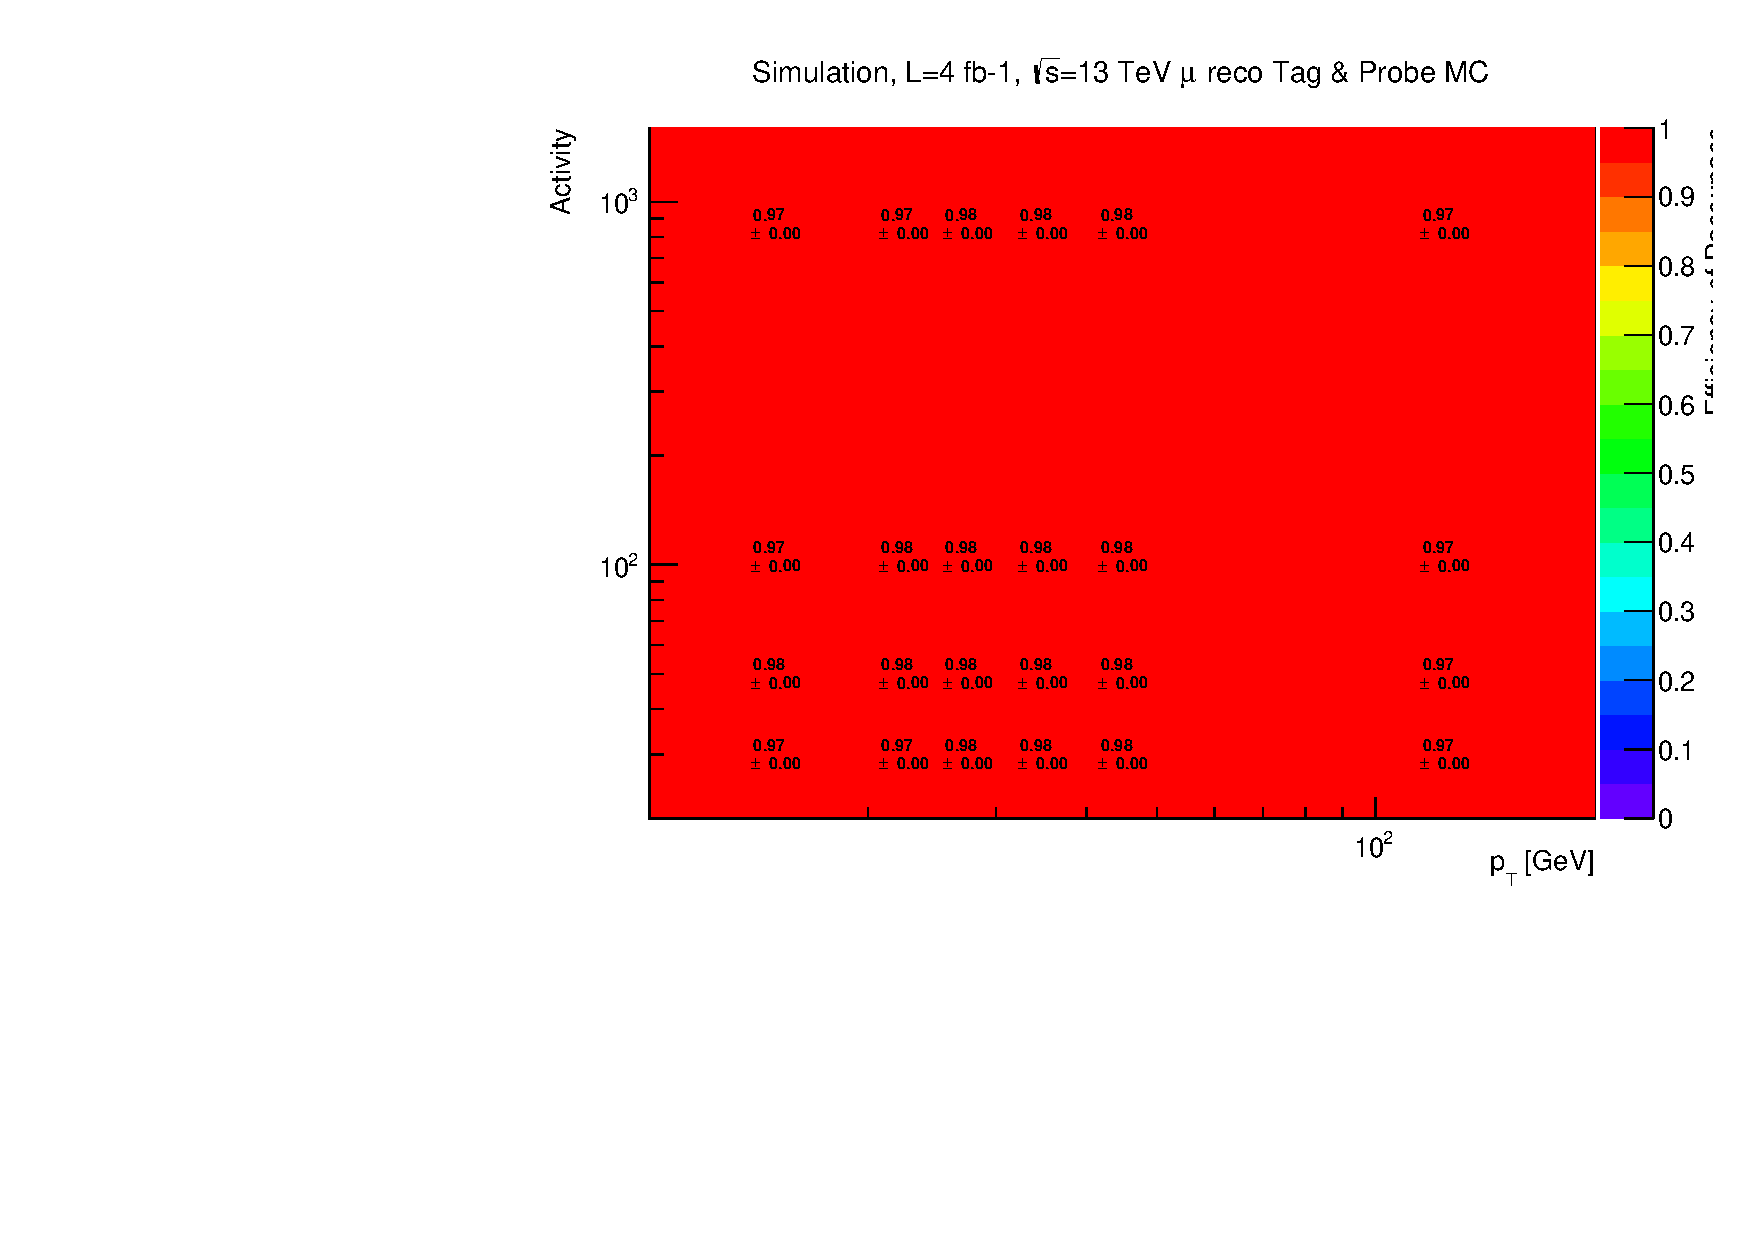
\includegraphics[width=1.\textwidth]{figures/efficiencies/tagandprobe/MuRecoTagAndProbeMC.pdf}};
    \begin{scope}[x={(image.south east)},y={(image.north west)}]
%         \draw[red,ultra thick,rounded corners] (0.62,0.65) rectangle (0.78,0.75);
%         \draw[red,ultra thick,rounded corners] (0.60,0.01) rectangle (0.75,0.99); % cordinates unten links(x,y) oben rechts(x,y)
    \end{scope}
   \end{tikzpicture}
   \end{column}
   \begin{column}{0.33\textwidth}
   \begin{itemize}
    \item Ratio: \ttbar \& \wpj / Tag \& Probe eff.
   \end{itemize}

    \begin{tikzpicture}
    \node[anchor=south west,inner sep=0] (image) at (0,0) {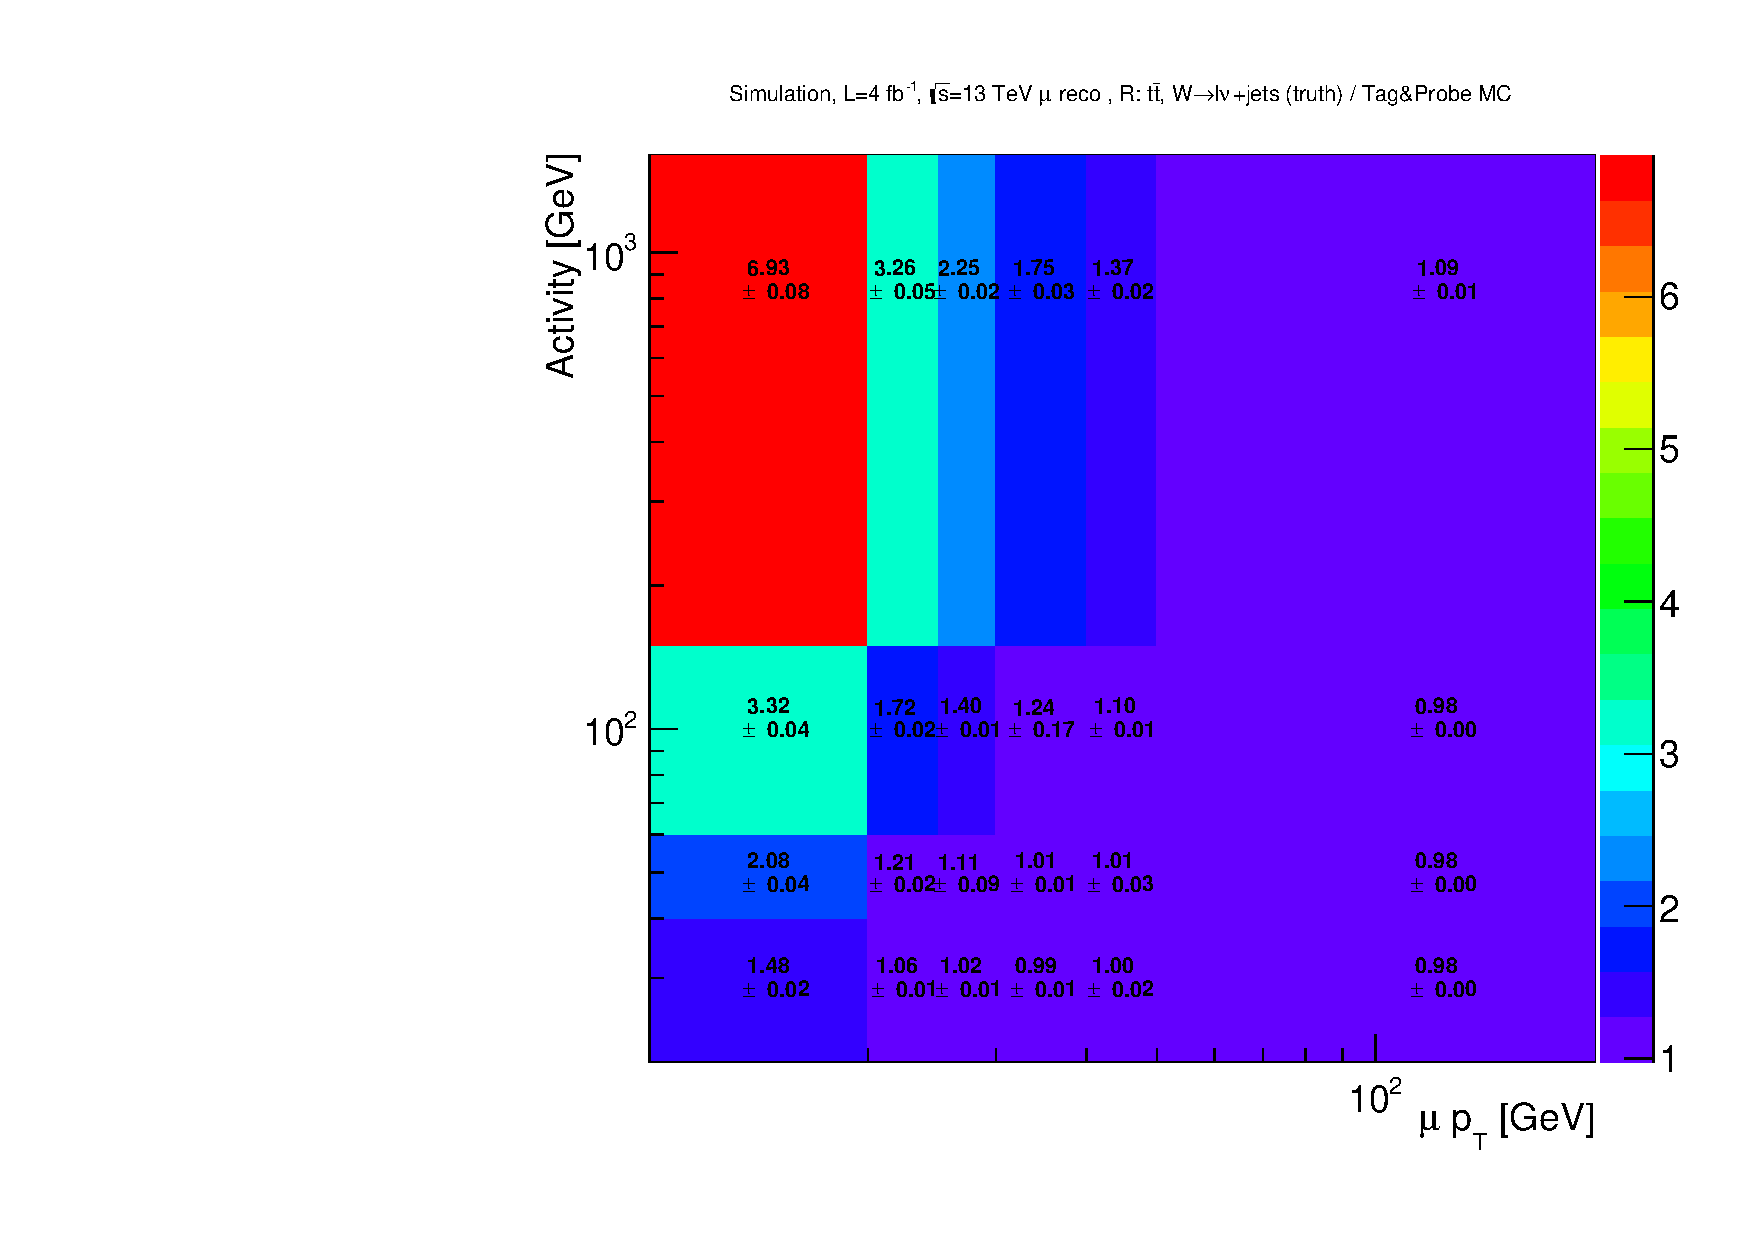
\includegraphics[width=1.\textwidth]{figures/efficiencies/tagandprobe/MuRecoPTActivity_ratio.pdf}};
    \begin{scope}[x={(image.south east)},y={(image.north west)}]
%         \draw[red,ultra thick,rounded corners] (0.62,0.65) rectangle (0.78,0.75);
%         \draw[red,ultra thick,rounded corners] (0.60,0.01) rectangle (0.75,0.99); % cordinates unten links(x,y) oben rechts(x,y)
    \end{scope}
   \end{tikzpicture}
   \end{column}
  \end{columns}
\begin{itemize}
 \item Overall the expected higher efficiencies can be observed in Tag\&Probe due to the gab of probe object (slimmedMuon) and all muons within acceptance
\end{itemize}

\end{frame}


\begin{frame}
 \frametitle{e Reconstruction/ID Efficiencies}
  \begin{columns}

   \begin{column}{0.33\textwidth}
     \begin{itemize}
   \item e Reco/ID \ttbar \& \wpj eff.
  \end{itemize}
    \begin{tikzpicture}
    \node[anchor=south west,inner sep=0] (image) at (0,0) {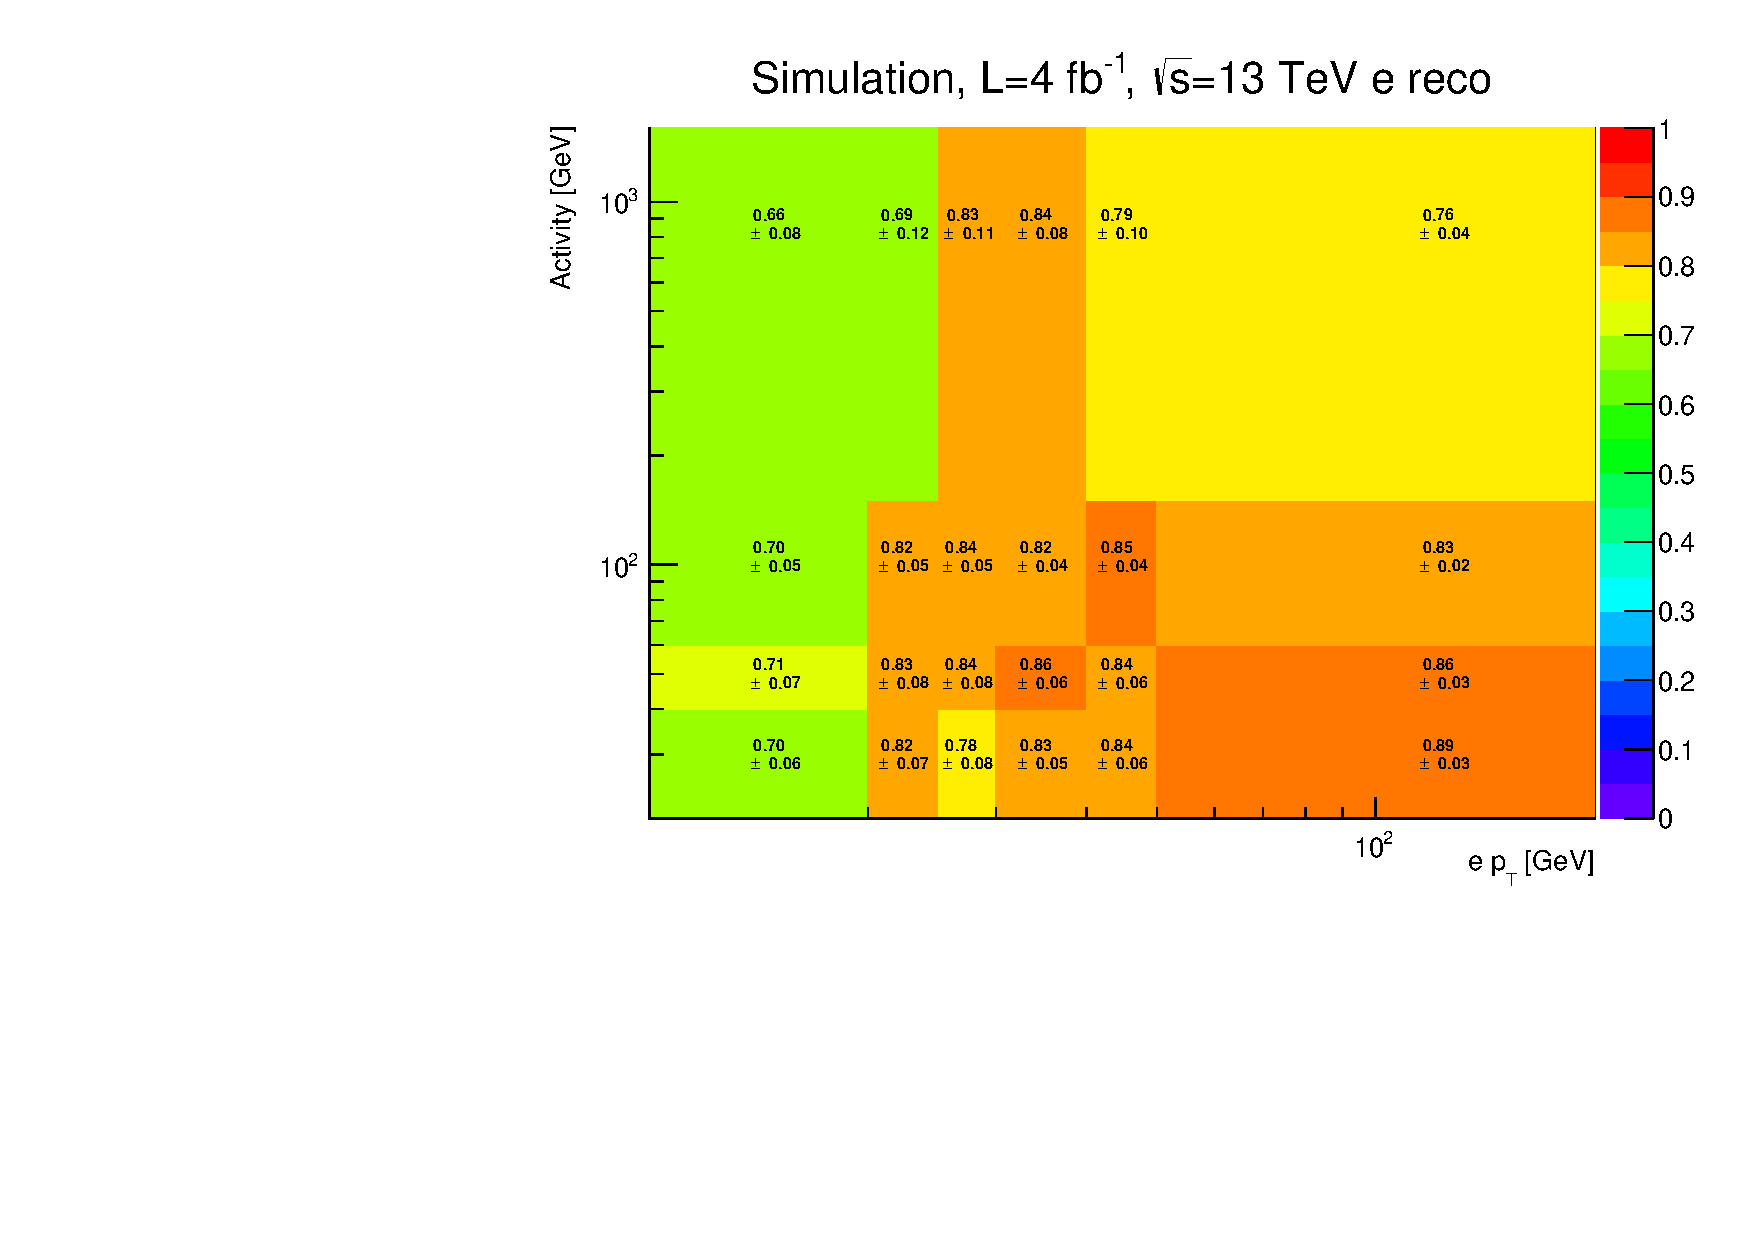
\includegraphics[width=1.\textwidth]{figures/efficiencies/ttbar-wpj/ElecRecoPTActivity.pdf}};
    \begin{scope}[x={(image.south east)},y={(image.north west)}]
%         \draw[red,ultra thick,rounded corners] (0.62,0.65) rectangle (0.78,0.75);
%         \draw[red,ultra thick,rounded corners] (0.60,0.01) rectangle (0.75,0.99); % cordinates unten links(x,y) oben rechts(x,y)
    \end{scope}
   \end{tikzpicture}
   \end{column}
   \begin{column}{0.33\textwidth}
   \begin{itemize}
    \item e Reco/ID Tag \& Probe eff.
   \end{itemize}

    \begin{tikzpicture}
    \node[anchor=south west,inner sep=0] (image) at (0,0) {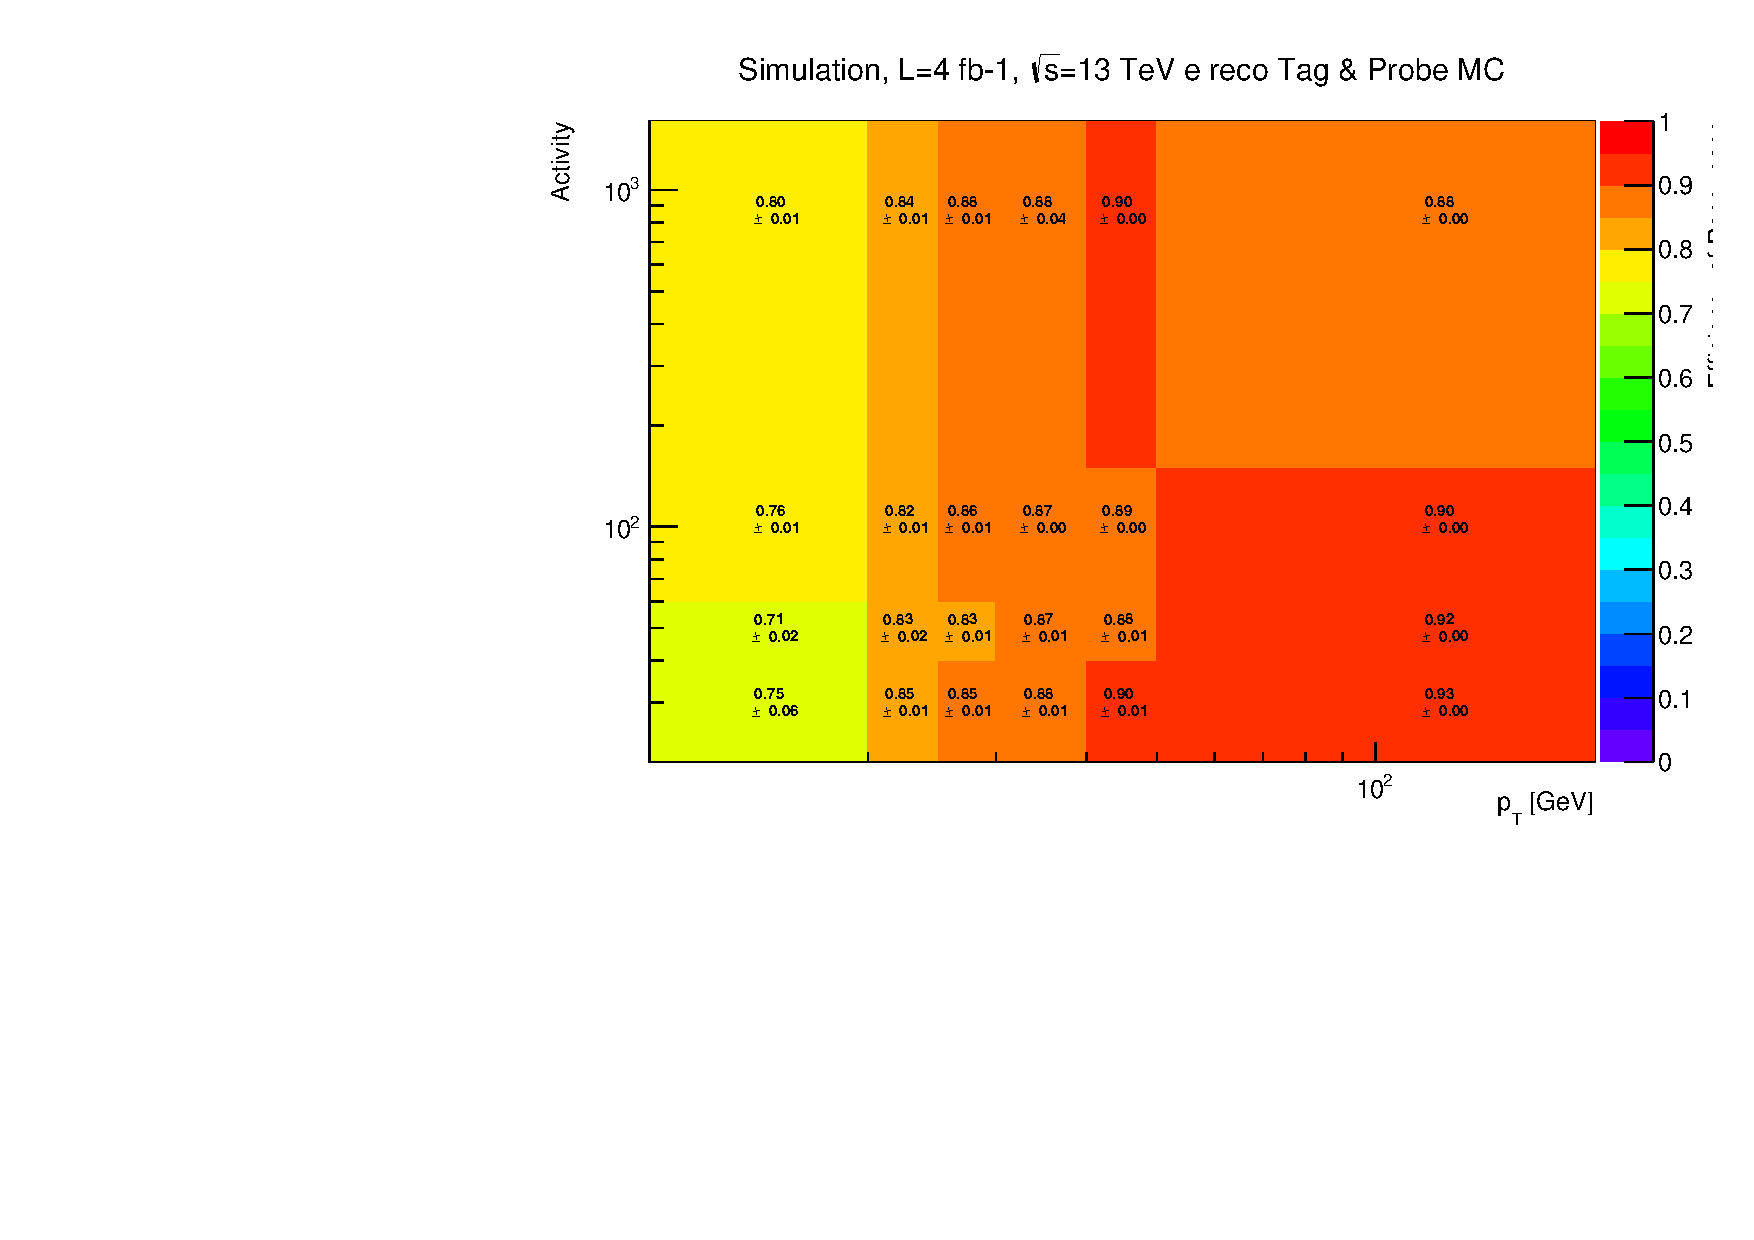
\includegraphics[width=1.\textwidth]{figures/efficiencies/tagandprobe/ElecRecoTagAndProbeMC.pdf}};
    \begin{scope}[x={(image.south east)},y={(image.north west)}]
%         \draw[red,ultra thick,rounded corners] (0.62,0.65) rectangle (0.78,0.75);
%         \draw[red,ultra thick,rounded corners] (0.60,0.01) rectangle (0.75,0.99); % cordinates unten links(x,y) oben rechts(x,y)
    \end{scope}
   \end{tikzpicture}
   \end{column}
   \begin{column}{0.33\textwidth}
   \begin{itemize}
    \item Ratio: \ttbar \& \wpj / Tag \& Probe eff.
   \end{itemize}

    \begin{tikzpicture}
    \node[anchor=south west,inner sep=0] (image) at (0,0) {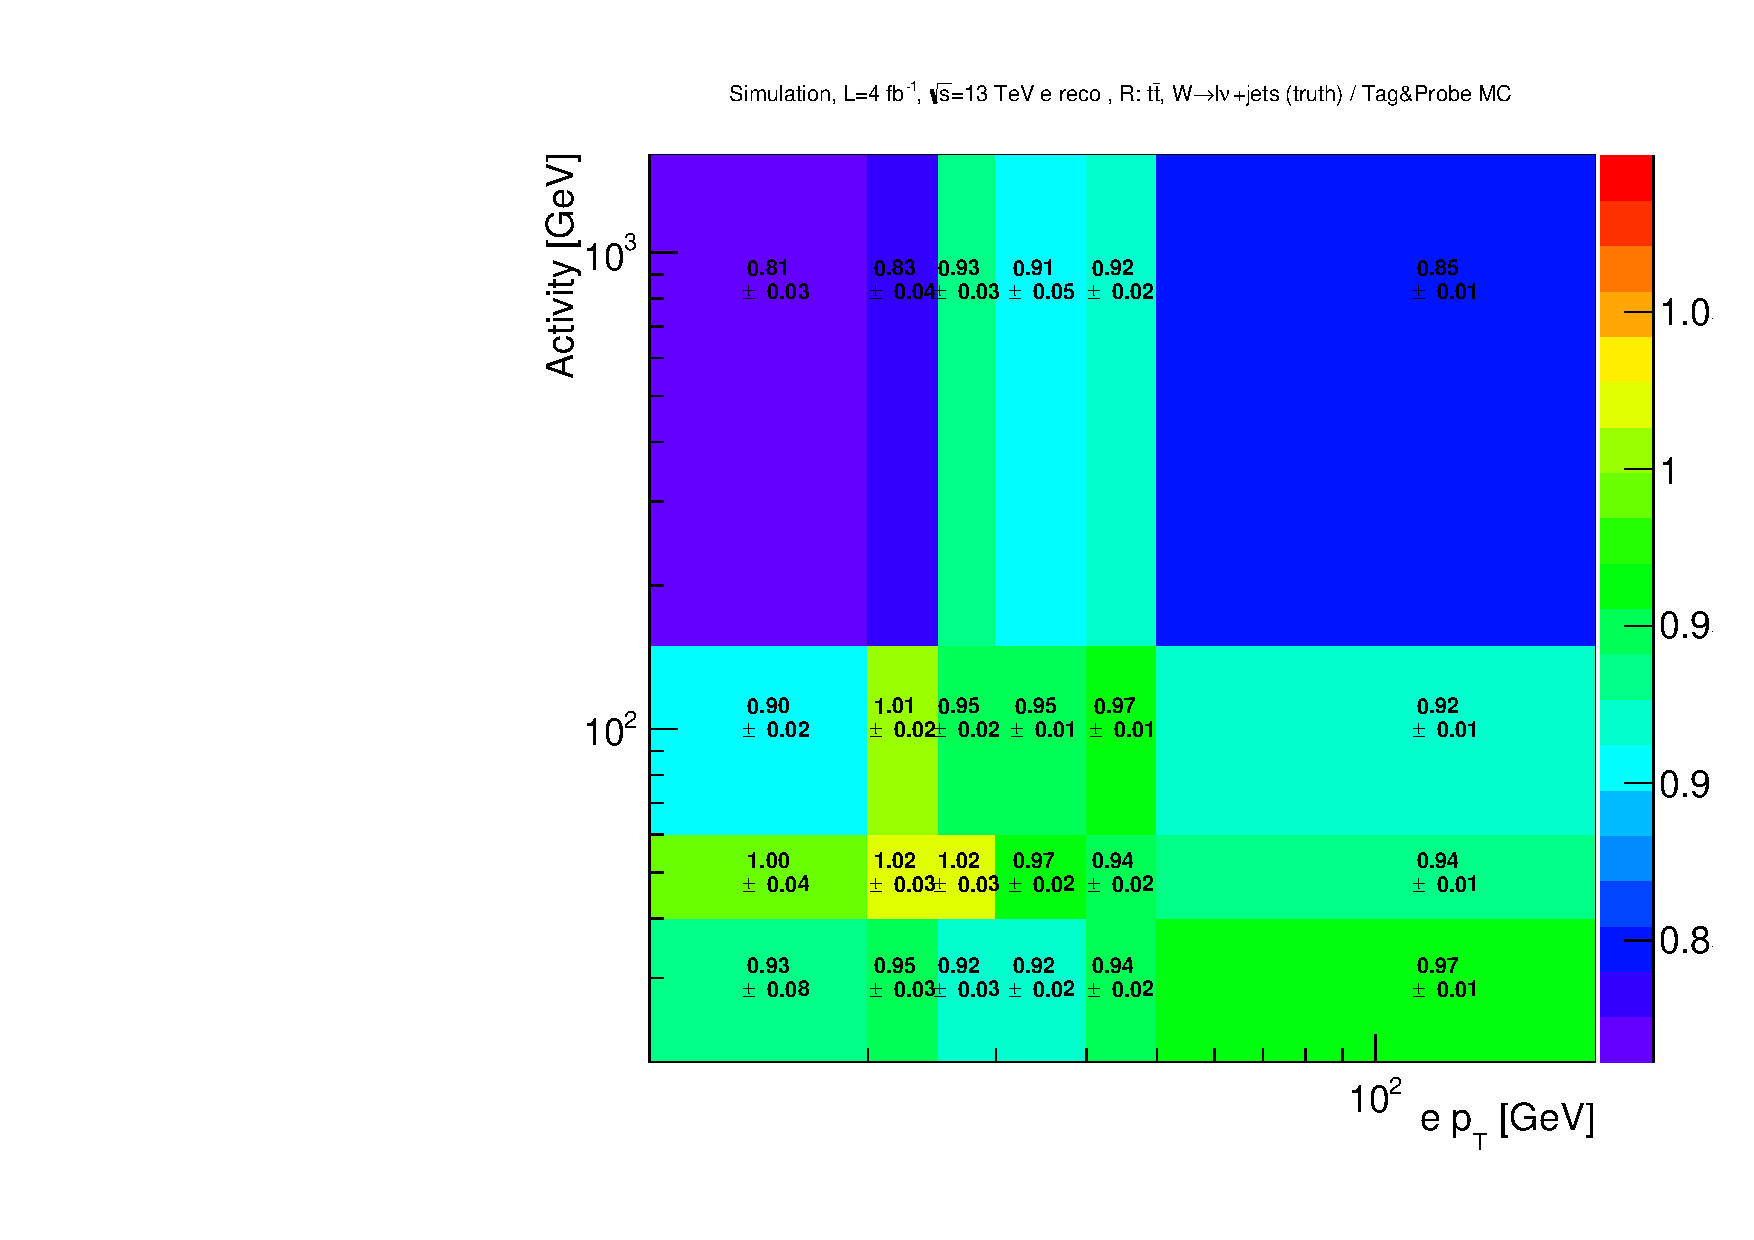
\includegraphics[width=1.\textwidth]{figures/efficiencies/tagandprobe/ElecRecoPTActivity_ratio.pdf}};
    \begin{scope}[x={(image.south east)},y={(image.north west)}]
%         \draw[red,ultra thick,rounded corners] (0.62,0.65) rectangle (0.78,0.75);
%         \draw[red,ultra thick,rounded corners] (0.60,0.01) rectangle (0.75,0.99); % cordinates unten links(x,y) oben rechts(x,y)
    \end{scope}
   \end{tikzpicture}
   \end{column}
  \end{columns}
\begin{itemize}
 \item At high $\pt$ to Activity ratio good agreement. Increasing activity increases probability to lose already probe object (photon) biases to higher eff in Tag\&Probe. Also $\pt$ threshold of Probe objects at 15\gev.
\end{itemize}

\end{frame}


\begin{frame}
 \begin{block}{}
 \centering
 \Large Tack\&Probe:\\Isolated $e,\mu,\pi$ tracks Studies
 \end{block}
\end{frame}


\subsection{Concept}
\begin{frame}
\frametitle{Iso Track Reduction}
 \begin{center}
\begin{tikzpicture}
    \node[anchor=south west,inner sep=0] (image) at (0,0) {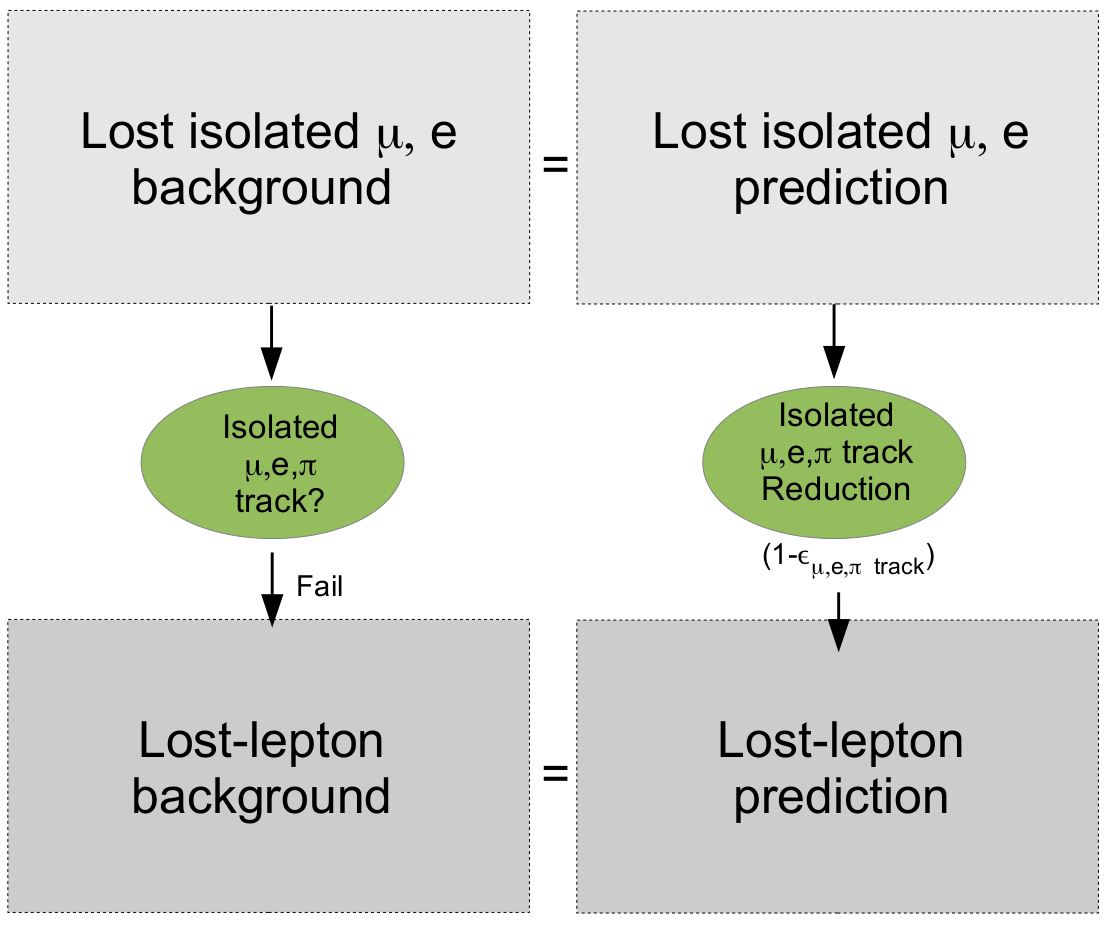
\includegraphics[width=0.5\textwidth]{figures/Sketches/LostLeptonSketch_Prediction_IsoTrackReduction_small.png}};
    \begin{scope}[x={(image.south east)},y={(image.north west)}]
%         \draw[red,ultra thick,rounded corners] (0.62,0.65) rectangle (0.78,0.75);
%         \draw[red,ultra thick,rounded corners] (0.60,0.01) rectangle (0.75,0.99); % coordinates unten links(x,y) oben rechts(x,y)
%             \draw[blue,ultra thick,rounded corners] (0.40,0.01) rectangle (0.55,0.99); % coordinates unten links(x,y) oben rechts(x,y)
    \end{scope}
\end{tikzpicture}
 \end{center}
 \begin{itemize}
  \item Correction factor is split up in: $\epsilon_{track} = \epsilon_{\mu} +\epsilon_{e} +\epsilon_{\pi} $ where $\epsilon_{\pi}$ contains $\mu/e$ that fail the pdgID assignment from PF algorithm
  \item Study these efficiencies using Tag and Probe
 \end{itemize}
\end{frame}
\begin{frame}
 \frametitle{Tag\&Probe Setup}
\begin{itemize}
 \item Muon, Electron Tracks:
 \begin{itemize}
  \item Charged PFCand, $\pt>5 \gev, |\eta|<2.5$, $\mt<100 \gev$, ask for pdgID=11,13
  \item Iso: $\Sigma ( \pt\text(Tracks)\Delta R<0.3 )/(\pt Track) < 0.2$ (with $dz<0.1$)
 \end{itemize}
 \item Pion Tracks:
 \begin{itemize}
  \item Charged PFCand, $\pt>10 \gev, |\eta|<2.5$, $\mt<100 \gev$, ask for pdgID=211
  \item Iso: $\Sigma ( \pt\text(Tracks)\Delta R<0.3 )/(\pt Track) < 0.1$ (with $dz<0.1$)
 \end{itemize}
 \end{itemize}

 
\end{frame}

\begin{frame}
 \frametitle{Where do we apply the isolated Track veto?}
 \begin{itemize}
  \item Isolated track veto is applied on top of isolated lepton veto
  \begin{itemize}
   \item We are interested in the fraction of lost isolated electron and muon events which are selected by the isolated track veto
  \end{itemize}
  \item Rejection efficiency derived on simulated \ttbar \& \wpj events $\rightarrow$ applied to data
  \item Need to validate in data using Tag\&Probe
  \item Tag objects: Well isolated $\mu/e$
  \item Probe objects: Tracks within acceptance cuts with pdgID of $\mu/e$ applied by PF algorithm. Leaving two gabs:
  \begin{itemize}
   \item Can not account of  $\mu/e$  failing pdgID assignment
   \item Those events might become isolated $\pi$ tracks (20\%).
  \end{itemize}
  \item Check similarity of $\mu_{gen}\rightarrow \mu_{Isotrack}$ \& $\mu_{gen}\rightarrow \pi_{Isotrack}$ (same for e)
  \item Check similarity of $ \tau_{had gen}\rightarrow \pi_{Isotrack}$ for $\tau\rightarrow\pi^{\pm}+\nu_{tau}$ and $\tau\rightarrow\pi^{\pm}+\nu_{tau}+x\pi^{0}$
 \end{itemize}
\end{frame}
\begin{frame}
 \frametitle{Transfer from \wpj \& \ttbar to DY events}
 \begin{itemize}
  \item Need to account for kinematic differences in efficiencies parametrization: Use \pt Activity around tracks
  \begin{itemize}
   \item Problem: $\mu \& e$ tracks defined $\pt>5 \gev$ $\mu \& e$ CS only defined $\pt>10 \gev$
  \end{itemize}
  \item Isolated tracks selection: $\mt<100 \gev$ Not defined in \Zll
  \begin{itemize}
   \item Subtract tag lepton \pt from MET to emulate $\nu$
  \end{itemize}
 \end{itemize}
\begin{center}
\begin{overpic}[width=.40\textwidth]{figures/efficiencies/tagandprobe/TagAndProbe__MTW__MuIso_vs_MuIsoMTWClean__Baseline.pdf}      %\put(18,36.2){\color{red}\line(1,0){75}}
      \end{overpic}
\begin{overpic}[width=.40\textwidth]{figures/efficiencies/tagandprobe/TagAndProbe__MTW__ElecIso_vs_ElecIsoMTWClean__Baseline.pdf}      %\put(18,36.2){\color{red}\line(1,0){75}}
      \end{overpic} 
\end{center}


\end{frame}



\begin{frame}
 \frametitle{Comparison \ttbar \& \wpj vs Tag \& Probe Efficiencies}
  \begin{columns}

   \begin{column}{0.33\textwidth}
     \begin{itemize}
   \item $\mu$ track \ttbar \& \wpj eff. (truth info.)
  \end{itemize}
    \begin{tikzpicture}
    \node[anchor=south west,inner sep=0] (image) at (0,0) {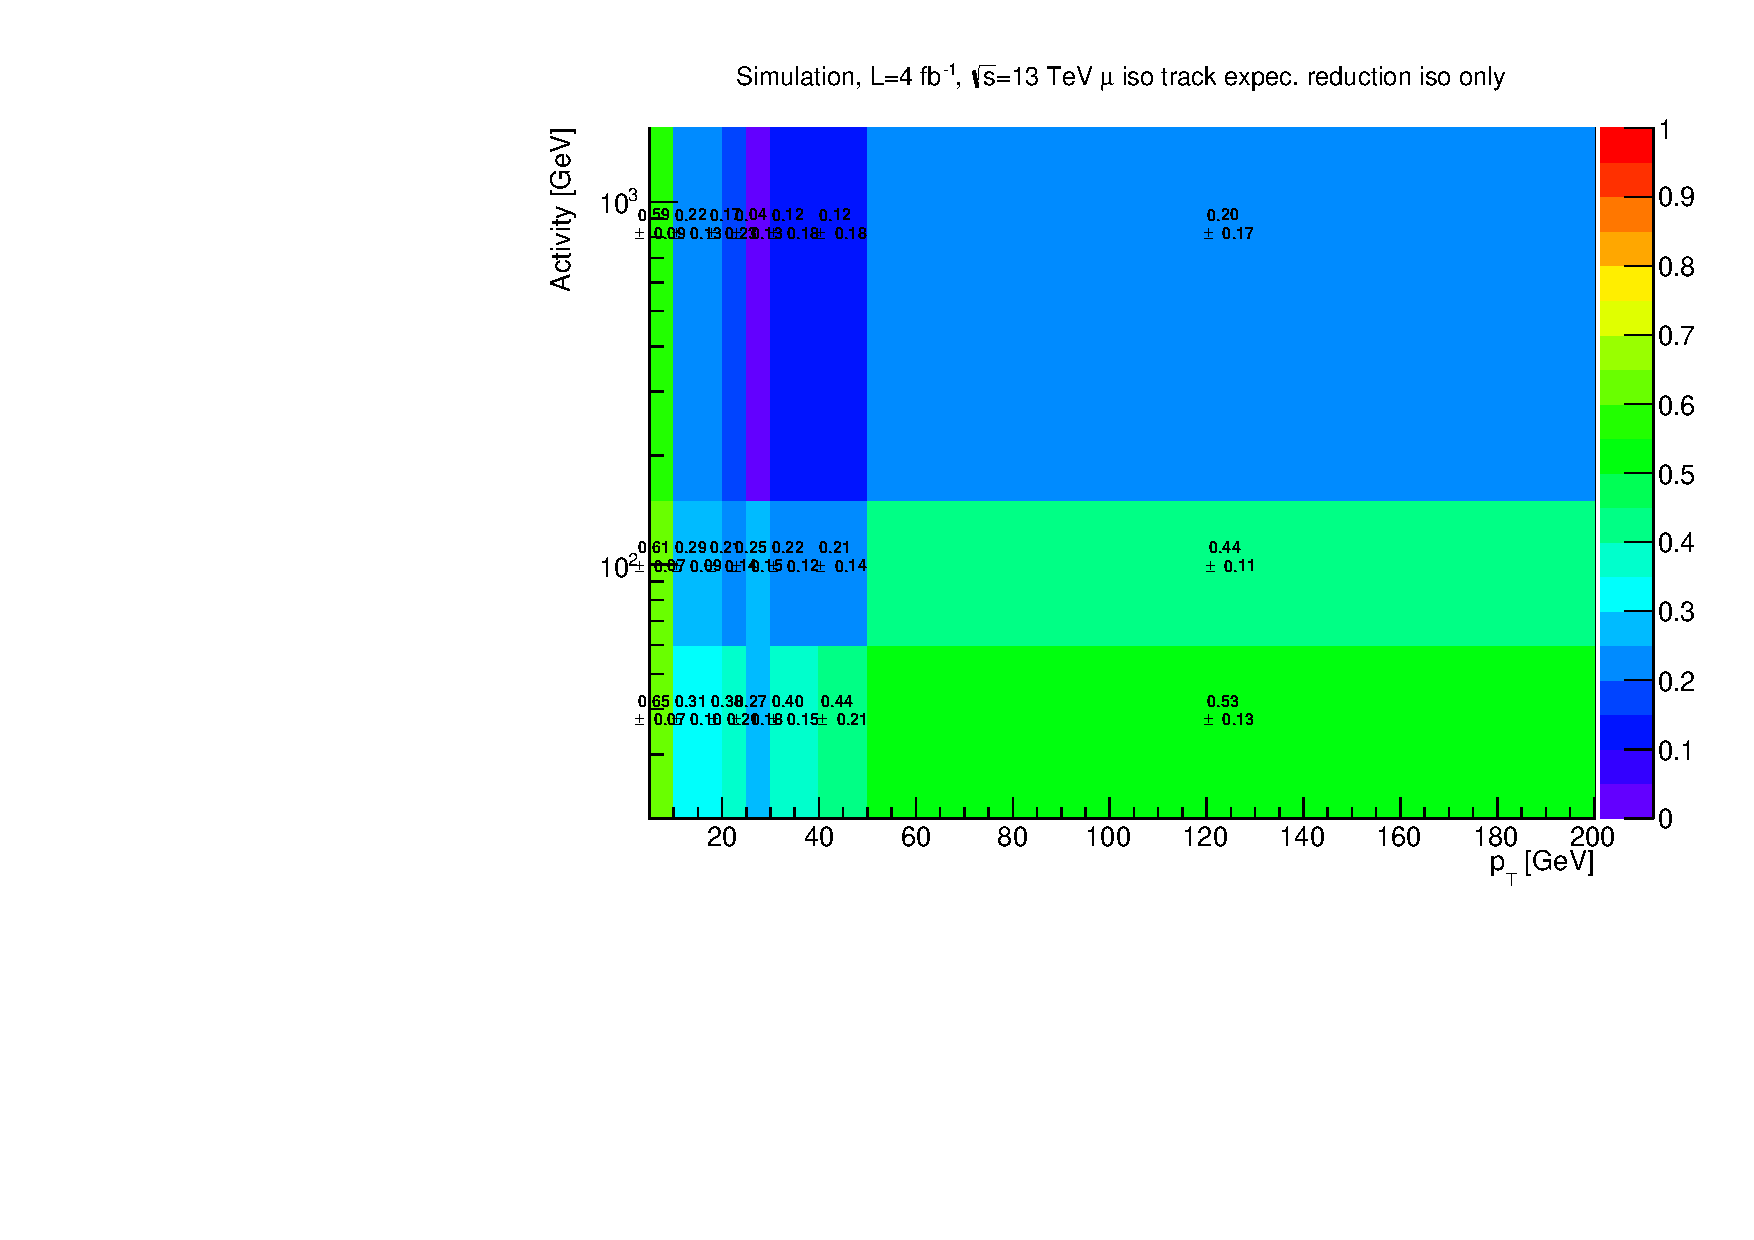
\includegraphics[width=1.\textwidth]{figures/efficiencies/ttbar-wpj/MuIsoTrackGenMuReductionPTActivity.pdf}};
    \begin{scope}[x={(image.south east)},y={(image.north west)}]
%         \draw[red,ultra thick,rounded corners] (0.62,0.65) rectangle (0.78,0.75);
%         \draw[red,ultra thick,rounded corners] (0.60,0.01) rectangle (0.75,0.99); % cordinates unten links(x,y) oben rechts(x,y)
    \end{scope}
   \end{tikzpicture}
   \end{column}
   \begin{column}{0.33\textwidth}
   \begin{itemize}
    \item $\mu$ track DY eff. \\(Tag\&Probe)
   \end{itemize}

    \begin{tikzpicture}
    \node[anchor=south west,inner sep=0] (image) at (0,0) {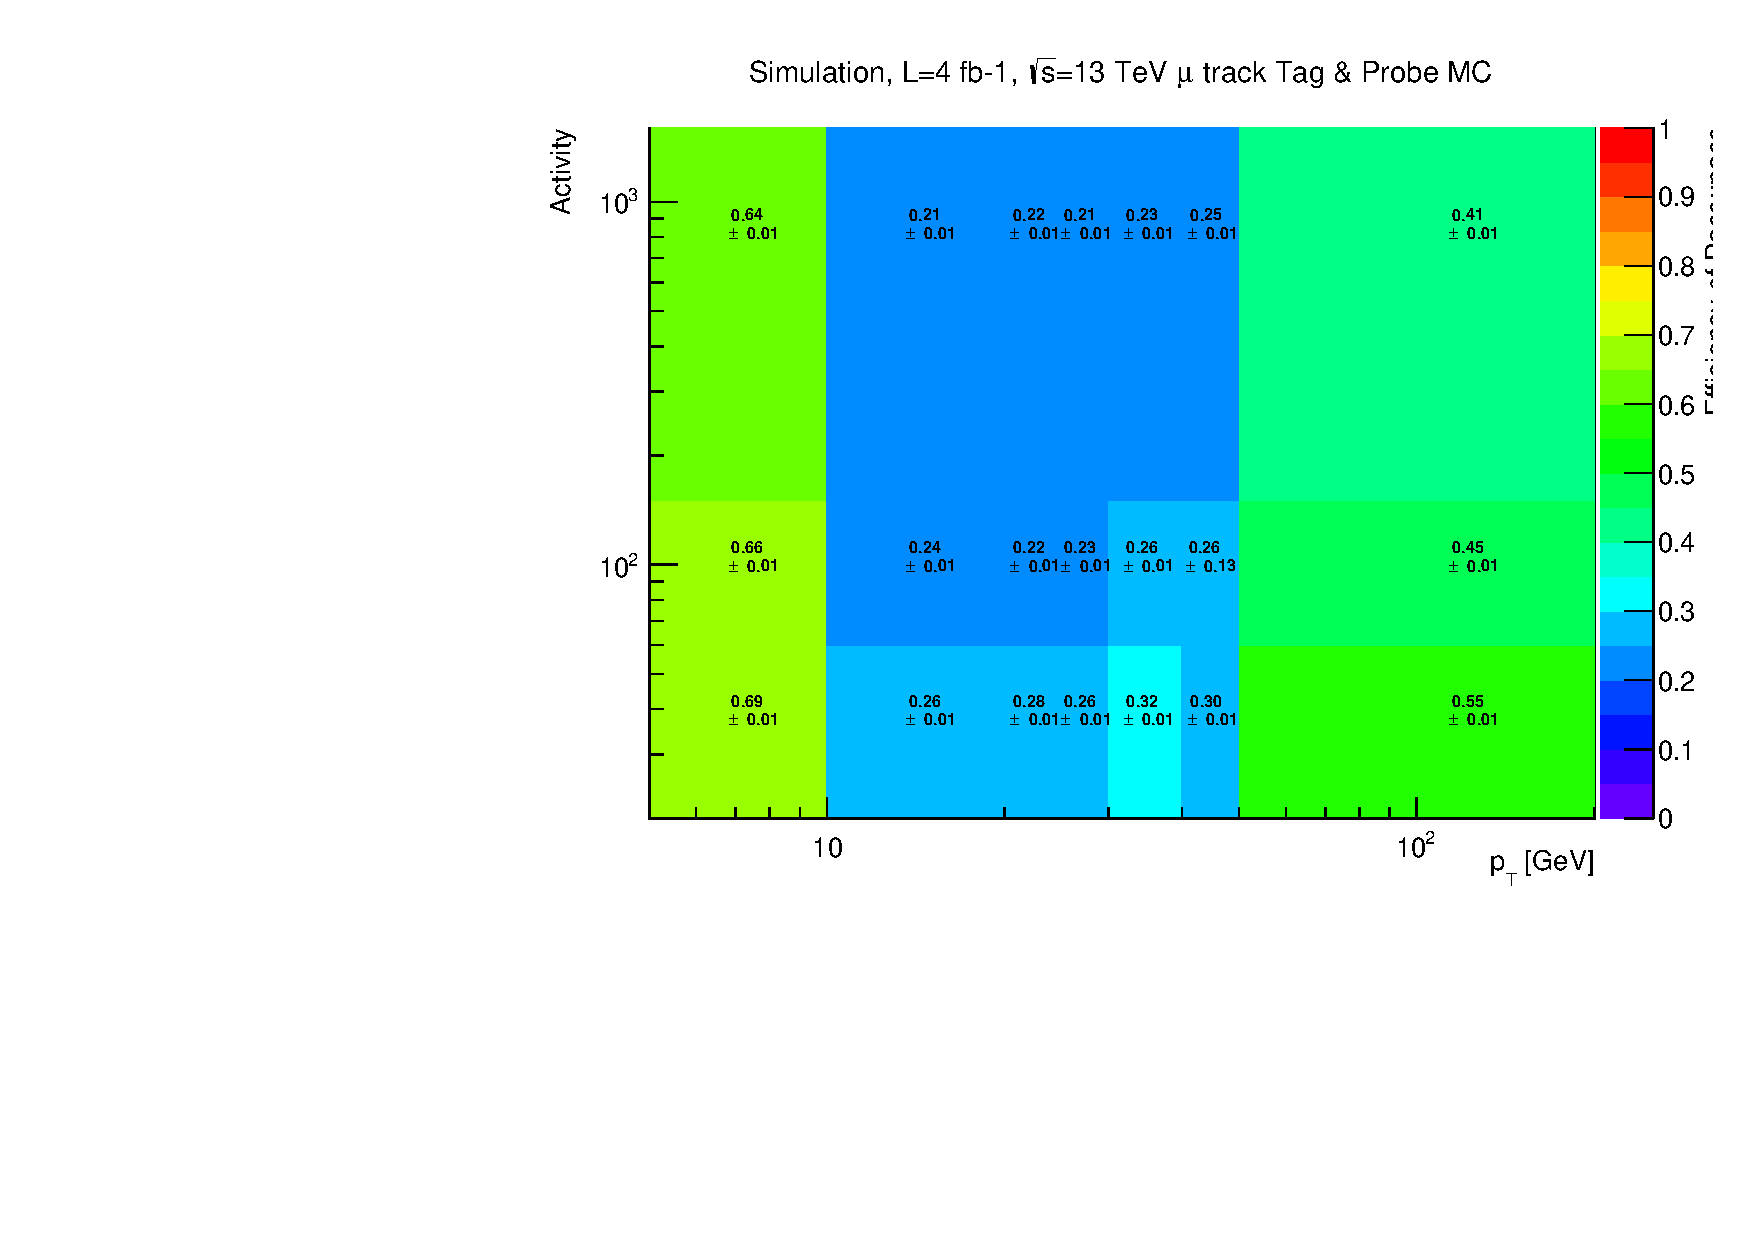
\includegraphics[width=1.\textwidth]{figures/efficiencies/tagandprobe/MuTrackTagAndProbeMC.pdf}};
    \begin{scope}[x={(image.south east)},y={(image.north west)}]
%         \draw[red,ultra thick,rounded corners] (0.62,0.65) rectangle (0.78,0.75);
%         \draw[red,ultra thick,rounded corners] (0.60,0.01) rectangle (0.75,0.99); % cordinates unten links(x,y) oben rechts(x,y)
    \end{scope}
   \end{tikzpicture}
   \end{column}
           \begin{column}{0.33\textwidth}
   \begin{itemize}
    \item Ratio: \ttbar \& \wpj / Tag\&Probe
   \end{itemize}

    \begin{tikzpicture}
     \node[anchor=south west,inner sep=0] (image) at (0,0) {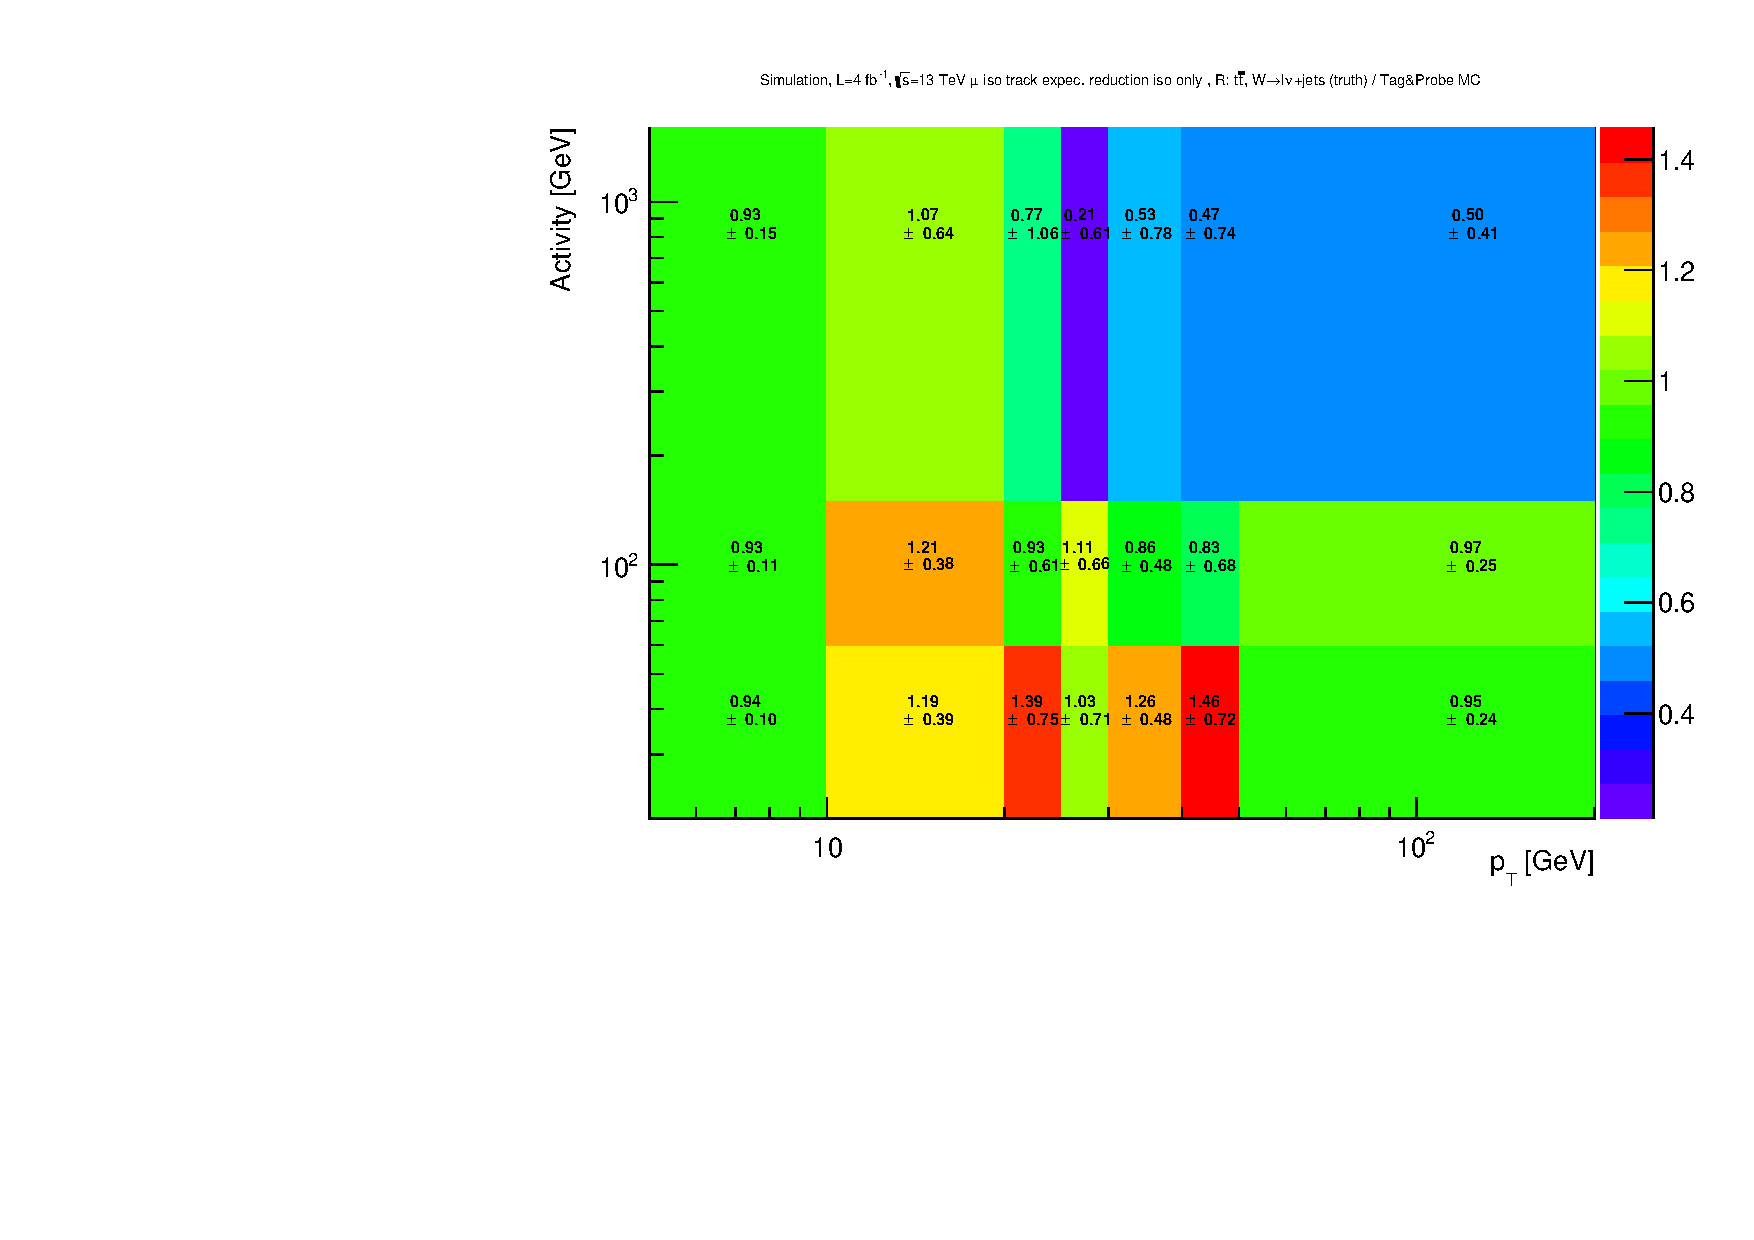
\includegraphics[width=1.\textwidth]{figures/efficiencies/tagandprobe/MuIsoTrackGenMuPTActivity_ratio.pdf}};
    \begin{scope}[x={(image.south east)},y={(image.north west)}]
%         \draw[red,ultra thick,rounded corners] (0.62,0.65) rectangle (0.78,0.75);
%         \draw[red,ultra thick,rounded corners] (0.60,0.01) rectangle (0.75,0.99); % cordinates unten links(x,y) oben rechts(x,y)
    \end{scope}
   \end{tikzpicture}
   \end{column}
  \end{columns}
  \begin{itemize}
   \item Rather good agreement over the full \pt and Activity range
   \item Good agreement in the important $5\leq\pt\leq10\gev$ region
  \end{itemize}


\end{frame}



\begin{frame}
 \frametitle{Comparison \ttbar \& \wpj vs Tag \& Probe Efficiencies}
  \begin{columns}

   \begin{column}{0.33\textwidth}
     \begin{itemize}
   \item e track \ttbar \& \wpj eff. (truth info.)
  \end{itemize}
    \begin{tikzpicture}
    \node[anchor=south west,inner sep=0] (image) at (0,0) {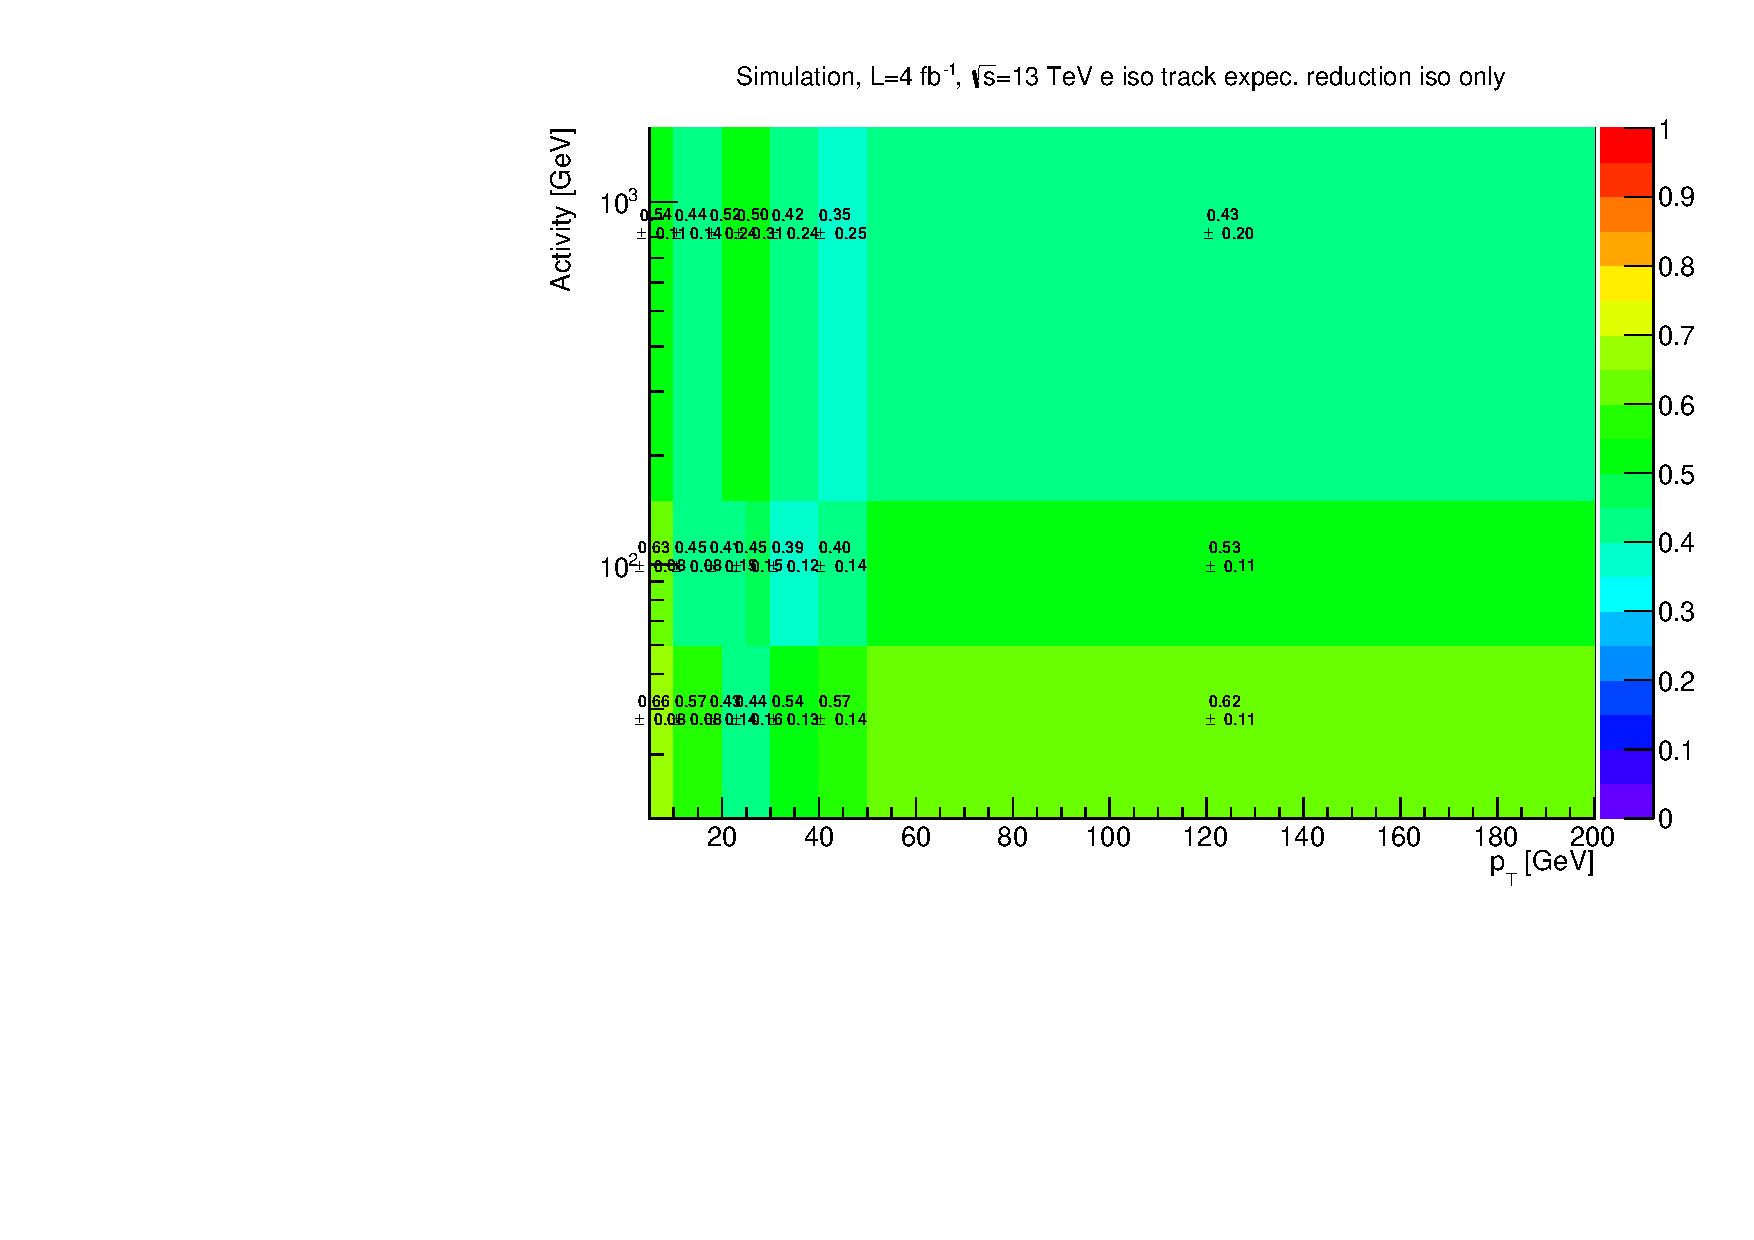
\includegraphics[width=1.\textwidth]{figures/efficiencies/ttbar-wpj/ElecIsoTrackGenElecReductionPTActivity.pdf}};
    \begin{scope}[x={(image.south east)},y={(image.north west)}]
%         \draw[red,ultra thick,rounded corners] (0.62,0.65) rectangle (0.78,0.75);
%         \draw[red,ultra thick,rounded corners] (0.60,0.01) rectangle (0.75,0.99); % cordinates unten links(x,y) oben rechts(x,y)
    \end{scope}
   \end{tikzpicture}
   \end{column}
   \begin{column}{0.33\textwidth}
   \begin{itemize}
    \item e track DY eff. \\(Tag\&Probe)
   \end{itemize}

    \begin{tikzpicture}
    \node[anchor=south west,inner sep=0] (image) at (0,0) {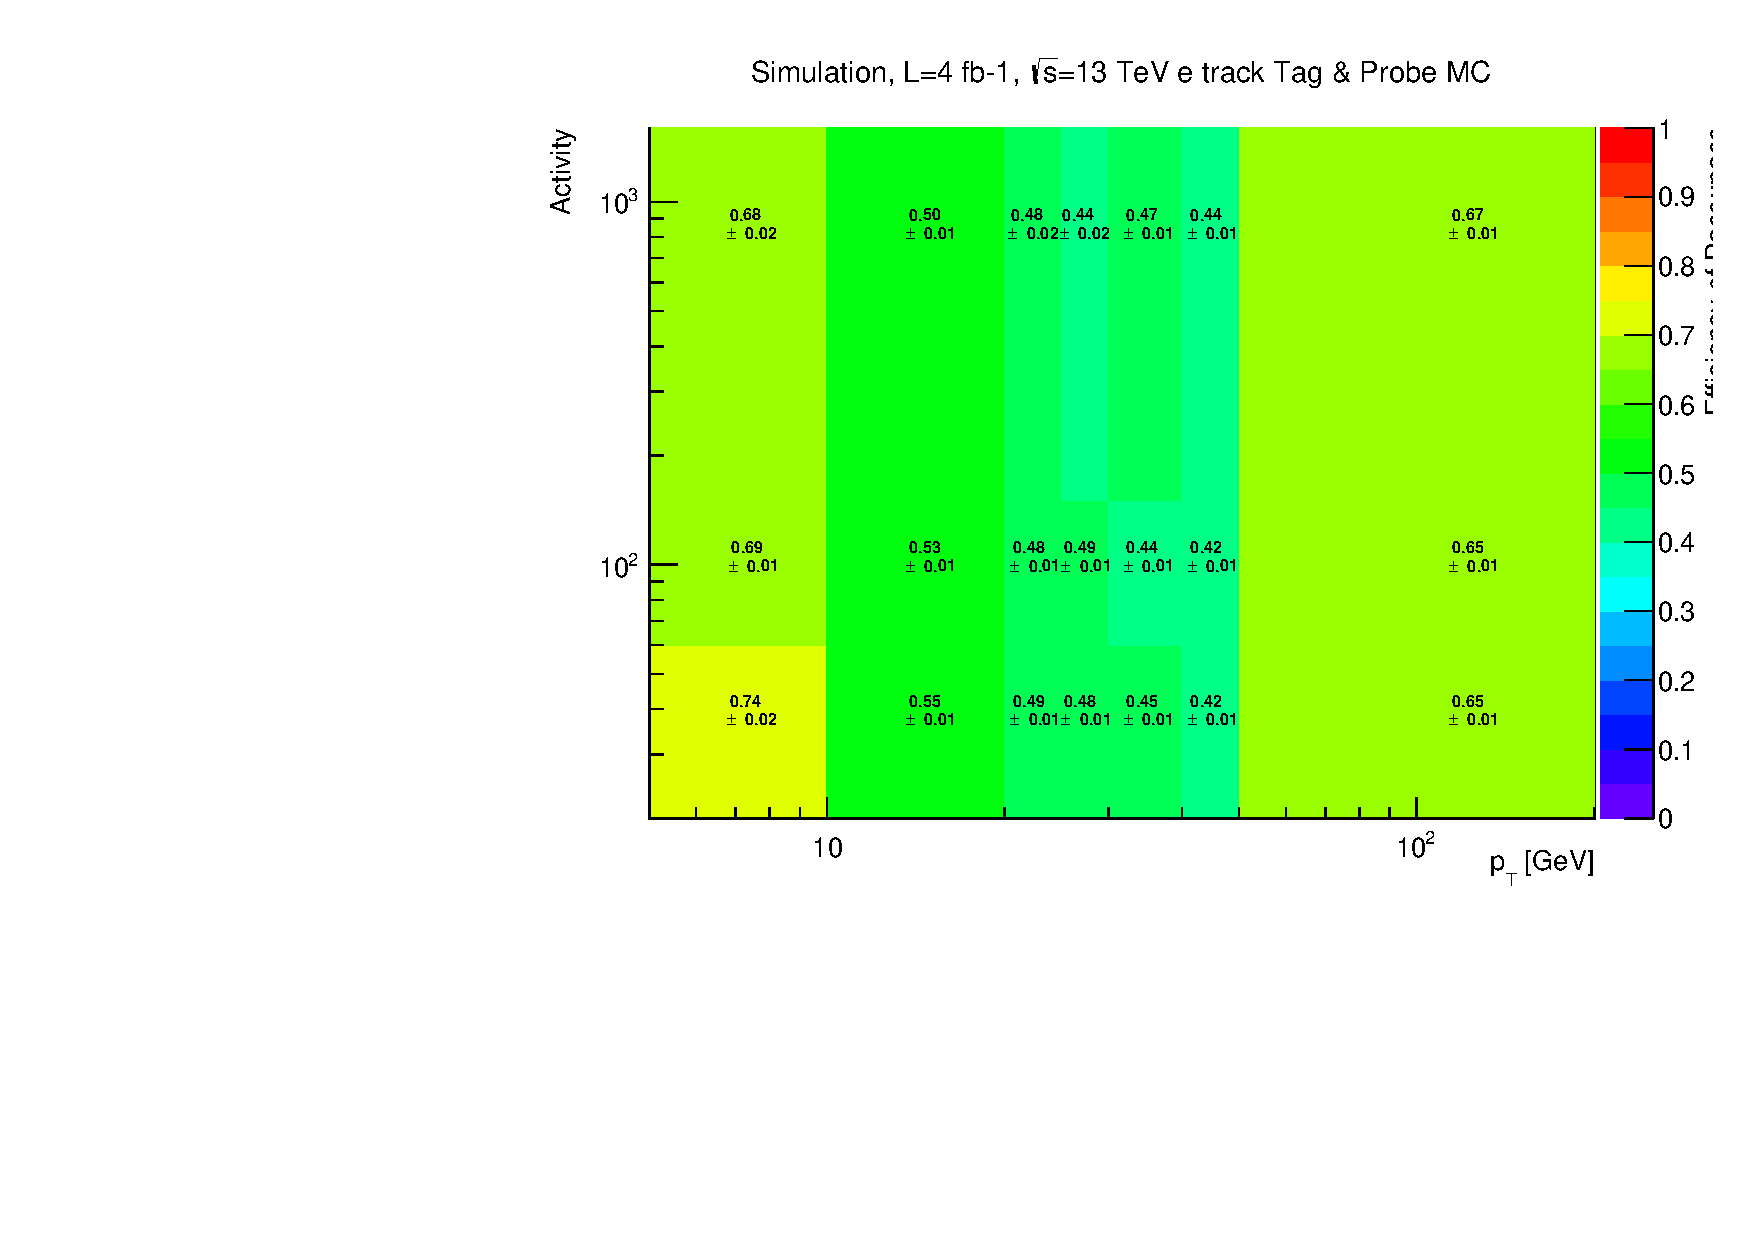
\includegraphics[width=1.\textwidth]{figures/efficiencies/tagandprobe/ElecTrackTagAndProbeMC.pdf}};
    \begin{scope}[x={(image.south east)},y={(image.north west)}]
%         \draw[red,ultra thick,rounded corners] (0.62,0.65) rectangle (0.78,0.75);
%         \draw[red,ultra thick,rounded corners] (0.60,0.01) rectangle (0.75,0.99); % cordinates unten links(x,y) oben rechts(x,y)
    \end{scope}
   \end{tikzpicture}
   \end{column}
           \begin{column}{0.33\textwidth}
   \begin{itemize}
    \item Ratio: \ttbar \& \wpj / Tag\&Probe
   \end{itemize}

    \begin{tikzpicture}
     \node[anchor=south west,inner sep=0] (image) at (0,0) {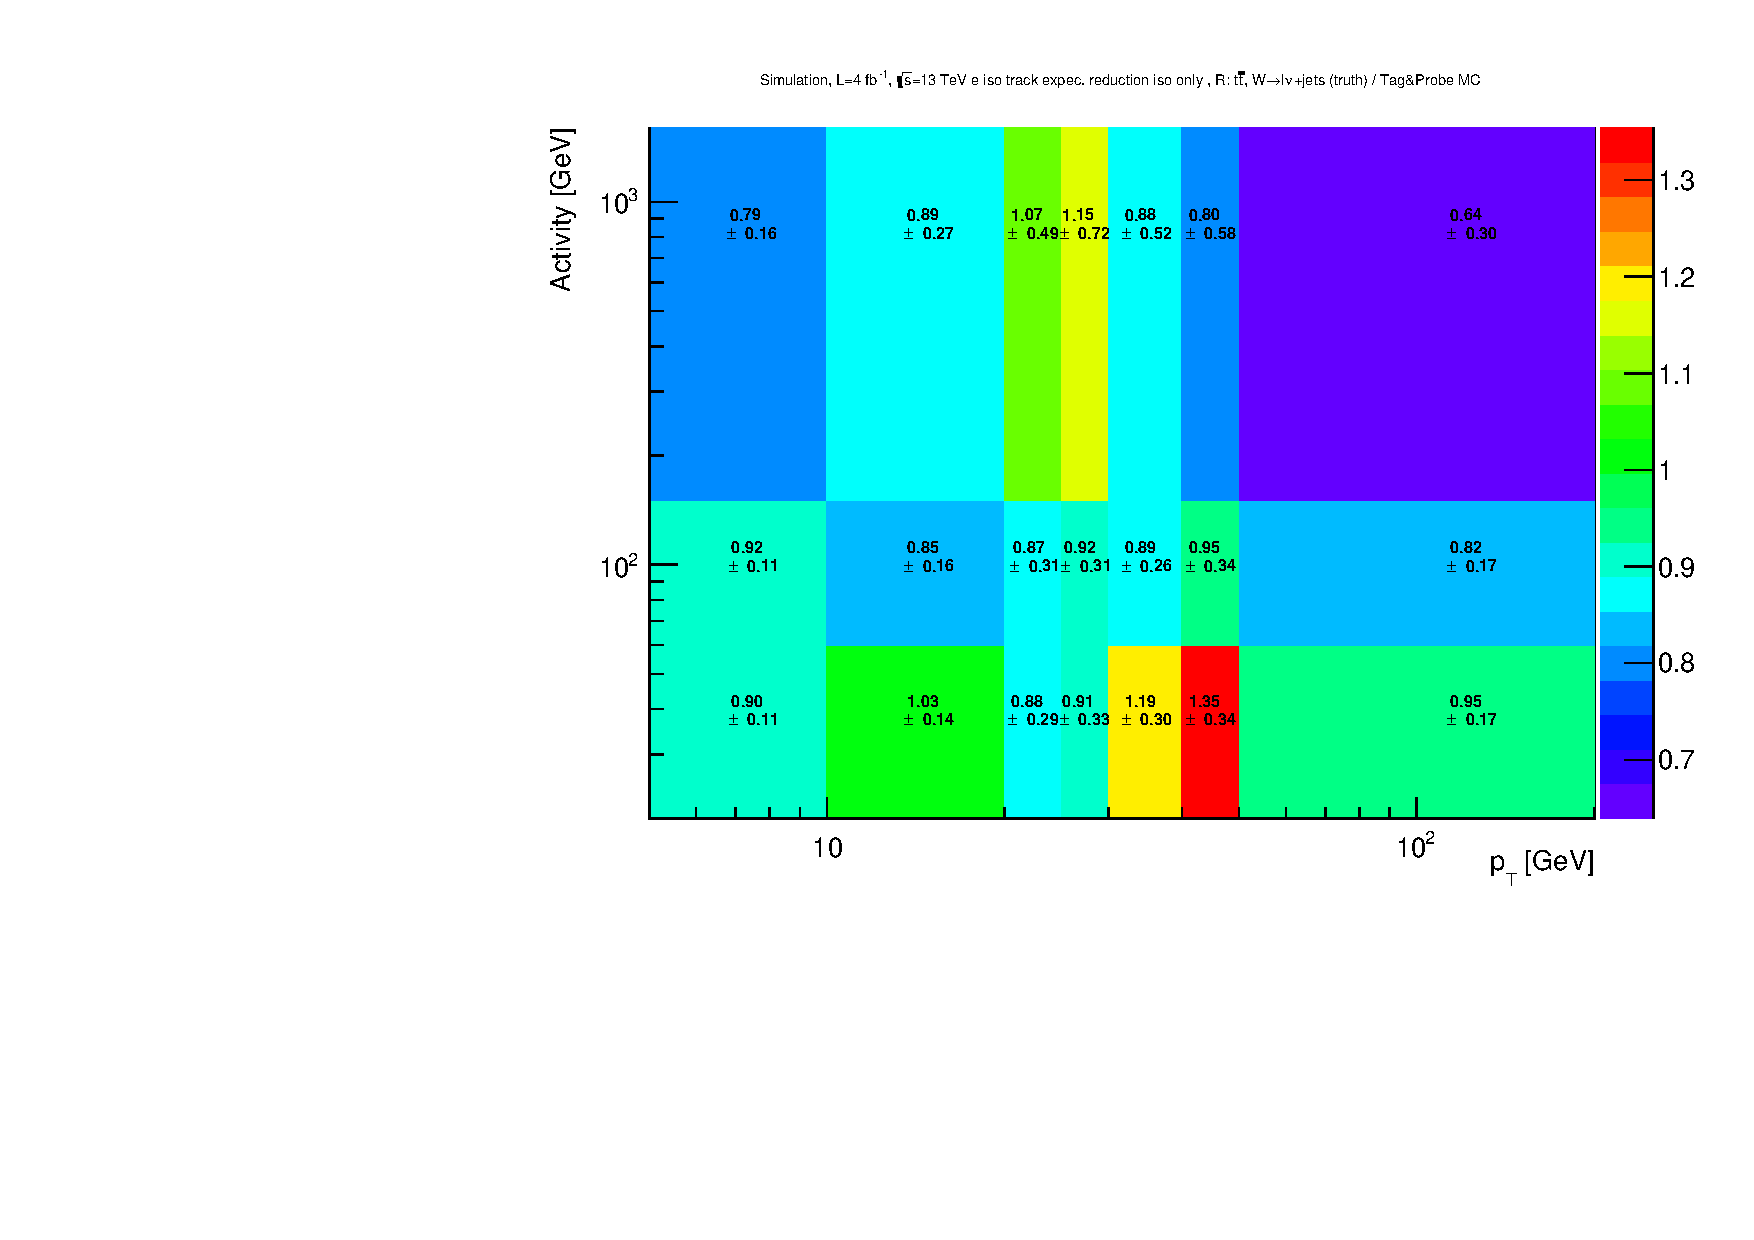
\includegraphics[width=1.\textwidth]{figures/efficiencies/tagandprobe/ElecIsoTrackGenElecPTActivity_ratio.pdf}};
    \begin{scope}[x={(image.south east)},y={(image.north west)}]
%         \draw[red,ultra thick,rounded corners] (0.62,0.65) rectangle (0.78,0.75);
%         \draw[red,ultra thick,rounded corners] (0.60,0.01) rectangle (0.75,0.99); % cordinates unten links(x,y) oben rechts(x,y)
    \end{scope}
   \end{tikzpicture}
   \end{column}
  \end{columns}
  \begin{itemize}
   \item Rather good agreement over the full \pt and Activity range
   \item Reasonable agreement in the important $5\leq\pt\leq10\gev$ region
  \end{itemize}
\end{frame}




% \begin{frame}
%  \frametitle{Iso track reduction by component 1}
%  \begin{overpic}[width=.40\textwidth]{figures/efficiencies/ttbar-wpj/IsoTrackReductionPTActivity.pdf}      %\put(18,36.2){\color{red}\line(1,0){75}}
%       \end{overpic}\\
%  \begin{overpic}[width=.32\textwidth]{figures/efficiencies/ttbar-wpj/MuIsoTrackReductionPTActivity.pdf}      %\put(18,36.2){\color{red}\line(1,0){75}}
%       \end{overpic}
%  \begin{overpic}[width=.32\textwidth]{figures/efficiencies/ttbar-wpj/ElecIsoTrackReductionPTActivity.pdf}      %\put(18,36.2){\color{red}\line(1,0){75}}
%       \end{overpic}
%  \begin{overpic}[width=.32\textwidth]{figures/efficiencies/ttbar-wpj/PionIsoTrackReductionPTActivity.pdf}      %\put(18,36.2){\color{red}\line(1,0){75}}
%       \end{overpic}
% \end{frame}



\begin{frame}
 \begin{block}{}
 \centering
 \Large Backup
 \end{block}
\end{frame}





% --------------------------------------------------

\setcounter{framenumber}{26}

\end{document}

